\documentclass[a4paper,12pt,oneside, bibliography=totoc]
{scrbook}
\usepackage[utf8]{inputenc}
\usepackage{pgf-umlcd}
% Schrift und -kodierung
\usepackage[T1]{fontenc}
\usepackage{lmodern}
\usepackage{tcolorbox}
% Sprache/Silbentrennung
\usepackage[german]{babel} %TODO change to german if desired
\usepackage{booktabs}
\usepackage{amsmath}
\usepackage{floatflt}
\usepackage{float} 
\usepackage{hyperref}
\usepackage{graphicx}
\usepackage{pbox}
\usepackage{algorithmic}
\usepackage{algorithm}
\usepackage{siunitx}
\usepackage[autostyle]{csquotes}
\usepackage{todonotes}
\usepackage{svg}
\usepackage[page, title, titletoc, header]{appendix} %prettier appendix

\svgpath{{../figures/}}

\usepackage[printonlyused]{acronym}
\usepackage{listings} 
\usepackage{subfig}
\lstset{xleftmargin=2em} %Proper indention of listings


\usepackage{tabularx} %For tables
\usepackage{csquotes} %For Quotes





%Footnote Numbering not reset in new chapters
\usepackage{chngcntr}
\counterwithout{footnote}{chapter}


%Remove last point after section/subsections
\renewcommand{\autodot}{}

\usepackage[htt]{hyphenat} %damit texttt noch Linebreaks mit Silbentrennung erzeugt
\newcommand{\code}[1]{\texttt{#1}} %Programmcode im Textfluss in passendem Font ausgeben




%Literatur
%Ordering in references checken, vermutlich was mit style=numeric zu tun
\usepackage[
   backend=biber,
   sorting= none,
   firstinits=true,
   date=long,
   urldate=long
]{biblatex}
\addbibresource{database.bib}
%\addbibresource{literatur2.bib}


\usepackage[]{hyperref}

\begin{document}
\frontmatter %roman page numbers





	\titlehead{
	\begin{center}
	   \includegraphics[width=10cm]{figures/unilogo.pdf}\\
	   	Institute of Computer Science, Software Engineering Group
	\end{center}
	}
	\subject{Bachelorarbeit}
	\title{Entwicklung einer Anwendung zur Bewertung der Dokumentation von Quellcode mithilfe von GitHub Actions
 }
	\author{Timo Schoemaker\\ Immatrikulationsnummer: 978621} %engl. Matriculation Number

	\date{\today\\
	Erstbetreuer: Prof. Dr.-Ing. Elke Pulvermüller \\ %Deutsch: Erstebetreuer
	Zweitbetreuer: Nils Baumgartner, M. Sc.} %Deutsch: Zweitbetreuer
	
	\maketitle
	
	\clearpage
	
	\addchap*{Abstract}
\textbf{Deutsch}
Die Softwaredokumentation ist ein essenzieller Bestandteil der heutigen Softwareentwicklung geworden. Nichtsdestotrotz leidet die Qualität der Dokumentation häufig und viele Entwickler sind nicht motiviert genug, um eine gute Dokumentation zu schreiben. Das Ziel dieser Arbeit ist es, ein Tool zu entwickeln, dass exemplarisch die Dokumentationsqualität in Java-Programmen analysiert und mittels verschiedener Metriken (Anteil dokumentierter Komponenten an allen Komponenten, Flesch-Score, Kohärenz und Nichterwähnung von Randfällen) bewertet. Dieses Tool ist in GitHub Actions eingebunden, um den Entwickler bei einer sehr schlechten Dokumentationsqualität zu warnen und gegebenenfalls Mergevorgänge zu verhindern.

%\linebreak
\bigskip

\noindent
%\bigskip
\textbf{English} 
The software documentation has become an integral part of software development. Nevertheless, the quality of the documentation is often poor and developers are often not motivated to write good documentation. The goal of this thesis is to develop a tool that can analyze the documentation quality of Java applications by applying different metrics (percentage of documented components in all components, Flesch score, coherence, not mentioning the handling of edge cases). This tool will be integrated in GitHub Actions to warn the developer about poor software documentation quality and to prevent a merge if the quality becomes too poor.  

%TODO Bis jetzt nur Osi Abstract, evtl. etwas ausführlicher für Masterarbeit


	\clearpage
	
	\tableofcontents
	\clearpage

	




\lstdefinelanguage{YAML}{
  morekeywords=
  {
    name:,on:,jobs:,steps:,uses:,run:,echo,workflow_dispatch:,description:,inputs:,required:,default:,runs-on:,using:,main:,with:,author:, absolute_threshold:
  },
  keywordstyle=\color{black}\bfseries,
  ndkeywords={false,compf/JavaDocEvaluator@action},
  ndkeywordstyle=\color{black}\bfseries,
  identifierstyle=\color{black},
  sensitive=false,
  comment=[l]{//},
  morecomment=[s]{/*}{*/},
  commentstyle=\color{purple}\ttfamily,
  %stringstyle=\color{red}\ttfamily,
  morestring=[b]',
  morestring=[b]",
  alsodigit={:},
  alsoletter={/,@,-}
}




\lstdefinelanguage{ANTLR}{
  keywords=
  {
   formalParameter:,variableModifier:,typeType:,variableDeclaratorId:,JCOMMENT:
  },
  keywordstyle=\color{black}\itshape,
  identifierstyle=\color{black},
  sensitive=false,
  comment=[l]{//},
  morecomment=[s]{/*}{*/},
  commentstyle=\color{purple}\ttfamily,
  morestring=[b]',
  morestring=[b]",
  alsodigit={:},
}

\lstdefinelanguage{JSON}{
    tabsize             = 4,
    showstringspaces    = false,
    keywords            = {false,true,include,exclude,metrics,metric_name,weight,unique_name,params,absolute_threshold,builder,relative_threshold},
    alsoletter          = 0123456789.*,
    ndkeywordstyle         = \color{red},
  keywordstyle=\color{black}\bfseries,
}





\lstdefinelanguage{javascript}{
  keywords={typeof, new, true, false, catch, function, return, null, catch, switch, var, if, in, while, do, else, case, break,let,this,private},
  keywordstyle=\color{black}\bfseries,
  identifierstyle=\color{black},
  sensitive=true,
  comment=[l]{//},
  morecomment=[s]{/*}{*/},
  commentstyle=\color{purple}\ttfamily,
  stringstyle=\color{red}\ttfamily,
  morestring=[b]',
  morestring=[b]",
}
%\ac{Abk.}         % fügt die Abkürzung ein, außer beim ersten Aufruf, hier wird die Erklärung mit angefügt
%\acs{Abk.}        % fügt die Abkürzung ein
%\acf{Abk.}        % fügt die Abkürzung UND die Erklärung ein
%\acl{Abk.}        % fügt nur die Erklärung ein

%\chapter*{Acronyms}
\addchap{Acronyms}

%%%%%%%%%%%%%%%%%%%%%%%
\begin{acronym}[E/E/PE] %sorgt fuer proper indention
	\acro{ATL}{\emph{Atlas Transformation Language}}
	\acro{BMWi}{\emph{Bundesministerium für Wirtschaft und Energie}}
	\acro{CIM}{\emph{Computation-Independent Model}}
	\acro{CDC}{\emph{Code-level design choice}}
	\acro{CR}{\emph{Code-level requirement}}
	\acro{CI/CD}{Continuous Integration/Continuous Delivery}
	\acro{CRC}{\emph{Cycling Redundancy Checks}}
	\acro{E/E/PE}{\emph{Electrical/Electronic/Programmable Electronic}}
	\acro{ECC}{\emph{Error Detecting and Correcting Codes}} 
	\acro{EMF}{\emph{Eclipse Modeling Framework}}
	\acro{EGL}{\emph{Epsilon Generation Language}}
	\acro{EOL}{\emph{Epsilon Object Language}}
	\acro{Epsilon}{\emph{Extensible Platform of Integrated Languages for mOdel maNagement}}
	\acro{FS}{\emph{Functional Safety}}
	\acro{HAL}{\emph{Hardware Abstraction Layer}}
	\acro{HolMES}{\emph{Holistische Modell-getriebene Entwicklung für Eingebettete Systeme unter Berücksichtigung unterschiedlicher Hardware-Architekturen}}
	\acro{IDE}{\emph{Integrated Development Environment}}
	\acro{JVM}{\emph{Java Virtual Machine}}
	\acro{LOC}{\emph{Lines of Code}}
	\acro{MISRA}{\emph{Motor Industry Software Reliability Association}}
	\acro{MBU}{\emph{Multi Bit Upset}}
	\acro{MDA}{\emph{Model Driven Architecture}}
	\acro{MDC}{\emph{Model-level design choice}}
	\acro{MDD}{\emph{Model Driven Development}}
	\acro{MDE}{\emph{Model Driven Engineering}}
	\acro{MOF}{\emph{Meta Object Facility}}
	\acro{MR}{\emph{Model-level requirement}}
	\acro{NLP}{\emph{Natural Language Processing}}
	\acro{OCL}{\emph{Object Constraint Language}}
	\acro{OMG}{\emph{Object Management Group}}
	\acro{PIM}{\emph{Platform-Independent Model}}
	\acro{PSM}{\emph{Platform-Specific Model}}
	\acro{SER}{\emph{Soft Error Rate}}
	\acro{SEU}{\emph{Single Event Upset}}
	\acro{TMR}{\emph{Triple Modular Redundancy}}
	\acro{UML}{\emph{Unified Modeling Language}}
	


%\acro{cMOF}{\emph{complete MOF}}
%\acro{eMOF}{\emph{essential MOF}}

%	\acro{ETL}{\emph{Epsilon Transformation Language}}
%	\acro{EWL}{\emph{Epsilon Wizard Language}}

	
\end{acronym} %See inside for usage of acronmys
\mainmatter %switch roman auf arabic page numbers



\chapter{Einführung}
\setcounter{page}{1} %Seitenzahlen hier mit 1 anfangen

	%Include text from other files into the document --> great for structuring
	\label{sec:introduction}

Ein wichtiger Bestandteil der Softwareentwicklung von heute ist die Softwaredokumentation. Dies liegt unter anderem daran, dass die Größe von Softwareprojekten steigt, sodass kein Entwickler das gesamte Programm im Überblick hat und daher zusätzliche Informationen neben dem Code benötigt \cite[S. 1]{StaticAnalysis:AnIntroduction:TheFundamentalChallengeofSoftwareEngineeringisOneofComplexity.}. Nichtsdestotrotz wird die Softwaredokumentation von Entwicklern oft vernachlässigt \cite[S. 83]{Qualityanalysisofsourcecodecomments}.  Die Gründe für schlechte Dokumentation sind vielfältig. Das Schreiben der Dokumentation wird oft als mühevoll empfunden und erfordert Fähigkeiten, die ein Programmierer nichts zwangsläufig hat\cite[S. 70]{AutomaticQualityAssessmentofSourceCodeComments:TheJavadocMiner} \cite[S. 593]{Softwareengineeringandsoftwaredocumentation:aunifiedlongcourse}.  

Die mangelhafte Dokumentation führt dazu, dass nicht nur nachfolgende Entwickler Probleme mit dem Codeverständnis haben, sondern auch der Entwickler eines Moduls nach einer längeren Pause Zeit aufbringen muss, um den Code wieder zu verstehen. \cite[S. 511]{vestdam} Auch für Kunden/Auftraggeber ist eine gute Dokumentation wichtig, da gut dokumentierte Software tendenziell besser wartbar ist und somit mehr Nutzen bringt \cite[S. 83]{Qualityanalysisofsourcecodecomments}\cite[S. 1]{SoftwareDocumentationManagementIssuesandPractices:ASurvey}.


Dass in vielen Fällen die Softwaredokumentation vernachlässigt wird, ist durch viele Studien belegt. Eine Umfrage aus dem Jahr 2002 mit 48 Teilnehmern belegt beispielsweise, dass Anforderungs- oder Spezifikationsdokumente nur selten bei Änderungen am Quellcode angepasst werden. Außerdem finden 54\% der befragten Entwickler  Textverarbeitungsprogramme wie Word für hilfreich, die nicht für Dokumentationszwecke entwickelt wurden.Diese Programme sind leicht zu bedienen und sehr flexibel, aber nicht effizient  \cite[S. 28-29]{TheRelevanceofSoftwareDocumentationToolsandTechnologies:ASurvey}. 

Eine weitere Studie aus dem Jahr 2019 verdeutlicht viele Aspekte aus der vorgenannten Umfrage. Es wurden dabei Daten aus Stack Overflow, GitHub Issues und Pull Requests und Mailing-Listen automatisiert heruntergeladen und dann von den Autoren analysiert, ob und inwieweit mit mangelhafter Softwaredokumentation zu tun haben.  Die Studie liefert klare Indizien dafür, dass die Softwaredokumentation in vielen Fällen nicht komplett, nicht auf dem neuesten Stand oder sogar nicht korrekt ist. Des Weiteren ist die Softwaredokumentation nicht gut nutzbar oder schlecht lesbar, sodass der Vorteil verloren geht\cite[S.1201 -1204]{SoftwareDocumentationIssuesUnveiled}.







\section{Zielsetzung}
Aus diesen Gründen ist eine regelmäßige Rückmeldung über die Dokumentation von hoher Bedeutung. Eine Möglichkeit, dieses Feedback zu geben, sind spezielle Metriken, welche eine numerische Auskunft über die Qualität der Softwaredokumentation liefern. Diese Metriken liefern dem Programmierer eine gute Einschätzung, ob die Softwaredokumentation ausreichend ist oder eine Verbesserung sinnvoll wäre. Da es im Bereich der Softwaredokumentation, verschiedene Metriken gibt, ist es sinnvoll mehrere Metriken zu verwenden. Die Ergebnisse aller Metriken können dann kombiniert werden. Dabei ist es auch ratsam, die Metriken zu gewichten, weil nicht jede Metrik die gleiche Zuverlässigkeit und Relevanz besitzt.

Damit das Feedback über die Softwaredokumentation auch wahrgenommen wird, sollte die Qualität regelmäßig  überprüft werden. Dies kann automatisiert in \ac{CI/CD}-Prozess erfolgen, bei dem Software kontinuierlich getestet und für den Release (z.~dt. Veröffentlichung) vorbereitet werden kann. Durch CI/CD können Unternehmen effizienter und besser Software entwickeln. So konnte die ING NL die gelieferten Function-Points vervierfachen und die Kosten für einen Function-Point auf einen Drittel reduzieren \cite[S. 520]{Vassallo2016}.

Basierend auf diesen Überlegungen soll ein Tool(z.dt. Werkzeug) entwickelt werden. Dieses Tool soll ein gegebenes Software-Projekt analysieren und eine numerische Bewertung darüber abgeben, die eine heuristische Aussage über die Qualität der Softwaredokumentation trifft.  Dabei soll das Tool primär für Javadoc konzipiert werden, allerdings soll während der Entwicklung auch darauf geachtet werden, dass eine Portierung auf eine andere Programmiersprache möglichst einfach wird und die Bewertung der Dokumentation unabhängig von der Programmiersprache funktioniert. Ziel dabei soll es nicht sein, dass jede Komponente (wie z.~B. Methoden oder Klassen) dokumentiert sein muss, sondern dass die wichtigen Komponenten eine gute Dokumentationsqualität haben und somit die Wartung vereinfacht wird. 



\section{Gliederung}
Zur Umsetzung der Bachelorarbeit wird zunächst ein Einblick in das Thema Code-Smell (Kapitel \ref{chapter:code_smell}) gegeben, da schlechte Softwaredokumentation als Code-Smell angesehen werden kann. Anschließend muss der Begriff der Softwaredokumentation genauer definiert werden, da der Begriff so noch sehr unklar ist    (Kapitel \ref{chapter:documentation}). Zudem wird eine Einführung in Javadoc gegeben, da dieses Tool am Ende der Bachelorarbeit hauptsächlich Java und Javadoc verarbeiten soll (Kapitel \ref{chapter:javadoc}). 
Außerdem werden einige verwandte Programme vorgestellt, die ebenfalls die Qualität der Softwaredokumentation analysieren können. Des Weiteren werden einige wissenschaftliche Arbeiten zusammengefasst, die sich ebenfalls mit der Analyse von Softwaredokumentationen beschäftigen.

Um das Programm in dem \ac{CI/CD}-Prozess einzubinden, wird \enquote{GitHub Actions} verwendet. Dieser Service der Plattform GitHub \footnote{\href{https://github.com/}{Github Website (besucht am 07.01.2022)}} ermöglicht es, eigene Programme (oder Programme aus einer großen Auswahl von anderen Programmierern) auf den Quelltext auszuführen.  Diese Programme können dann Fehlermeldungen werfen, wenn es irgendwelche Probleme mit dem Quelltext gibt, sodass der Entwickler darauf aufmerksam wird und die Probleme lösen kann. Mit dieser Plattform ist damit möglich, die Qualität der Softwaredokumentation regelmäßig zu prüfen und bei einer deutlichen Unterschreitung den Entwickler durch Fehlermeldungen zu warnen.  Eine kurze Einführung in GitHub Actions erfolgt in Kapitel \ref{chapter:github_actions}

Danach wird erläutert, wie das Programm entwickelt wurde und welche Herausforderungen zu bewältigen waren. Zunächst muss das Tool die Dateien finden, die vermutlich Softwaredokumentation enthalten und als relevant angesehen werden. Jede dieser Datei muss dann in einzelne Komponenten zerlegt werden, wobei jede Komponente einen Verweis auf ihre Dokumentation (z~B. Javadoc) enthält. Als Komponente im Sinne dieser Bachelorarbeit werden dabei Klassen, Schnittstellen, Methoden und Felder verstanden.

Als nächstes wird beschrieben, wie das Tool zu einer numerischen Bewertung der Qualität der Softwaredokumentation gelangt. Dazu werden verschiedene Metriken angewendet, die in Kapitel \ref{chapter:metrics} erläutert werden. Das Ergebnis jeder Metrik wird dann geeignet aggregiert, damit der Benutzer des Tools eine grobe Einschätzung der Qualität der Dokumentation hat. Beispielsweise kann ein arithmetischer Mittelwert oder ein gewichteter Mittelwert gebildet werden. 

In Anschluss wird in Kapitel \ref{chapter:github_actions_impl}  wird die Einbindung des Tools in GitHub Actions erläutert. Dazu muss das Programm in ein kompakteres Format gebracht werden und in einer separaten Branch in GitHub hochgeladen werden. 

Anschließend soll das Tool mit anderen Tools, die ebenfalls die Dokumentationsqualität bewerten können, verglichen werden. Dazu werden ausgewählte Java-Projekte aus GitHub mit allen Tools analysiert und die Ergebnisse der Tools verglichen. 








\begingroup
\renewcommand{\cleardoublepage}{} % TODO maybe removing this and next
\renewcommand{\clearpage}{}
\chapter{Grundlagen}
\endgroup

	%Multiple input files for larger chapters are also possible
	\label{sec:background}
In diesem Kapitel werden die wichtigen Grundlagen erläutert, die nötig sind, um das Problem mangelhafter Softwaredokumentation zu lösen.  Dazu  wird der Begriff \enquote{Softwaredokumentation} genauer definiert. Außerdem wird eine Einführung in Code-Smells gegeben.  Anschließend gibt es eine Einführung in Javadoc gegeben, dessen Analyse der Schwerpunkt dieser Bachelorarbeit ist. Danach wird die \ac{CI/CD}-Plattform \enquote{GitHub Actions} präsentiert, die genutzt werden soll, um die Dokumentationsqualität regelmäßig zu messen. Am Ende werden weitere Tools vorgestellt, die fehlerhafte Dokumentationen erkennen. Außerdem werden wissenschaftliche Arbeiten zusammengefasst, die sich ebenfalls mit der Thematik \enquote{Softwaredokumentation} befassen. 
 

\section{Softwaredokumentation}\label{chapter:documentation}
Um den Begriff \enquote{Softwaredokumentation} zu definieren, sollte zunächst der Begriff \enquote{Dokumentation} definiert werden. Das IEEE  definiert diesen Begriff als jede textliche oder bildliche Information, welche Aktivitäten, Anforderungen, Abläufe oder Ergebnisse beschreibt, definiert, spezifiziert, berichtet oder zertifiziert \cite[S. 28]{IEEEStandardGlossaryofSoftwareEngineeringTerminology}. Somit beschreibt eine Dokumentation, wie sich eine Komponente aufgebaut ist oder wie sie sich verhält.

Diese abstrakte Definition lässt sich so auf Softwareentwicklung übertragen. In \cite[S. 125]{Softwaredocumentationandstandards} wird Softwaredokumentation als eine Sammlung von technischen Informationen dargestellt, die für Menschen lesbar sind und welche die Funktionen, Benutzung oder das Design eines Softwaresystems beschreiben. So beschreibt Donald E. Knuth in \cite[S. 97]{LiterateProgramming}, dass die Hauptaufgabe beim Programmieren nicht sein sollte, einen Computer zu erklären, was er machen sollte, sondern anderen Menschen zu erklären, was der Computer machen sollte. Beispiele für Softwaredokumentation sind Kommentare,  UML-Diagramme, Readme-Dateien oder Handbücher.

Im Kontext dieser Bachelorarbeit sollen allerdings nur bestimmte Arten der Softwaredokumentation betrachtet werden, da eine umfassende Betrachtung innerhalb der vorgegebenen Zeit nicht möglich ist.  Zwar wären Readme-Dateien oder UML-Diagramme für eine Bewertung auch interessant, allerdings sind diese nicht so stark mit dem dazugehörigen Code verknüpft, sondern befinden sich in externen Dateien, sodass eine Verarbeitung ungleich schwieriger wäre.

Aus diesen Grund konzentriert sich diese Bachelorarbeit nur auf Kommentare. Studien zeigen, dass Kommentare eine hohe Relevanz in der Softwareentwicklung haben, sodass eine Analyse der Kommentare eine gute Annäherung an die tatsächliche Qualität der Dokumentation geben kann \cite[S. 71]{AStudyoftheDocumentationEssentialtoSoftwareMaintenance}. Dabei sollen nicht alle Kommentare betrachtet werden, sondern nur eine bestimmte Kategorie von Kommentaren, die besonders leicht verarbeitbar sind, sodass aus ihnen viele Informationen extrahiert werden können und die Bewertung dadurch genauer werden kann. 

Für diese Bachelorarbeit werden daher nur bestimmte Inline-Kommentare im Quellcode betrachtet, die ein Spezialfall von normalen mehrzeiligen Kommentaren sind.
Diese Kommentare werden wie normale Kommentare erkannt und werden daher nicht Bestandteil des kompilierten Programms. Nichtsdestotrotz haben diese spezifischen Kommentare aber eine bestimmte Struktur, die eine leichte Verarbeitung durch Computerprogramme ermöglicht und gleichzeitig trotzdem für Menschen lesbar bleibt. In vielen Fällen werden diese Kommentare einer bestimmten Komponente zugeordnet, wobei dies dadurch geschieht, dass der Kommentar direkt vor dieser Komponente steht. Ein Beispiel dafür ist Javadoc, da jeder Javadoc-Kommentar auch ein gültiger mehrzeiliger Kommentar ist.





\section{Code Smell}\label{chapter:code_smell}
Der Begriff Code-Smell (z.~dt. übelriechender Code)  wurde von Kent Beck in \cite[S. 71 ff.]{fowler2019refactoring}  vorgeschlagen, um Quellcode zu beschreiben, bei dem Refactoring (z.~dt. Restrukturierung) sinnvoll ist. Bestimmte Strukturen im Quellcode deuten darauf hin, dass der Code verbessert werden sollte, da ansonsten die zukünftige Wartbarkeit des Codes verringert wird. Beispiele sind schlecht gewählte Namen für Variablen oder Methoden, duplizierter Code, lange Methoden oder globale Daten. In bestimmten Situationen werden Kommentare ebenfalls als Code-Smell klassifiziert, da sie auf komplizierten  Code hindeuten können oder der Name einer Komponente schlecht gewählt wurde. Daher sollte geprüft werden, ob nach einem Refactoring die Kommentare noch notwendig sind.

Nach \cite[S. 249-250]{JavadocViolationsandTheirEvolutioninOpen-SourceSoftware} kann eine mangelhafte Dokumentation als Code-Smell bezeichnet werden, da sie die Wartbarkeit der Software beeinträchtigen kann. Dies gilt besonders, wenn die Dokumentation vom Code abweicht und damit bei den Entwicklern zu Verwirrung führt. Eine fehlerhaft dokumentierte Methode, bei der beispielsweise ein Parameter nicht dokumentiert ist, deutet stark auf Code-Smells hin, da der Code von der Dokumentation divergiert. Zudem kann eine \ac{IDE} die Informationen von strukturierten Kommentaren nutzen, um beispielsweise den Benutzer einer Methode Hinweise zur Benutzung zu geben. Dies ist bei normalen Kommentaren nicht möglich. 

Aus diesen Gründen werden in dieser Bachelorarbeit mangelhafte Dokumentationen als Code-Smell betrachtet.

\section{Javadoc}\label{chapter:javadoc}
Javadoc \cite{HowtoWriteDocCommentsfortheJavadocTool} ist ein Tool zur Generierung von Dokumentationen, das sich als de facto Standard für Dokumentationen in der Programmiersprache Java etabliert hat \cite[S. 249]{JavadocViolationsandTheirEvolutioninOpen-SourceSoftware}.  Javadoc besteht aus speziellen Java-Kommentaren, die an bestimmten Stellen im Quellcode eingefügt werden und daher bei der Kompilation nicht berücksichtigt werden. Ein Javadoc-Block beschreibt immer ein bestimmtes Modul (z. B. eine Klasse, Methode oder Feld). Es beginnt mit der Zeichenkette \enquote{/**}, wobei die ersten beiden Zeichen \enquote{/*} den Beginn eines mehrzeiligen Kommentars in Java einläuten, und endet mit \enquote{*/}. Durch das zusätzliche \enquote{*} unterscheidet sich ein Javadoc-Kommentar von einem normalen mehrzeiligen Kommentar, der zwar zur Kommentierung eines Blocks verwendet werden kann, aber vom Javadoc-Tool ignoriert wird und daher einen geringeren Mehrwert hat. 

Listing \ref{lst:simple_javadoc} zeigt ein Beispiel für eine gelungene Verwendung von Javadoc. Zunächst wird der Zweck der Methode beschrieben, anschließend wird jeder Parameter erläutert. Dabei sollte in komplexeren Fällen auch erklärt werden, welche Werte gültig für den Parameter sind. Danach folgt eine Beschreibung des Rückgabewertes, welche am besten auch jeden möglichen Fall abdeckt. Mit \enquote{{@code ...}} kann auf einen Parameter referenziert werden. Mit diesen Informationen kann der Programmierer leicht überblicken, wie eine Methode genutzt werden, sodass die Einarbeitungszeit und die Fehleranfälligkeit reduziert werden kann.  

		\begin{figure}[ht!]
			\lstinputlisting
			[caption={Beispielhafter Javdoc-Block für einfache Methode},
			label={lst:simple_javadoc},
			captionpos=b,language=java, basicstyle=\footnotesize, tabsize=1, showstringspaces=false,  numbers=left]
			{figures/chapter2/ternary.java}
		\end{figure}
		
		
Zunächst sollte am Anfang des Blocks eine generelle Zusammenfassung der Komponente geschrieben werden. Danach können sogenannte Tags (z.~dt. Auszeichner), die mit dem \enquote{@}-Zeichen beginnen, benutzt werden. Diese beschreiben wiederum einen bestimmten Teilbereich einer Komponente. Es ist zudem Konvention, dass jede Zeile in einem Javdoc-Block mit einem Asterisk beginnt. 

In der folgenden Auflistung werden beispielhaft einige Javadoc-Tags aufgelistet und beschrieben:
\begin{description}
         \item[@param]  Beschreibt einen Parameter, benötigt den Parameternamen als Argument
         \item[@return]  Beschreibt den Rückgabewert der Methode, sofern er existiert 
         \item[@throws] Beschreibt welche Ausnahmen diese Methode werfen kann und möglichst unter welchen Umständen dies passiert, benötigt die Namen der Ausnahme. Für mehrere Ausnahmen sollte dieser Tag entsprechend wiederholt werden 
         \item[@deprecrated] Falls diese Methode veraltet ist und nicht mehr verwendet werden sollte, kann hier eine Alternative beschrieben werden. 
        
\end{description}


Nachfolgend ist ein Auszug von empfehlenswerten Tipps von der Oracle-Webseite \cite{HowtoWriteDocCommentsfortheJavadocTool}:
\begin{itemize}
    \item Nicht in jeden Fall vollständige Sätze verwenden, aber klar formulieren, was die Aufgabe einer Komponente ist
    \item In der dritten und nicht in der zweiten Person schreiben
    \item Nicht repetitiv sein. Ein Kommentar, der im Wesentlichen nur den Namen einer Komponente wiedergibt, hat keinen Mehrwert
    \item  Beschreibungen von Methoden sollten mit einem Verb beginnen
    \item Keine lateinischen Ausdrücke wie \enquote{e.g}, \enquote{aka} oder \enquote{i.e} verwenden
    \item Bei einem Verweis auf das aktuelle Objekt sollte das spezifische \textit{this} statt des allgemeineren \textit{the} verwendet werden, bspw. \enquote{opens the connection of \textbf{this} object} statt \enquote{opens the connection of \textbf{the} object}
    \item Bezeichner sollten in mit \textit{<code></code>} umschlossen werden, um deutlich zu machen, dass dies eine andere Komponente ist
    \item Der Kommentar sollte eventuelle Unterschiede unter verschiedene Plattformen erläutern
    \item Die Dokumentation sollte erläutern, wie sich die Komponente in Randfällen verhält
    
\end{itemize}
Diese Javadoc-Blöcke können dann von dem gleichnamigen Tool in eine HTML-Datei umgewandelt werden und ermöglichen den Entwicklern damit einen komfortablen Überblick über alle Komponenten eines Moduls. Zudem könne Javadoc-Blöcke ebenfalls HTML-Inhalte besitzen, die dann von Javadoc in die HTML-Datei übernommen werden, sodass der Entwickler beispielsweise Tabellen zur übersichtlichen Präsentation  von Informationen verwenden kann. 

Eine \ac{IDE} kann die Informationen auslesen und dann beispielsweise bei der Autovervollständigung nutzen, um den Entwickler beim Schreiben des Programmcodes unterstützen. So kann sich ein Programmierer auch in einer fremden \ac{API} leichter zurechtfinden.

Ein Javadoc-Kommentar wird vererbt und muss daher für eine abgeleitete Klasse nicht neu geschrieben oder redundant geklont werden. Dies ist sinnvoll, da abgeleitete Klassen einen Vertrag erfüllen müssen, der bei einer guten Dokumentation auch schon in der Javadoc-Dokumentation beschrieben wird. Auch bei Methoden, die aufgrund einer Schnittstelle implementiert werden müssen, ist eine Neudefinition des Javadoc-Kommentar unnötig. Falls sinnvoll, kann aber dennoch ein eigener Javadoc-Kommentar erstellt werden, der allerdings den Kommentar der Quelle vollständig ersetzt. Mit \textit{@inheritDoc} kann der ursprüngliche Kommentar aber trotzdem eingefügt werden.

Für andere Programmiersprachen gibt es vergleichbare Werkzeuge, die ähnliche Funktionen anbieten und bei denen die Dokumentationen mit einer relativ ähnlichen Syntax erstellt werden. Dazu gehören beispielsweise Doxygen für C++-Programme oder der PHP-Documentor für PHP-Programme. 


\section{JavaScript, Node und TypeScript}
Das Tool wird mittels der \textit{Node.js}-Bibliothek und TypeScript entwickelt.
In diesem Abschnitt werden daher die grundlegenden Programmiersprachen und Bibliotheken vorgestellt, die zur Entwicklung des Tools als Desktopanwendung notwendig sind. Außerdem wird begründet, warum TypeScript und \enquote{Node.js} für die Entwicklung des Tools verwendet wurden. 
\subsubsection{JavaScript}
JavaScript ist eine dynamisch typisierte Programmiersprache, die sich als de facto Standard  für Browserskripte etabliert hat, die auf dem Client (z.~dt. Klienten) ausgeführt werden. Zum Beispiel lassen sich mittels JavaScript Webseiten dynamisieren, Eingaben von Formularen validieren oder nachträglich Daten von anderen Servern laden. 

Die Syntax von JavaScript basiert wie bei der Programmiersprache Java auf C, dennoch sollten Java und JavaScript nicht verwechselt werden. Die eingangs erwähnte dynamische Typisierung bedeutet im Gegensatz zur statischen Typisierung, dass eine Variable anders als in Java keinen fixen Datentyp hat, sondern der Datentyp sich stets nach den aktuellen Wert richtet. Eine Variable \textit{foo} kann mit dem Befehl \textit{ let foo = true} deklariert werden und ist dann vom Datentyp \textit{Bool}. Daraufhin kann der gleichen Variable eine Zeichenkette zugewiesen werden, sodass die Variable nun vom Datentyp \textit{String} ist. Durch die dynamische Typisierung ist der Programmierer flexibler, jedoch zeigt eine Studie, dass die Softwarequalität bei Projekten mit statischer Typisierung etwas besser ist als mit dynamischer Typisierung\cite[S. 155ff.]{Ray2014}.

\subsubsection{TypeScript}
TypeScript ist eine auf JavaScript aufbauende Programmiersprache, die JavaScript um statische Typisierung ergänzt. Jeder JavaScript-Code ist gültiger TypeScript-Code, sodass TypeScript als Obermenge von JavaScript angesehen werden kann. Der TypeScript-Code kann nicht direkt ausgeführt werden, sondern wird in gültiges JavaScript transkribiert, sodass er von einem Client mit JavaScript-Unterstützung ausgeführt werden kann. 

In TypeScript können Typannotationen verwendet werden, die den Datentyp einer Variable festlegen. Eine Variable \textit{foo} kann in TypeScript dem Befehl \textit{let foo:boolean=true} als \textit{Boolean} deklariert werden. Durch die Angabe \enquote{:boolean} ist der Datentyp fix und kann nicht geändert werden. Eine Zuweisung einer Zeichenkette zu \textit{foo} würde TypeScript mit einer Fehlermeldung quittieren. Auch viele Funktionen, die in objektorientierten Programmiersprachen verbreitet sind, wie z.~B. Schnittstellen, generische Typen oder Namensräumen werden von TypeScript unterstützt und helfen so dabei, komplexere Programme zu schreiben. Aus diesen Gründen wurde TypeScript gewählt, denn eine Verwendung von statischen Typen und anderen objektorientierten Funktionen ermöglicht eine bessere Abstraktion der einzelnen Schritte (Traversierung, Parsing, Anwendung der Metriken etc.). 

\subsubsection{ Node.js}
Die Bibliothek  \textit{Node.js} ist eine beliebte Bibliothek, um JavaScript-Programme nicht nur im Browser, sondern auch als eigenständige Applikation zu programmieren. Dadurch haben sie im Gegensatz zu den klassischen Browser-Skripten freien Zugriff auf das Dateisystem und Netzwerkfunktionen.  Die Bibliothek läuft auf den meisten Systemen und  wird von GitHub Actions nativ unterstützt. Außerdem gibt es über dem Paketmanager \textit{NPM} eine große Auswahl an kleineren Bibliotheken, die kleinere Probleme lösen können und damit Entwicklungsaufwand bei Aufgaben sparen, welche nicht im Kernbereich dieser Bachelorarbeit liegen; folglich wurde diese Bibliothek als Fundament für die Entwicklung des Tools genutzt. 

\section{GitHub Actions}\label{chapter:github_actions}

GitHub Action \cite{GithubActions} ist eine von GitHub angebotene Plattform zur Vereinfachung des \ac{CI/CD}'s. Mithilfe von  GitHub Actions wird Programmcode ausgeführt, wenn ein bestimmtes Ereignis stattfindet. Dieses Ereignis kann z. B. ein Push-Ereignis sein, bei dem neuer Quellcode in das GitHub-Repository hochgeladen wird oder eine neue Version des Programms zum Release freigegeben wird. Der Programmcode kann wahlweise auf einem von  GitHub vorbereiteten System ausgeführt oder auf einem eigenen System ausgeführt werden. Dieses System wird auch als \textbf{Runner} bezeichnet.

Der gesamte Programmcode wird im Kontext von GitHub Actions auch als \textbf{Workflow (Ablauf)} bezeichnet und führt einen oder mehrere \textbf{Jobs} aus. Diese Jobs sind eine Ansammlung von \textbf{Steps (Schritte)}, die man als Befehle interpretieren kann. Die Jobs werden standardmäßig parallel ausgeführt, da keine Abhängigkeit zwischen den Jobs vermutet wird. Ein Step kann ein Befehl sein, der auf einer Kommandozeile ausgeführt werden kann, oder ein Verweis auf eine andere GitHub Action, die dann ausgeführt wird \cite[S. 5-7]{github_action_book}. 


Abbildung \ref{fig:workflow_schema} zeigt schematisch wie ein Workflow in einem GitHub-Projekt ausgeführt werden kann. Eine Benutzer löst beispielsweise durch einen Push ein Ereignis aus. Daraufhin werden für jeden Job ein Runner initialisiert, die aus dem Repository das Projekt klonen, um so mit einer geklonten Kopie zu arbeiten.  Das Klonen des Repositorys ist dabei nicht obligatorisch, ist aber notwendig, falls mit dem Quelltext des Projektes gearbeitet werden soll.  Anschließend werden die Jobs gestartet, die ihrerseits wieder die Steps ausführen. Jeder Job wird auf einen separaten Runner ausgeführt und läuft parallel, außer der Benutzer gibt explizit eine Abhängigkeit zwischen den Jobs an. 
\begin{figure}[ht!]
\fontsize{7}{10}\selectfont
    \centering
\includesvg[scale=0.8]{figures/chapter2/workflow_schema.svg}
    \caption{Schema: Workflows}
    \label{fig:workflow_schema}
\end{figure}

Schlägt der Programmcode fehl kann der Nutzer den Grund des Fehlers über die  \enquote{Actions}-Registerkarte herausfinden. Dort kann der Nutzer auch sämtliche Ausgaben des Programms ansehen, die auf der Konsole ausgegeben werden.

\subsubsection{Verwendungsmöglichkeiten für GitHub Actions}

Ein Anwendungsfall von GitHub Actions sind automatisierte Tests. Bei einem Push-Ereignis kann der aktuelle Programmcode mit einer geeigneten Testbibliothek getestet werden, sodass im Falle eines fehlgeschlagenen Tests der Programmierer informiert wird und die notwendigen Änderungen veranlassen kann.

Des Weiteren kann das Deployment (z.~dt. Verteilung) der Software mittels einer Action automatisiert erfolgen. So lässt sich z.~B. bei Programmen, die auf verschieden Plattformen (NPM, Yarn, NuGet etc.)  veröffentlicht werden, sicherstellen, dass stets die aktuelle Version auf jeder Plattform verfügbar ist, was auch zu einem besseren Schutz vor Sicherheitslücken führen kann. 

Auch die Qualität des Codes kann mit geeigneten Actions geprüft werden, was im Kontext dieser Bachelorarbeit besonders interessant ist \cite[S. 1ff.]{github_action_book}.  



\subsubsection{Erstellung eines Workflows}
Ein Workflow kann über die Registerkarte \enquote{Actions} erstellt werden und wird intern in dem Verzeichnis \textit{.github/workflows} gespeichert. Abbildung \ref{lst:simple_workflow} illustriert eine typische Workflow-Datei, die standardmäßig erstellt wird.


\begin{figure}[h!]
	\lstinputlisting
			[caption={Beispielhafter Workflow-Datei},
			label={lst:simple_workflow},
			captionpos=b,language=YAML, basicstyle=\footnotesize, tabsize=1, showstringspaces=false,  numbers=left]
			{figures/chapter2/workflow_example.yaml}
			\end{figure}
In Zeile 1 wird der Name des Workflows festgelegt. Anschließend werden die Bedingungen festgelegt, die den Workflow starten. In diesem Beispiel wird dieser Workflow bei einem Push (Z. 3) oder ein Pull-Request (Z. 5) ausgeführt, wenn dabei die Main-Branch betroffen ist. Mit \enquote{workflow\_dispatch} wird zusätzlich ermöglicht, den Workflow auch manuell zu starten, was zu Debugging-Zwecken sinnvoll sein kann. In Zeile 8 werden dann die Jobs definiert, wobei hier nur ein Job namens \enquote{build} (Z. 9) erstellt wird. Der Job benötigt einen Runner, der hier ein System mit einer aktuellen Ubuntu-Version ist (Z. 10). Als Nächstes werden die einzelnen Steps deklariert. Jeder Step beginnt mit einem Bindestrich. Der erste Step (Z. 12) sorgt dafür, dass der Quellcode der entsprechenden Branch des Repositorys auf das System geklont wird. Dabei wird auch eine Umgebungsvariable namens \textit{\$GITHUB\_WORKSPACE} bereitgestellt, die den Pfad des geklonten Repositorys enthält. Der nächste Step (Z. 13-14) gibt den Text \enquote{Hello, world!} auf der Kommandozeile aus. Der letzte Step (Z. 17-19) zeigt exemplarisch, dass auch mehrere Kommandozeilenbefehle sequentiell ausgeführt  werden können, indem die einzelnen Befehle auf  mehrere Zeilen verteilt werden und die erste Zeile hinter dem \textit{run} mit dem Zeichen \enquote{\textbf{|}} beginnt. Natürlich können mehrere Befehle auch per \enquote{\&} verknüpft werden. 

\subsubsection{Ausführung von Workflows}
Sobald ein Workflow durch ein Ereignis ausgeführt wird, kann ein Benutzer den Programmablauf live über die Registerkarte \enquote{Actions} einsehen. Nachdem der Workflow abgeschlossen wurde, können hier auch Informationen über den Erfolg bzw. Misserfolg abgerufen werden. Beispielsweise können die Ausgaben auf der Konsole angesehen werden, die bis zu 90 Tage gespeichert werden.  Des Weiteren kann ein Benutzer auch erfahren, wie viel Zeit der Workflow benötigt hat, wobei hier auch der Zeitbedarf der einzelnen Steps angezeigt wird. 

Abbildung \ref{fig:workflow_output} zeigt, wie ein Benutzer den Ablauf eines Workflows einsehen kann. Der Nutzer kann durch einklappbare Gruppen die Ausgaben der einzelnen Steps einsehen, sodass Steps für die Initialisierung etc. nicht die Übersicht stören. Zudem befindet sich auf der rechten Seite der Zeitbedarf eines Steps. Durch das rote Kreuz erfährt ein Nutzer, dass dieser Step fehlgeschlagen ist. Im Original ist der Text weiß und der Hintergrund schwarz, dies wurde invertiert, um eine bessere Lesbarkeit zu ermöglichen. 
\begin{figure}
    \centering
    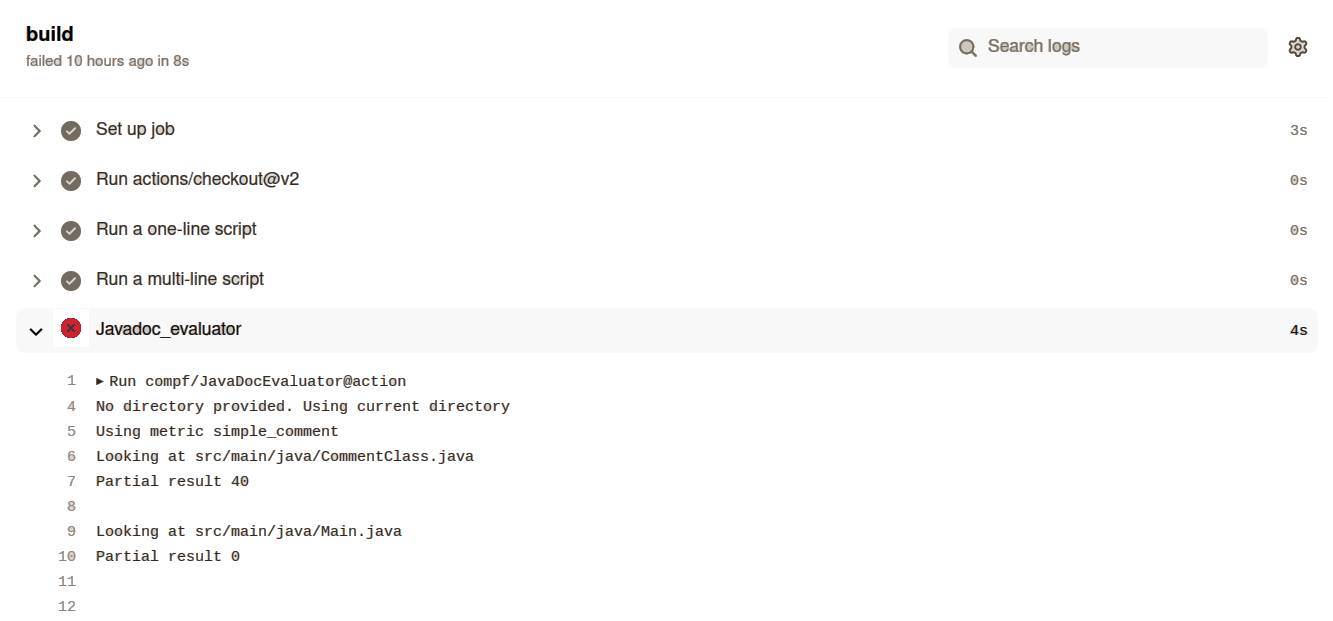
\includegraphics[width=\columnwidth]{figures/chapter2/workflow_output2.png}
    \caption{Ausgabe eines Workflows}
    \label{fig:workflow_output}
\end{figure}

\subsubsection{Erstellung einer eigenen Action}
Um eine eigene GitHub Action zu erstellen, muss in dem Hauptverzeichnis des Repositorys, in dem der Programmcode der Action liegt, eine Datei namens \enquote{action.yaml} oder \enquote{action.yml} erstellt werden. Listing \ref{lst:create_action_example} zeigt eine beispielhafte \enquote{action.yaml}.
	\begin{figure}[h!]
			\lstinputlisting
			[caption={Beispielhafte Action-Konfigurationsdatei},
			label={lst:create_action_example},
			captionpos=b, basicstyle=\footnotesize, tabsize=1, showstringspaces=false,  numbers=left,language=YAML]
			{figures/chapter2/create_action_example.yaml}
		\end{figure}
Zunächst wird der Name der Action und eine Beschreibung definiert. Anschließend können Eingabeparameter definiert werden, die später im Programm verwendet werden können. Zu jedem Parameter muss auch festgelegt werden, ob er zwingend erforderlich ist und den Standardwert des Parameters. Außerdem können Ausgabeparameter festgelegt werden, die spätere Actions als Eingabe nutzen können. Danach wird festgelegt, wie diese Action ausgeführt wird. Eine Action kann in einer JavaScript-Umgebung, in einem Docker-Container, oder als Liste von verschiedenen Steps ausgeführt werden \cite[S. 117ff.]{github_action_book}. 


\section{Verwandte Werkzeuge}
Um die Qualität der Softwaredokumentation in Javadoc zu bewerten, gibt es bereits einige Programme. In vielen Fällen handelt es sich dabei um Programme, die nicht auf die Bewertung der Softwaredokumentation beschränkt sind, sondern auch andere Fälle von unsauberem Code erkennen können. Da die Bewertung der Dokumentation nicht der primäre Zweck der Programme ist, sind die verwendeten Metriken recht allgemein und erkennen viele Problemfälle nicht. Nichtsdestotrotz sind diese Programme, dadurch dass sie viele \enquote{Code-Smells} erkennen, gut geeignet, um sich ein gutes Bild über die Qualität des Quellcodes zu verschaffen und den Entwickler zu Clean-Code zu motivieren. 
\subsubsection{Checkstyle}
Eines der bekanntesten Programme ist Checkstyle\cite{Checkstyle}. Mit Checkstyle lässt sich beispielsweise prüfen, ob alle Methoden überhaupt ein Javadoc-Block besitzen, der Javadoc-Block korrekt platziert wurde oder ein Javadoc-Tag wie zum Beispiel \enquote{@deprecated} auch mit einer zusätzlichen Begründung versehen wurde. 
\subsubsection{PMD}
Des Weiteren gibt es das Programm PMD \cite{PMD}, das ebenfalls einige Metriken für Javadoc mitliefert. Dazu gehört, ob jede öffentliche Methode dokumentiert wurde oder die Kommentare generell zu lang sind. Interessanterweise gibt es auch die Möglichkeit, bestimmte Wörter, die als anstößig empfunden werden, aus Kommentaren und Dokumentationen auszuschließen, damit Kommentare neutral bleiben. 
\subsubsection{Javadoc}
Das oben erwähnte Javadoc-Tool bietet ebenfalls die Möglichkeit, beim Generieren der HTML-Datei die Qualität des Javadocs zu prüfen. Dabei werden vor allem fehlende Tags für Parameter etc. bemängelt. Zudem erkennt Javadoc auch Tabellen mit fehlender Überschrift und andere Designmängel, die in der HTML-Seite später auffallen. Auch fehlerhaftes HTML kann erkannt werden.

\section{Verwandte Arbeiten}

Neben den praktischen Tools, die den Softwareentwickler bei der Bewertung der Softwaredokumentation unterstützen, wurden auch einige wissenschaftliche Arbeiten veröffentlicht, die sich mit Metriken über Softwaredokumentation auseinandersetzen. 


\subsubsection{Quasoledo}\label{chapter:Quasoledo}
In \cite[S. 4-10]{HowDocumentationEvolvesoverTime} geben die Autoren einige Metriken an, die sie für die Bewertung der Softwaredokumentation als nützlich erachten, und stellen ein Programm namens \textit{Quasoledo} vor, dass mittels dieser Metriken Softwaredokumentationen analysieren kann. Zu den Metriken gehören z.~B.  \textit{ANYJ},  welches den Anteil der dokumentierten Deklarationen an allen Deklarationen beschreibt und \textit{KINCAID}, welches die Lesbarkeit von Texten beschreibt.

Die Arbeit wertet anschließend die Javadoc-Dokumentation von Eclipse aus und findet heraus, dass öffentliche Methoden häufiger dokumentiert sind und ihre Dokumentation oft lesbarer ist. Außerdem wenden die Autoren das Tool auf die gesamte Versionshistorie von Eclipse bis zum 8. April 2006 an und plotten den Verlauf der Dokumentationsqualität über diesem Zeitraum. Dabei wird sichtbar, dass die Qualität am Anfang des Projektes noch sehr stark schwankt, aber nach einiger Zeit recht konstant bleibt. 
\subsubsection{JavaDocMiner}
Eine weitere Arbeit, die eine der Grundlagen dieser Bachelorarbeit ist, ist der \enquote{JavaDocMiner} \cite[S. 68-79]{AutomaticQualityAssessmentofSourceCodeComments:TheJavadocMiner}. In diesem Konferenzpapier wird ein Programm beschrieben, welches mittels einfacher Heuristiken eine Einschätzung der Softwaredokumentation beschrieben. Das Tool extrahiert aus XML-Dateien, die mittels eines selbst geschriebene Doclet aus Javadoc erstellt wurden, die notwendigen Informationen und wendet dann auf diese XML-Struktur die Metriken an. 

Insgesamt verwendeten die Autoren viele Metriken aus dem Tool \hyperref[chapter:Quasoledo]{Quasoledo}, führen aber neue auch Metriken ein, die Anzahl der Abkürzungen zählen, da diese laut der Arbeit vermieden werden sollten. Auch die durchschnittliche Anzahl an Wörtern pro Javadoc-Kommentar wird als Metrik verwendet. 

Anschließend wendeten die Autoren das Tool auf den Quellcode an und prüften, ob es eine Korrelation zwischen der Anzahl an Bugs und der Qualität der Dokumentation nach den benannten Metriken und fanden dabei heraus, dass die Kincaid-Metrik nur wenig mit der Anzahl der Bugs korreliert, während es bei anderen Metriken wie z.~B. \textit{ANYJ} eine starke negative Korrelation gab. 

\subsubsection{Doc2Spec}
Die Autoren in \cite[S. 307ff.]{InferringResourceSpecificationsfromNaturalLanguageAPIDocumentation} stellen ein Tool namens \textit{Doc2Spec} vor und erläutern ein Verfahren, um herauszufinden, ob eine API korrekt verwendet wurde. Dabei werden die Javadoc-Kommentare einer API analysiert und dann mit der Verwendung der API verglichen, um Fehler bei der Handhabung der API zu finden. 

Für jede dokumentierte Methode der API wird ein Aktion-Ressource-Paar erstellt. Diese beschreibt, welche Aktion auf welche Ressource ausgeführt wird. Bei einer Methode namens \textit{close}, die mit dem englischen Text \enquote{Initiates close of the connection handle at the
application level} dokumentiert wird, lässt sich beispielsweise schlussfolgern, dass das Aktion-Ressource-Paar \textit{(close,connection)} sein kann; denn die Aktion \textit{close} bezieht sich auf die Ressource \textit{connection}. Dabei sind aber manchmal mehrere Aktion-Ressource-Paare möglich\cite[S. 308]{InferringResourceSpecificationsfromNaturalLanguageAPIDocumentation}.

Anschließend werden die gefundenen Ressourcen anhand der Klassenhierarchie passend gruppiert. Außerdem werden die Aktionen in fünf Kategorien eingeordnet, in der die meisten Java-Methoden passen. Die Kategorien sind Methoden, die eine Ressource oder Objekt erstellen, eine Ressource sperren, auf eine Ressource zugreifen, eine gesperrte Ressource wieder freigeben und Ressourcen schließen. 

Mit diesen generierten Informationen kann dann bei Quelltext, welches diese API verwendet, geprüft werden, ob die Methoden dieser Ressource in der richtigen Reihenfolge aufgerufen werden. Beispielsweise muss eine Ressource zuerst erzeugt und gesperrt werden, bevor irgendwelche Manipulationen angewendet werden. Außerdem kann geprüft werden, ob eine Ressource auch wieder freigegeben und geschlossen wird, sodass Speicherlecks verhindert werden. Dabei werden alle möglichen Ausführungspfade einer Methode geprüft, da ein fehlendes Freigeben von Ressourcen z.~B. im Ausnahmefall ein häufiger Fehler sein kann. 

\subsubsection{iComment}
Das Programm \textit{iComment}  wurde hauptsächlich für C-Programme entwickelt, um Probleme zwischen der Dokumentation und dem Quellcode zu finden. Dabei konzentriert sich das Programm auf das Finden von Synchronisationsproblemen, die bei Programmen mit mehreren Threads auftauchen können.  Bei einem exklusiven Ausschluss besitzt eine Methode einen sogenannten Lock auf ein Objekt und nur diese Methode darf mit dem Objekt arbeiten.

Setzt nun die Dokumentation einen Lock voraus, aber der Programmierer hat keinen Lock angefordert, können sehr schnelle und subtile Bugs entstehen, die nur schwer findbar sind. \cite[S. 145ff.]{icomment}

Das Programm wurde auf dem Quellcode des Linux-Kernels und Mozilla angewandt und dabei mögliche Bugs gefunden, die später auch von den Entwicklern bestätigt wurden\cite[S. 146.]{icomment}.
\subsubsection{@tComment}\label{@tComment}
Ein anderer Ansatz, der ebenfalls mit Javadoc arbeitet, heißt \enquote{@tComment}\cite[S. 1ff.]{@tComment:TestingJavadocCommentstoDetectComment-CodeInconsistencies}. Dabei wurde die Konsistenz der Javadoc-Dokumentation mit dem tatsächlichen Programmcode verglichen. Anders als die vorherigen Ansätze, wird hier das Programm dynamisch ausgeführt. Dabei werden die verschiedenen Methoden und ihr dazugehörige Javadoc-Dokumentation analysiert und daraus mittels einfacher Heuristiken ermittelt, ob ein  Nullwert für einen Parameter eine Inkonsistenz zwischen Dokumentation und Quellcode offenbart.

Beispielsweise kann die Dokumentation einer Java-Methode beschreiben, dass ein Parameter nicht null sein darf. Daraus kann gefolgert werden, dass ein Nullwert für diesen Parameter zu einer Ausnahme führt. Wenn diese Ausnahme dann auch genauer in der Dokumentation genauer spezifiziert ist, sollte genau diese Ausnahme bei einem Nullwert geworfen werden. 

Falls Nullwerte explizit erlaubt sind, sollte die Methode sich dann stets korrekt verhalten und keine Ausnahmen werfen. 

\enquote{@tComment} kann mit diesen einfachen Regeln jede Methode ausführen und prüfen, ob sich die Methode tatsächlich verhält, wie die Dokumentation es beschreibt. Dabei verwendet das Programm einfache \ac{NLP}-Heuristiken in der englischen Sprache; zum Beispiel prüft das Programm, ob die kurz vor dem Wort \enquote{null} ein negierendes Wort wie \enquote{not} oder \enquote{never} auftaucht und klassifiziert dann den dazugehörigen Parameter als Parameter, der nie null sein darf. 




\chapter{Konzeption}\label{chapter_conception}
Im Folgenden wird ein Konzept für die Implementierung des Tools vorgestellt, das  die Ziele der Bachelorarbeit erfüllen soll.
\section{Traversierung aller relevanten Dateien}\label{chapter:traversing}
Softwareprojekte bestehen aus Hunderten von Dateien, die nicht alle Quellcode enthalten. Beispielsweise gehören Konfigurationsdateien, Ressourcedateien wie Bilder oder binäre Dateien zu den Dateien, bei denen eine Analyse der Softwaredokumentation im Hinblick auf die begrenzte Zeit für die Bachelorarbeit nicht implementierbar ist. Daher ist es sinnvoll, bestimmte Dateien bei der Analyse auszuschließen beziehungsweise nur bestimmte Dateien zu betrachten. Bei einer Weiterentwicklung des Tools nach Abschluss der Bachelorarbeit kann das Tool auf andere Dateitypen ausgeweitet werden, um so ein besseres Gesamtbild über die Softwaredokumentation zu erhalten.

Um die relevanten Dateien zu finden, wird zunächst ein übergeordnetes Verzeichnis benötigt, was bei Softwareprojekten aber der Standard sein sollte. Dieses Verzeichnis kann dann rekursiv durchlaufen werden und somit die Liste aller darin gespeicherten Dateien abgerufen werden. Die relevanten Dateien können dann durch Überprüfung ihres Dateinamens mittels bestimmter Regeln ermittelt werden, die der Benutzer des Tools festlegen kann.

Beim JavadocEvaluator wird hierzu die NPM-Bibliothek Minimatch \footnote{\href{https://github.com/isaacs/minimatch}{Minimatch GitHub-Repository (besucht am 07.01.2022)}} verwendet, die es ermöglicht, Dateinamen mit Wildcard-Patterns zu vergleichen. Zum Beispiel könnte der Dateiname \enquote{test.txt} mit der Wildcard \enquote{test.*} verglichen werden und die Bibliothek würde eine Übereinstimmung melden.

\section{Parsing der Java-Dateien} 
Jede Datei, die relevant sein soll, muss anschließend weiterverarbeitet werden. Für die Bewertung der Dokumentation sind nur wenige Bestandteile relevant. Beispielsweise sind alle For-Schleifen, If-Verzweigungen und viele andere Komponenten in Methodenrümpfen nicht relevant, da diese nur mit normalen Kommentaren und nicht mit Javadoc kommentiert werden; (sie werden dennoch unstrukturiert als Zeichenkette gespeichert, damit Metriken diese Information eventuell nutzen können). Aus diesem Grund müssen die notwendigen Informationen extrahiert werden. Zudem ist es ein Ziel der Arbeit , eine Erweiterbarkeit auf andere objektorientierte Programmiersprachen zu ermöglichen. Daher müssen die Informationen in ein abstraktes Format gebracht werden, welches eine gute Annäherung für die meisten objektorientierten Programmiersprachen ist. Beispielsweise unterscheiden sich die Zugriffsmodifizierer vieler Programmiersprache, sodass eine einheitliche Schnittstelle schwer umsetzbar ist. Daher enthält die abstrakte Repräsentation nur Informationen, ob eine Komponente als öffentlich markiert ist. Dies ist sinnvoll, da öffentliche Komponenten als Teil der öffentlichen Schnittstelle eher dokumentiert werden sollten als nicht öffentliche und eine weitergehende Differenzierung kaum Vorteile bietet. In einigen Programmiersprachen wie z. B. Python gibt es keine expliziten öffentliche Komponenten, jedoch existieren de facto Standards für Bezeichner, sodass beispielsweise private Komponenten zwei Unterstriche als Präfix haben.

Außerdem werden in der abstrakten Repräsentation die Vererbung etwas vereinfacht dargestellt, indem nicht zwischen Basisklassen und Schnittstellen unterschieden wird, da es auch hier Unterschiede zwischen Programmiersprachen gibt, und die Informationen über die Vererbung, falls sie überhaupt von einer Metrik verwendet wird, vermutlich nicht so detailreich sein müsste. Zudem werden Konstruktoren als Methoden mit den Namen \enquote{constructor} und Schnittstellen als Klassen repräsentiert, da auch hier eine zu feine Spezifikation nicht notwendig sein wird.  

  

In anderen Fällen gibt es jedoch viele Gemeinsamkeiten zwischen objektorientierten Programmiersprachen; so gibt es in  allen relevanten Sprachen Klassen, Methoden und Felder, die alle einen Namen haben. Des Weiteren haben Methoden und Felder einen (Rückgabe-)Type und Methoden besitzen Parameter, die ihrerseits durch einen Namen und einen Typen definiert sind. Einige Sprachen sind zwar nicht stark typisiert, jedoch kann für nicht bekannte Datentypen ein Alias wie \enquote{Any} oder  \enquote{Object} verwendet werden.  Zudem sind viele Komponenten hierarchisch; in den meisten Sprachen können beispielsweise Klassen andere Klassen enthalten, sodass diese abstrakte Struktur diese Tatsache berücksichtigen müsste. 

Um dennoch sprachspezifische Funktionen anbieten zu können, besitzt jede Komponente ein Feld mit dem Typen \textit{ComponentMetaInformation}, das wie oben erwähnt die Information enthält, ob eine Komponente als öffentlich angesehen werden soll. Dieser Typ, welches eine Schnittstelle ist, kann von einer Klasse implementiert werden, um Parser für andere Programmiersprachen die Möglichkeit zu geben, zusätzliche sprachspezifische Informationen zu speichern. Beim Java-Parser wird diese Funktion beispielsweise genutzt, um zu speichern welche \enquote{checked} Ausnahmen eine Methode werfen kann, sodass später ein Vergleich mit der Javadoc möglich ist. Die Schnittstelle enthält nur die Anforderung, eine \textit{isPublic}-Methode anzubieten und kann daher für viele andere objektorientierte Programmiersprache Informationen speichern, die für einige Metriken eventuell nützlich sind. 
 \clearpage
 \begin{figure}[ht!]
 \begin{tikzpicture}
 \pgfmathsetlengthmacro\breite{6cm}
\pgfmathsetlengthmacro\hoehe{2.567cm}
\pgfmathsetlengthmacro\InnerSep{0.4cm}
\node[draw,
anchor=center, 
inner sep=0pt, 
minimum width=5cm, text width=6cm-\InnerSep,
align=justify,
minimum height=\hoehe
] (java) {
  \hspace*{0.1cm}\textbf{public} \textbf{class} Main\{.\newline 
     \hspace*{0.5cm}\textbf{private} \textbf{int} test(\textbf{int} a)\{\newline
    \hspace*{0.5cm}\}\newline
\hspace*{0.1cm}\}

};
\node[draw,text width=5.5cm, left = of java](python){
\textbf{class} Main:\newline
     \hspace*{0.5cm}\textbf{def} \_\_test(a:\textbf{int}): -> \textbf{int}\newline
         \hspace*{1cm}pass

};
\draw[line width=0.05cm] (python) -- (-4,-2.5) ;
\draw [line width=0.05cm](java) -- (-4,-2.5);
\draw[->,thick,line width=0.05cm] (-4,-2.5) -- (-4,-3.5);
\draw [] (-9,-3.5) rectangle(4,-16);
\begin{scope} {0,-10}
       \begin{object}[text width=8cm]{fileObj}{-4,-4}
        \instanceOf{FileComponent}
        \attribute{name = "filepath"}
        \attribute{parent = null}
        \attribute{children={[}classObj{]}}
      \end{object}
      \begin{object}[text width=8cm]{classObj}{-4,-8 }
        \instanceOf{ClassComponent}
        \attribute{name="Main"}
        \attribute{parent=fileObj}
        \attribute{children={[}methodObj{]}}
          \attribute{metaInformation=meta}
      \end{object}
    \begin{object}[text width=8cm]{methodObj}{-4,-12}
        \instanceOf{MethodComponent}
        \attribute{name="test"}
        \attribute{parent=classObj}
        \attribute{params={[}paramsObj{]}}
        \attribute{metaInformation=meta2}
        \attribute{returnType=int}
      \end{object}
      \begin{object}[text width=2.5cm]{paramObj}{2,-10}
        \attribute{name=a}
        \attribute{type=int}
      \end{object}
    \begin{object}[text width=2.5cm]{meta}{2,-6}
        \attribute{isPublic=true}
      \end{object}
    \begin{object}[text width=2.5cm]{meta2}{2.5,-14.5}
        \attribute{isPublic=false}
      \end{object}
\end{scope}
\begin{scope}[line width=0.05cm]
    \aggregation{fileObj}{}{}{classObj}{}{}
     \aggregation {classObj}{}{}{methodObj}{}{}
      \aggregation {methodObj}{}{}{paramObj}{}{}
    \aggregation {classObj}{}{}{meta}{}{}
        \aggregation {methodObj}{}{}{meta2}{}{}
\end{scope}

    
\end{tikzpicture}
     
     \caption{Objektdiagramm aus Java- und Python-Code}
     \label{fig:python_java_comp}
 \end{figure}


Abbildung \ref{fig:python_java_comp} veranschaulicht wie eine einfache Datei in die Objektstruktur umgewandelt werden kann. Dabei wird ein einfache Java-Klasse und eine semantisch äquivalente Python-Datei als Beispiel verwendet, um zu zeigen, dass aus beiden Sprachen eine gleiche Objektstruktur erzeugt werden kann. Dabei wurden zur Übersichtlichkeit einige nicht relevanten Attribute entfernt.

Das Programm in beiden Sprachen besteht aus einer öffentlichen Klasse \textit{Main} und einer privaten Methode \textit{test}, die einen Parameter \textit{a} als Ganzzahl erhält und eine Ganzzahl zurückgibt. Die höchste Hierarchieebene ist immer ein \textit{FileComponent}. Diese Datei enthält hier genau ein Kind namens \textit{classObj}, könnte aber in anderen Fällen auch mehrere Kinder (wie z.~B. Klassen enthalten). Die Klasse besitzt zudem einen Verweis auf ihren Elternteil. Außerdem enthält das \textit{classObj} eine Referenz auf MetaInformationen, die hier nur angeben, dass die Klasse öffentlich ist. In diesen MetaInformationen könnte auch die Basisklasse und andere relativ sprachspezifische Informationen enthalten. Die Klasse enthält wiederum genau die Methode als einziges Kind. Die Methode hat ebenfalls einen Verweis auf Metainformation, welche die Methode als privat markieren. Außerdem hat die Methode einen \textit{returnType} und einen Verweis auf die Liste der Parameter, die wiederum aus einen Namen und einen Datentyp bestehen.


\section{Konzeption der Metriken}
Nachdem eine Datei in ihre einzelnen Komponenten zerlegt wurde, kann die Qualität der Softwaredokumentation überprüft werden. Jede gefundene Komponente besitzt einen Verweis auf die dazugehörige Dokumentation, die bei Nichtvorhandensein auch null sein kann. Anhand dieser Referenz kann geprüft werden, ob die Softwaredokumentation der Komponente ausreichend ist. Zur Bewertung der Dokumentation gibt es verschiedene  Möglichkeiten. Beispielsweise könnte überprüft werden, ob eine Komponente dokumentiert oder undokumentiert ist. Eine weitere Möglichkeit wäre es die Verständlichkeit der Dokumentation zu prüfen. Jedes dieser Vorgehen basiert auf eine Metrik, die auf wissenschaftliche Studien beruht oder zumindest plausibel ist. In diesem Abschnitt wird ein Konzept erläutert, um eine Metrik zu implementieren. Anschließend wird beschrieben, wie die Ergebnisse jeder Metrik zusammengefasst werden, um ein Endresultat zu erhalten. 

\subsection{Implementation einer Metrik}\label{chapter:metric_impl}
Damit eine Metrik die Dokumentation bewerten kann, benötigt sie Zugriff auf die Komponente. Außerdem muss sie ihr Ergebnis irgendwie veröffentlichen bzw. zwischenspeichern, damit es später weiterverarbeitet werden kann. Des Weiteren ist nicht jede Metrik mit jede Komponente kompatibel. Eine Metrik, die überprüft, ob jeder Methodenparameter dokumentiert ist (vgl. Kapitel \ref{chapter:method_doc}), kann mit anderen Komponentenarten weniger anfangen. Zudem sollte es die Möglichkeit geben, das Verhalten einer Metrik mittels Parameter anzupassen, damit die Metrik konfigurierbar bleibt. Zuletzt sollte eine Metrik bei der Bewertung auch begründen, warum die Dokumentation einer Komponente nicht ausreichend ist.

Eine Möglichkeit, diese Anforderung für eine Metrik umzusetzen, wäre die Verwendung einer Methode pro Metrik, welche die Komponente und die Parameter als Eingabe erhält und daraus die Bewertung und eventuelle Begründung ermittelt und zurückgibt. Allerdings ist dieser Ansatz sehr prozedural; es gibt beispielsweise keine Kapselung zwischen den Metriken.  

Ein anderer Ansatz, der hier auch gewählt wird, ist es, jede gewünschte Metrik als Klasse zu implementieren. Jede implementierte Metrik kann somit die notwendigen Berechnungen abgekapselt von anderen Metriken erledigen, was die Wartbarkeit verbessert. Um trotzdem für eine einheitliche Schnittstelle zu sorgen, muss jede zu implementierende Metrik von einer abstrakten Basisklasse \textit{(DocumentationAnalysisMetric)} erben,, welche die Implementation bestimmter Methoden vorschreibt, sodass ein Benutzer der Metrik auch ohne Wissen über die Interna der Metrik diese verwenden kann. Die Methode \textit{shallConsider} überprüft, ob eine Komponente für diese Metrik ist geeignet ist und gibt dementsprechend einen Wahrheitswert zurück. Die Methode \textit{analyze} führt anschließend die Bewertung durch.

Zudem kann ein Objekt, das eine Metrik repräsentiert und daher von \textit{DocumentationAnalysisMetric} erbt (Metrikobjekt), Parameter besitzen, welche spezifische Eigenschaften der Metrik modifizieren kann. Diese Eigenschaft werden sehr abhängig von der Metrik sein, sodass eine einheitliche Schnittstelle nur schwer umsetzbar ist. Daher werden die Parameter als Datentyp \textit{any} übergeben, sodass es keine Typüberprüfung gibt. Alternativ wäre eine assoziative Liste möglich, bei dem ein Parametername als Zeichenketter ein Wert zugeordnet wird, aber auch hier könnte kein Überprüfung eines Datentypes vorgenommen werden. 

Eine  weitere Voraussetzung für ein Metrikobjekt ist ein eindeutiger Name. Dadurch kann die gleiche Metrik mit unterschiedlichen Parametern verwendet werden. Außerdem wird so eine Zuordnung von Gewichten vereinfacht. Standardmäßig besteht dieser eindeutige Name aus dem Namen der implementierten Metrik gefolgt von einem Unterstrich und einer fortlaufenden Nummer.
\subsubsection{Bewertung der Dokumentation}
Die Methode \textit{analyze} muss eine Bewertung darüber abgeben, ob die Qualität der Dokumentation ausreichend ist. Für die Repräsentation dieser Bewertung gibt es viele Möglichkeiten, allerdings ist eine numerische Bewertung mittels einer Intervallskala am sinnvollsten, da so der arithmetische Mittelwert, der Median etc. berechnet werden kann, was für die Bildung des Gesamtergebnisses wichtig ist.
Die numerische Bewertung soll eine Aussage über die Dokumentationsqualität liefern. Eine Bewertung von 0 steht für eine sehr schlechte bis nicht existente Dokumentation und die Bewertung 100 steht für eine exzellente Dokumentation, sodass die Bewertung sich als Prozent lesen lassen kann. Das Ergebnis einer implementierten Metrik sollte diesen Wertebereich nicht verlassen, da eine Fehlerbehandlung nicht implementiert ist. Bei Metriken, die per Design schon eine prozentualen Wert zurückgeben (z.~B. \ref{chapter:metrics_simple_comment}) wird diese Vorgabe stets eingehalten. Bei anderen Metriken (z.~B. \ref{chapter:metrics_flesh}) sollte eine mathematische Funktion gefunden werden, die das Ergebnis der Metrik auf den Wertebereich 0 bis 100 abbildet. Die genaue Umsetzung hängt von der Metrik ab. In jedem Falle sollte es für eine Metrik Ergebnisse geben, die auf eine gute bzw. schlechte Dokumentation hindeuten, damit diese auf 100 bzw. 0 abgebildet werden können. Nur durch diese Einschränkung auf einen fixen Wertebereich ist es möglich, den Mittelwert, Median etc. zu bilden und so eine Vergleichbarkeit zu ermöglichen. 

\subsection{Ergebnis der Metrik verarbeiten}

Das berechnete Ergebnis einer Komponente muss nun gespeichert werden, damit es später ausgewertet werden kann. Dazu wird ein \textit{MetricResult}-Objekt erstellt, welches das im vorherigen Unterabschnitt berechnet Ergebnis enthält. Außerdem werden hier eventuelle Begründungen und Hinweise gespeichert, die dem Anwender dabei unterstützen, die Qualität der Dokumentation zu verbessern. Jede Begründung enthält den Dateipfad der betroffenen Datei, die bemängelte Komponente und die Zeilennummer, sodass der Benutzer die problematische Stelle schnell finden kann. Zuletzt wird außerdem eine Zeichenkette gespeichert, die später für die Gewichtung relevant ist. 

Für die Speicherung des Objekt gibt es zwei Möglichkeiten. Die erste Möglichkeit wäre es, dass die \textit{analyze}-Methode das \textit{MetricResult}-Objekt einfach zurückgibt, sodass der Aufrufer damit arbeiten kann. Bei der zweiten Möglichkeit wird das Ergebnis einem anderen Objekt übergeben, der dann die Weiterverarbeitung vornimmt. Dies hat den Vorteil, dass eine Metrik kein Ergebnis zurückliefern muss, wenn es kein sinnvolles Ergebnis berechnen kann. Bei einem Rückgabewert müsste dann ein ungültiger Wert wie z.~B. \textit{null} vereinbart werden. Außerdem kann eine Metrik auch mehrere Resultate speichern, was bei komplexeren Komponenten interessant sein dürfte. Dieses weitere Objekt ist ein  \textit{MetricResultBuilder}, der wie in nächsten Unterabschnitt beschrieben, die Softwaredokumentationsqualität jeder Komponente sammelt und daraus ein Gesamtergebnis berechnet.  
\subsection{Resultate der Metriken anwenden}
Da in einer Datei mehrere Komponenten durchaus Standard sind (eine Klasse mit einer enthaltener Methode zählt bspw. als zwei Komponenten), müssen die Bewertungen jeder Komponente passend aggregiert werden. Dazu wird dem \textit{MetricResultBuilder} jedes Ergebnis mittels der \textit{processResult}-Methode mitgeteilt, welches das Ergebnis in einer Liste speichert. Wenn alle Metriken verarbeitet sind, wird daraus ein Gesamtresultat gebildet. Dies geschieht durch die Methode \textit{getAggregratedResult}. Dabei wird standardmäßig ein arithmetischer Mittelwert gebildet. Durch Ableitung kann diese Methode überschrieben werden, um den Median oder eine Gewichtung bei der Bildung des Gesamtergebnisses zu verwenden  sodass die Wahl des Algorithmus flexibel bleibt . Ein \textit{ResultBuilder} basiert auf dem Vorbild des Design-Patterns \enquote{Builder} aus \cite[S.139-149]{gamma2015design}, da es aus einzelnen Metrikresultaten ein vollständiges Metrikergebnis baut.

Abbildung \ref{fig:metrics_apply} zeigt schematisch, wie aus verschiedenen Dateien ein Gesamtergebnis ausgebaut wird. Hier werden zwei Dateien und zwei exemplarische Metriken verwendet. Links unten wird die erste Datei (rot) durch der ersten Metrik bewertet. Dazu wird ein interner \textit{MetricResultBuilder} verwendet, was aber hier aus Übersichtlichkeitsgründen nicht dargestellt wird. Auch die zweite Metrik bewertet die gleiche Datei, sodass von beiden Metriken ein Ergebnis vorliegt. Diese Ergebnisse werden von einem \textit{MetricResultBuilder} verarbeiten, der beispielsweise die Ergebnisse je nach Metrik gewichten kann. Das Ergebnis dieses Vorgangs wird von einem separaten \textit{MetricResultBuilder} verarbeitet, welcher dieses und das Ergebnis der zweiten Datei (grün), das analog ermittelt wird, verarbeitet und und eine Gewichtung nach Dateipfad vornehmen könnte. Das Gesamtergebnis oben in der Mitte ist dann Maß für die Entscheidung, ob die Dokumentationsqualität als ausreichend angesehen wird. 
\begin{figure}[ht!]
\fontsize{7}{10}\selectfont
    \centering
\includesvg[scale=0.5]{figures/chapter3/metrics.svg}
    \caption{Anwendung der Metriken}
    \label{fig:metrics_apply}
\end{figure}
 
\subsection{Zuordnung der Gewichte}\label{chapter_weights_assign}
Für einige Algorithmen muss eine Gewichtung vorgenommen werden, um bestimmte Ergebnisse besser oder schlechter zu bewerten. Dazu muss jedes Teilergebnis eine Gewicht zugeordnet werden. Ein Teilergebnis, das gewichtet werden soll, kann hier entweder von einer einzelnen Metrik oder einer einzelnen Datei produziert werden. Im Falle einer Datei existiert durch den Dateipfad ein eindeutiger Name. Auch bei einer Metrik wird dies durch die Konzeption in Kapitel \ref{chapter:metric_impl} sichergestellt. Die Zuordnung erfolgt über einen \textit{WeightResolver}, welches eine Schnittstelle anbietet, um einen Bezeichner auf ein Gewicht abzubilden. Bei dem eindeutigen Namen eines Metrikobjektes kann hierfür eine assoziative Liste verwendet werden. 
Für Dateipfade ist dies allerdings nicht praktikabel, da es eine Vielzahl an Dateien geben kann. Stattdessen werden hier ähnlich wie bei der Filterung von Dateien in Kapitel \ref{chapter:traversing} Wildcard-Patterns verwendet. Eine assoziative Liste speichert dazu jedes Wildcard-Patterns und das dazugehörige Gewicht. Bei einer Abfrage kann das Gewicht des ersten Eintrages zurückgegeben werden, bei dem der Dateipfad mit dem Wildcard-Patterns kompatibel ist. Dies ermöglicht es, ganze Verzeichnisse oder Dateien mit bestimmten Namen stärker zu gewichten. Für eine Datei, bei dem kein Wildcard-Pattern zutrifft, wird ein standardmäßiges Gewicht (z.~B. 1) zurückgegeben. 

Jedes \textit{MetricResult}-Objekt enthält eine Zeichenkette, die den Erzeuger des Ergebnisses repräsentiert; so kann jedes Einzelresultat passend gewichtet werden. Bei der Bildung eines Gesamtergebnis aus einzelnen Teilresultaten mittels der Methode \textit{getAggregatedResult} muss das neue \textit{MetricResult}-Objekt ebenfalls ein Erzeuger besitzen. Dieser Erzeuger wird vom Anwender der Funktion übergeben. Werden beispielsweise die Ergebnisse mehrere Metriken aber einer Datei zusammengefasst, so ist der neue Erzeuger der Dateipfad. Bei dem endgültigen Gesamtergebnis ist eine Gewichtung nicht mehr sinnvoll, daher kann dann eine leere Zeichenkette übergeben werden.

\subsection{Implementierte Algorithmen zur Bildung eines Gesamtergebnisses}
In den folgenden Unterabschnitten wird jeder Algorithmus, welches ein Gesamtresultat bildet, kurz erläutert und dabei kurz auf die Vor- und Nachteile eingegangen. 

\subsubsection{Arithmetischer Mittelwert}
Der arithmetische Mittelwert wird bereits durch die Klasse \textit{MetricResultBuilder} implementiert. Dieser Algorithmus berücksichtigt jedes Ergebnis gleichermaßen. Dies ist insbesondere für die Aggregierung der Ergebnisse der einzelnen Dateien sinnvoll, da jede Datei gleich behandelt werden sollte und eine Gewichtung von möglicherweise Tausenden von Dateien nur schwer umsetzbar ist. Es sollte allerdings auch beachtet werden, dass der Mittelwert extreme Ausreißer berücksichtigt. Dies ist hier manchmal sinnvoll, da sehr schlechte Dokumentation besser berücksichtigt wird und so ein verlässliches Gesamtergebnis geliefert wird.


\subsubsection{Median}
Der Median der Einzelresultate wird von der Klasse \textit{MedianResultBuilder} berechnet. Dabei werden die Einzelresultate nach den bekannten Median-Algorithmus verarbeitet. Bei einer geraden Anzahl an Elementen wird der Median aus dem Mittelwert der zwei infrage kommenden Ergebnissen gebildet. 

Der Median berücksichtigt einzelne Ausreißer nicht und kann daher interessant sein, wenn ein allgemeines Bild von der Dokumentationsqualität erhalten werden soll. Es sollte aber beachtet werden, dass die Anwendung des Medians ein Sortiervorgang benötigt, der in den meisten Fällen eine Komplexität von $O(n*log(n))$ hat. Bei der überschaubaren Anzahl an Metriken wird dies weniger relevant sein, bei einer Anwendung des Medians auf vielen Dateien durchaus wohl.


\subsubsection{Gewichteter Mittelwert}
Der gewichtete Mittelwert ist in der Klasse \textit{WeightedMetricResultBuilder} implementiert. Die Zuweisung der Gewichte erfolgt wie in Kapitel \ref{chapter_weights_assign} beschrieben durch einen \textit{WeightResolver}. Die Gewichte müssen nicht normiert werden, da dies während der Berechnung implizit erledigt wird. Die Resultate jeder Metrik werden multipliziert mit dessen Gewicht, dann aufsummiert und zuletzt durch die Summe aller Gewichte geteilt. 


Dieser Algorithmus ermöglicht es, bestimmte Metriken zu bevorzugen bzw. zu benachteiligen. Dies ist sinnvoll, da nicht jede Metrik immer ein aussagekräftiges Ergebnis liefert und bestimmte Metriken je nach Situation ein besseres Bild über die Dokumentationsqualität liefern. Allerdings ist auch zu beachten, dass die Wahl der Gewichte nicht trivial ist und ein Vergleich von Ergebnissen, die verschiedene Gewichte verwenden, nicht sinnvoll ist.

\subsubsection{Gewichteter Median}
Der gewichtete Median wurde leicht abweichend nach \cite[S. 37]{YAGER199835} implementiert. Dabei wird zunächst die Summe der Gewichte berechnet und die Resultate nach ihrem Gewicht sortiert. Anschließend werden die sortierten Resultate und ihre Gewichte so lange aufsummiert, bis diese temporäre Summe die Hälfte der Gesamtsumme überschreitet. Das Metrikergebnis, bei der diese Bedingung zutrifft, ist das gesuchte Gesamtergebnis. Die Vor- und Nachteile dieses Algorithmus entsprechen den Vor- und Nachteilen des gewichteten Mittelwerts und des Medians. So muss auch hier eine Sortierung durchgeführt werden und die Wahl der richtigen Gewichte ist nicht trivial. 
\subsection{Sprachspezifische Informationen für Metriken}
Da das Tool für möglichst viele objektorientierte Programmiersprachen konzipiert werden soll, muss eine Generalisierung erfolgen, da jede Sprache ihre Eigenheiten hat und möglicherweise besondere Funktionen anbietet, die nur schwer in einem abstrakten Format zu bringen sind.

Nichtsdestotrotz können solche sprachspezifischen Eigenheiten auch in der Dokumentation erwähnt werden. daher ist es eine sinnvolle Idee, dass Metriken auch diese Informationen, um ein genaueres Bild der Dokumentationsqualität zu nutzen, ohne jedoch zu wissen, welche Programmiersprache gerade analysiert wird. Beispielsweise können die Checked-Ausnahmen in Java mit den Informationen in der Javadoc verglichen werden. Des Weiteren können. Komponenten einer Schnittstelle oder abstrakten Klasse, die es nicht jeder Programmiersprache gibt, stärker geprüft werden und bei mangelhafter Dokumentation stärker gewichtet werden, da dort die Erfüllung eines Vertrages wichtig ist und daher eine gute Dokumentation wichtiger ist. Auch eine feinere Abstufung je nach Zugriffsmodifizierer einer Komponente wäre so möglich, sodass eine undokumentierte öffentliche Komponente schelchter bewertet wird, als eine Komponente mit dem Zugriffsmodifizierer  \textit{protected}. 

Um solche sprachspezifischen Analysen zu erlauben, besitzt jede Metrik Zugriff auf ein Objekt der Klasse \textit{LanguageSpecificHelper}. Wenn eine neue Programmiersprache hinzugefügt werden soll, kann von dieser geerbt werden. In der Klasse \textit{LanguageSpecificHelper} sidn bereits einige Methoden definiert, die einigen Metriken bei der Bewertung helfen. So bewertet die Methode \textit{rateDocumentationCompatibility}, ob die Dokumentation alle sprachspezifischen Informationen erläutert (z.~B. \textit{@throws}). Die Methode \textit{shallConsider} kann genutzt werden, um überschriebene Methoden zu ignorieren. 

Um eigene Methoden hinzuzufügen, muss diese in der Basisklasse definiert werden. Diese Methode sollte in der Basisklasse keine Aktionen durchführen, sondern entweder gar nichts tun oder Rückgabewerte haben, die keinen Einfluss auf Metriken haben. Anschließend kann diese Methode in einer sprachspezifischen abgeleiteten Klasse der Basisklasse korrekt implementiert werden. Die entsprechende Methode kann dann durch Änderung des Quellcodes der Metrik an den passenden Stellen von der Metrik verwendet werden. So kann beispielsweise das Resultat einer Metrik modifiziert werden oder weitere Ergebnisse mittels des \textit{MetricResultBuilder} angefügt werden. 

\subsection{Ignorieren bestimmter Kommentare}

Unter Umständen kann es sinnvoll sein, bestimmte Komponenten bei der Bewertung auszulassen, weil sie beispielsweise noch nicht vollständig implementiert sind, in einer nicht-englischen Sprache dokumentiert sind oder ein anderer gewichtiger Grund existiert. Für diesen Fall kann die allgemeine Beschreibung der Dokumentation einer Komponente  den Begriff \enquote{\%ignore\_this\% } oder \enquote{\%ignore\_node\%} enthalten. Bei Ersterem wird nur diese Komponente ignoriert und als nicht existent betrachtet. Bei Zweiterem werden sowohl diese Komponente als auch alle Kinder dieser Komponente ignoriert, sofern sie existieren



\begingroup
\renewcommand{\cleardoublepage}{} % TODO maybe removing this and next
\renewcommand{\clearpage}{}
\chapter{Umsetzung}\label{chapter:program}
\endgroup
In diesem Kapitel wird auf die Umsetzung der in Kapitel \ref{chapter_conception} beschriebenen Architektur eingegangen. Dazu werden Informationen über die Einrichtung und Konfiguration des Tools gegeben. Außerdem wird erläutert, wie das Tool konkret Java-Dateien verarbeitet. Zuletzt werden die implementierten Metriken und Algorithmen präsentiert. 
\section{Ausführung des Programms}
In diesem Unterabschnitt wird beschrieben, wie das Programm die in Kapitel \ref{chapter_conception}
beschriebenen Arbeitspakete nutzt, um die Qualität der Softwaredokumentation zu bewerten. 

Die Koordination des Programms wird in der Datei \enquote{index.ts} durchgeführt, die als Einstiegspunkt des Programms verstanden werden kann. In dieser Datei werden die einzelnen Module des Programms in der richtigen Reihenfolge aufgerufen und die Ergebnisse eines Moduls werden durch die \enquote{index.ts}-Datei an das folgende Modul/Arbeitspaket übergeben, soweit sie dort benötigt werden. Dadurch sind die Module voneinander entkoppelt und greifen nicht direkt aufeinander zu. 

Im ersten Schritt  muss die Konfiguration des Programms geladen werden. Dazu wird das Arbeitsverzeichnis von der Kommandozeile gelesen. Basierend auf das Arbeitsverzeichnis kann dann die Konfiguration des Tools geladen werden, wie es in Kapitel \ref{chapter:conf} beschrieben ist.  

Anschließend müssen einige Objekte  initialisiert werden. Hierzu werden die Werte aus der Konfiguration (z.~B. der Konfigurationsdatei) verwendet. Beispielsweise kann durch \textit{builder} der Algorithmus festgelegt werden, der die Einzelergebnisse der einzelnen Metriken zu einem Gesamtresultat kombiniert. Dazu wird das Factory-Pattern verwendet, da damit die Konstruktion eines Objektes aus einer Zeichenkette möglich ist und somit der Anwender in der Konfiguration nur eine bestimmte Zeichenkette oder ID zur Konstruktion eines komplexeren Objektes angeben muss \cite[S. 149-161]{gamma2015design}. Zudem werden die Metriken, die zur Analyse verwendet werden sollen, durch den Metrikmanager registriert.

Außerdem wird eine assoziative Liste für die Dateien und die Metriken erstellt, die den eindeutigen Metriknamen bzw. ein Wildcard-Pattern einer Datei ein Gewicht zugeordnet. Damit kann ein entsprechender \textit{MetricResultBuilder} erzeugt werden. Falls dieser keine Gewichtung benötigt, werden diese Informationen ignoriert. 

Danach müssen die relevanten Dateien gefunden werden. Dazu werden dem Traversierer (siehe Kapitel \ref{chapter:traversing}) die Wildcard-Patterns der zu inkludierenden Dateien und der auszuschließenden Dateien übergeben. Mit der Methode \textit{getRelevantFiles} werden dann alle notwendigen Dateien zurückgegeben.

In nächsten Schritt muss jede Datei mit jeder Metrik geprüft werden und die Ergebnisse gesammelt werden. Hierzu wird eine verschachtelte For-Schleife verwendet. Dabei gibt es zwei Möglichkeiten zur Verschachtelung. Im ersten Fall könnte in der äußeren Schleife jede Datei und in der inneren jede Metrik durchlaufen werden. Alternativ könnte auch die innere und äußere Schleife vertauscht werden. Der erste Ansatz hat den Vorteil, dass jede Datei nur einmal geladen werden muss, was einen Geschwindigkeitsvorteil bringen kann, deshalb wurde dieses Verfahren auch gewählt. Pro Iteration der inneren Schleife wird die aktuelle Datei analysiert und alle gefundenen Metrikresultate, die von den einzelnen Komponenten der Datei stammen, zu einem \textit{MetricResultBuilder} hinzugefügt.

Nach Abschluss der beiden Schleifen steht das Ergebnis durch Aggregation der Resultate in dem \textit{MetricResultBuilder} zur Verfügung und kann genutzt werden, um die Qualität der Dokumentation mit dem Grenzwert bzw. den letzten Wert zu vergleichen. 

\section{Traversierung aller relevanten Dateien und der Komponenten}\label{chapter:traversing}
Softwareprojekte bestehen aus Hunderten von Dateien, die nicht alle Quellcode enthalten. Beispielsweise gehören Konfigurationsdateien, Ressourcendateien wie Bilder oder binäre Dateien zu den Dateien, bei denen eine Analyse der Softwaredokumentation im Hinblick auf die begrenzte Zeit für die Bachelorarbeit nicht implementierbar ist. Daher ist es sinnvoll, bestimmte Dateien bei der Analyse auszuschließen beziehungsweise nur bestimmte Dateien zu betrachten. Bei einer Weiterentwicklung des Tools nach Abschluss der Bachelorarbeit kann das Tool auf andere Dateitypen ausgeweitet werden, um so ein besseres Gesamtbild über die Softwaredokumentation zu erhalten.

Um die relevanten Dateien zu finden, wird zunächst ein übergeordnetes Verzeichnis benötigt, was bei Softwareprojekten aber der Standard sein sollte. Dieses Verzeichnis kann dann rekursiv durchlaufen werden und somit die Liste aller darin gespeicherten Dateien abgerufen werden. Die relevanten Dateien können dann durch Überprüfung ihres Dateinamens mittels bestimmter Regeln ermittelt werden, die der Benutzer des Tools festlegen kann.

Beim \textit{DocEvaluator} wird hierzu die NPM-Bibliothek Minimatch \cite{Minimatch} verwendet, die es ermöglicht, Dateinamen mit Wildcard-Patterns zu vergleichen. Zum Beispiel könnte der Dateiname \enquote{test.txt} mit der Wildcard \enquote{test.*} verglichen werden und die Bibliothek würde eine Übereinstimmung melden.

Auch die Komponenten einer Datei müssen traversiert werden, damit bei jeder Komponente die Dokumentation überprüft werden kann. Da die Komponenten wie in Kapitel \ref{chapter:parsing} beschrieben rekursiv aufgebaut sind, kann dies mittels einer Tiefensuche durchgeführt werden.

\subsubsection{Ignorieren bestimmter Kommentare}

Unter Umständen kann es sinnvoll sein, bestimmte Komponenten bei der Bewertung auszulassen, weil sie beispielsweise noch nicht vollständig implementiert sind, in einer nicht-englischen Sprache dokumentiert sind oder ein anderer gewichtiger Grund existiert. Für diesen Fall kann die allgemeine Beschreibung der Dokumentation einer Komponente  den Begriff \enquote{\%ignore\_this\%} oder \enquote{\%ignore\_node\%} enthalten. Bei Ersterem wird nur diese Komponente ignoriert und als nicht existent betrachtet. Bei Zweiterem werden sowohl diese Komponente als auch alle Kinder dieser Komponente ignoriert, sofern sie existieren.


\section{ANTLR4}
Um die Java-Dateien zu parsen, wird die Bibliothek ANTLR4 \cite{ANTLR} verwendet, die kostenlos verfügbar ist. Diese Bibliothek kann nicht nur viele Programmiersprachen, sondern auch selbst geschriebene Sprachen parsen, sofern eine passende Grammatik verfügbar ist. Daneben gibt es noch Bibliotheken wie Bison oder PEG.JS, die ebenfalls eine ähnliche Aufgabe erfüllen können. Allerdings gibt es bereits vordefinierte Grammatiken für ANTLR4, sodass ein erheblicher Aufwand gespart werden konnte.  

Eine andere Möglichkeit zum Parsen der Java-Dateien ist die NPM-Bibliothek \enquote{java-parser} \cite{Java-parser}. Dies hätte den Vorteil, dass das Parsen, welches nicht der Hauptfokus dieser Bachelorarbeit ist, ausgelagert wird und so Fehler vermieden werden. Allerdings kann diese Bibliothek nicht die Verbindung zwischen einer Komponente und der dazugehörigen Javadoc herstellen, sodass eine Benutzung dieser Bibliothek die Arbeit deutlich erschwert hätte. Daher fiel die Wahl auf \textit{ANTLR4}. Außerdem besteht die Möglichkeit, eine eigene Grammatik für Java zu schreiben, da die originale Grammatik für Java sämtliche Kommentare ignoriert. Da dies jedoch deutlich komplizierter war als erwartet, wird die von vielen Entwicklern geschriebene Grammatik verwendet.

\subsection{Lexer und Parser}
Eine Grammatik für Programmiersprachen besteht immer aus einer Lexer-Grammatik und eine Parser-Grammatik, die jeweils vom Lexer bzw. Parser in dieser Reihenfolge verarbeitet werden, um so eine Baumstruktur einer Quellcodedatei zu erhalten. Der Lexer erstellt aus einer Quellcodedatei eine Liste von Tokens. Dabei ist ein Token eine Gruppierung von einem oder mehreren Zeichen, die eine weitergehende Bedeutung haben. Beispielsweise können Schlüsselwörter einer Programmiersprache oder Operatoren als Token klassifiziert werden. Diese Tokens sind grundsätzlich kontextunabhängig, das heißt für die gleiche Zeichenkette wird das gleiche Token verwendet. Jeder Token wird durch seine Zeichenkette und den Tokentyp klassifiziert.

Listing \ref{lst:lexer_example} zeigt zur Verdeutlichung der Syntax eine Zeile aus der Lexer-Grammatik. 
		\begin{figure} [htbp]
			\lstinputlisting
			[caption={Beispielhafte Syntax vom Lexer},
			label={lst:lexer_example},
			captionpos=b, basicstyle=\footnotesize, tabsize=2, showstringspaces=false,  numbers=left,language=ANTLR]
			{figures/chapter4/lexer_example.g4}
		\end{figure}

Eine Zeile in der Lexer-Grammatik beginnt mit den Namen eines Tokens, gefolgt von einem Doppelpunkt und dann einem regulären Ausdruck, der dieses Token beschreibt. In der beispielhaften Lexer-Grammatik wird ein Javadoc-Kommentar definiert, das mit \enquote{/**} beginnt, dann folgen beliebige Zeichen und endet mit \enquote{*/}. Per Konvention haben die Bezeichner der Tokens nur Großbuchstaben, sie müssen auf jeden Fall mit einem Großbuchstaben beginnen \cite[S. 3]{ANTLR:APredicated-<i>LLk</i>ParserGenerator}. 

Der nächste Schritt ist das  Parsen. Dabei werden die im vorherigen Schritt generierten Tokens, die als Liste vorliegen, genommen und in eine hierarchische Baumstruktur umgewandelt, wobei hier der Kontext die entscheidende Rolle spielt. ANTLR4 lädt ein Token nach dem anderen und prüft, ob es, basierend auf der aktuellen Position in der Baumstruktur, eine Regel gibt, die durch dieses Token erfüllt wird. Wenn es mehrere mögliche Pfade gibt, lädt ANTLR4 so viele Tokens, bis die nächste Regel eindeutig feststeht. Gibt es dennoch Uneindeutigkeiten, so wird die Regel genommen, die als Erstes in der Parser-Datei geschrieben wurde \cite[S. 10ff.]{TheDefinitiveANTLR4Reference}.

So kann eine vereinfachte Parser-Grammatik für Java einen Baumknoten definieren, der eine generelle Methode beschreibt. Eine Methode besteht aus Rückgabetyp, Bezeichner und Parameterliste. Die Parameterliste kann dann als eine Liste von Datentyp-Bezeichner-Paare aufgelöst werden. Der Rückgabetyp einer Methode ist allerdings anders zu verstehen als der Datentyp eines Parameters, da jeder Datentyp eines Parameters auch ein gültiger Rückgabetyp ist, was jedoch nicht umgekehrt der Fall ist; so ist \textit{}{void} ein gültiger Rückgabetyp, aber kein Datentyp. Listing \ref{lst:parser_example} zeigt einen typischen Ausschnitt aus einer Parser-Grammatik, wobei zur Übersichtlichkeit nicht alle Regeln und Tokens aufgelistet sind:
		\begin{figure} [htbp]
			\lstinputlisting
			[caption={Beispielhafte Syntax vom Parser},
			label={lst:parser_example},
			captionpos=b, basicstyle=\footnotesize, tabsize=2, showstringspaces=false,  numbers=left,language=ANTLR]
			{figures/chapter4/parser_example.g4}
		\end{figure}
		
Listing \ref{lst:parser_example} beschreibt die notwendigen Regeln, um Methodenparameter zu parsen. Ein Methodenparameter (Z. 1) kann keinen, einen oder mehrere  Modifizierer (Z. 2) enthalten, die ihrerseits eine Java-Annotation oder das Schlüsselwort\textit{final}  sein können (Z. 6-7). Anschließend (Zeile 3) muss ein Datentyp (Z. 9) erfolgen, der wiederum aus einer Annotation bestehen kann (Z. 10), gefolgt von entweder einem primitiven Datentyp oder einem Klassen- bzw. Schnittstellentyp (Z.11). Auch die üblichen eckigen Klammern für Arrays in Java können nach diesem Datentyp folgen (Z. 12). Die letzte Voraussetzung für einen gültigen Methodenparameter ist ein valider Bezeichner (Z. 4), der in Zeile 14-16 genauer definiert wird. 

Die Parser-Grammatik ist ähnlich wie die der Lexer-Grammatik aufgebaut. Auch hier wird eine Variante der regulären Ausdrücke verwendet, wobei hier die reguläre Grammatik auf die Tokens angewendet wird. Anstelle des Namens des Tokens kann alternativ auch die Zeichenkette des Tokens verwendet werden (bspw. \enquote{+} statt \enquote{ADD}). Im Gegensatz zum Lexer muss der Bezeichner einer Parser-Regel mit einem Kleinbuchstaben beginnen \cite[S. 3]{ANTLR:APredicated-<i>LLk</i>ParserGenerator}. So ist eine Unterscheidung zwischen Tokens und den Parserregeln stets möglich. 


Basierend auf dieser Baumstruktur des Parsers kann eine Quellcodedatei analysiert werden und so alle relevanten Informationen gesammelt werden. 
Dies ist relativ leicht mit dem Visitor-Pattern möglich, da so nur die relevanten  Komponenten genauer betrachtet werden müssen und alle uninteressanten Komponenten automatisiert durchlaufen werden, bis eine relevante Komponente gefunden wird.

		\begin{figure} [htbp]
			\lstinputlisting
			[caption={Codeauschnitt aus  Methoden-Visitor},
			label={lst:visit_method_example},
			captionpos=b,language=javascript, basicstyle=\footnotesize, tabsize=2, showstringspaces=false,  numbers=left]
			{figures/chapter4/visit_method_example.js}
		\end{figure}
Das Listing \ref{lst:visit_method_example} zeigt einen Ausschnitt vom Visitor für Methodendeklarationen aus dem Quellcode des Tools. Hier ist die Baumstruktur leicht sichtbar. Alle Einzelbestandteile einer Methode wie z. B. Bezeichner, Rückgabetyp etc. sind Kindknoten des \textit{RuleContext} und können über die Methode \textit{getChild} abgerufen werden. So werden sowohl der Bezeichner als auch der Rückgabetyp direkt als Text abgerufen. Diese  beiden Bestandteile bestehen wiederum auch aus weiteren Kindknoten, doch eine weitergehende Betrachtung ist nicht nötig, da nur die Bezeichnung als Zeichenkette benötigt wird. Andere Bestandteile wie die Methodenparameter sind jedoch komplexer, aus diesem Grund werden sie von separaten Visitors betrachtet.

\subsection{Implementierung von ANTLR4}\label{chapter:antlr4_impl}
Für die Programmiersprache Java steht eine Grammatik, die auf GitHub unter der BSD-Lizenz angeboten wird, zur Verfügung \cite{ANTLRgrammarforjava}, allerdings ignoriert diese Grammatik alle Kommentare. Daher müssen einige Änderungen sowohl am Lexer als auch am Parser vorgenommen werden. Im Lexer werden standardmäßig alle Tokens in einem Kommentar in einen versteckten Kanal gespeichert, was dazu führt, dass diese Tokens vom Parser ignoriert werden. Um dieses Problem zu lösen, wird das Verhalten durch Definition eines neuen Tokens so geändert, dass Javadoc-Kommentare auch vom Parser verarbeitet werden können, aber mehrzeilige und einzeilige Kommentare weiterhin ignoriert werden. Einzeilige Kommentare sind hier nicht relevant, da sie kein Javadoc enthalten.

Mehrzeilige Kommentare könnten theoretisch auch berücksichtigt werden, da einige Entwickler diese anstelle von Javadoc benutzen. Allerdings werden solche mehrzeiligen Kommentare vor Komponenten nicht von Tools erkannt und haben daher einen geringeren, aber durchaus vorhandenen Nutzen \cite[S. 4]{HowDocumentationEvolvesoverTime}. Deshalb werden Komponenten, die zwar mit mehrzeiligen Kommentaren, aber nicht mit Javadoc dokumentiert sind, wie undokumentierte Komponenten betrachtet. Für einen Entwickler sollte es so schnell möglich sein, solche nicht korrekt dokumentierten Komponenten zu identifizieren und deren mehrzeilige Kommentare in gültige Javadoc-Kommentare umzuwandeln und so die Qualität der Dokumentation zu erhöhen. Für andere Programmiersprachen können jedoch normale mehrzeilige wie strukturierte Kommentare betrachtet werden, wenn dies für sinnvollerer erachtet wird.

Mehr Änderungen müssen an der entsprechenden Parser-Datei \textit{JavaParser.g4} durchgeführt werden.  Da diese Änderungen für die eigentliche Thematik dieser Bachelorarbeit nur eine untergeordnete Rolle spielen, wird hier nicht jede Änderung genauer erklärt. Tabelle \ref{tab:parser_changes} im Anhang listet alle Änderungen an der Parserdatei auf. 
\section{Parsen der strukturierten Kommentare}
Um die strukturierten Kommentare in das Format nach Kapitel \ref{chapter:structured_comments} zu bringen, wird eine simple Heuristik verwendet. Es werden so viele Zeilen als allgemeine Beschreibung betrachtet, bis eine Zeile auftaucht, die mit einem Tag wie z.~B. \enquote{@param} beginnt, der den allgemeinen Teil beendet.

Anschließend werden diese Tags verarbeitet. Benötigt ein Tag einen Parameter, so wird die Zeile in drei Teilen an den Leerzeichen aufgetrennt. Dabei ist der erste Teil der Typ des Tags, der zweite Teil der Parameter und der Rest (mit allen übrigen Leerzeichen) die Beschreibung des Tags.
Bei einem Tag ohne Parameter wird die Zeile in zwei Teile getrennt, wobei hier der erste Teil der Typ des Tags und der letzte Teil die Beschreibung ist.

Diese Heuristik sollte die gängigsten Javadoc-Blöcke verarbeiten können. Alternativ könnte auch ANTLR4 Javadoc parsen. Allerdings ist dies aufgrund der Mischung von natürlicher Sprache und der relativen Flexibilität von Javadoc nicht trivial und wird daher nicht implementiert. 



\section{Konfiguration des Tools}\label{chapter:conf}
Zur Nutzung des Tools werden bestimmte Informationen benötigt, die aus verschiedenen Quellen bezogen werden. Zunächst benötigt das Tool den Pfad, der die Quelldateien enthält, die nach Kapitel \ref{chapter:traversing} traversiert werden sollen. Dieser wird als namenloser Parameter über die Kommandozeile übergeben. Er ist optional, da bei dessen Fehlen das aktuelle Arbeitsverzeichnis genommen wird. Die weiteren Informationen werden aus zwei Quellen bezogen. Die erste Quelle ist eine \ac{JSON}-Datei namens \enquote{comment\_conf.json},welche als notwendige Daten für die Arbeit des Programms dienen. Listing \ref{lst:example_conf} zeigt eine beispielhafte Konfigurationsdatei im \ac{JSON}-Format:

\begin{figure}[htbp]
\lstinputlisting
[caption={Beispielhafte Konfigurationsdatei für das Tool},
label={lst:example_conf},
captionpos=b, basicstyle=\footnotesize, tabsize=2, showstringspaces=false,  numbers=left,language=JSON]
{figures/chapter4/example_conf.json}
\end{figure}

In dieser Beispieldatei  werden alle Dateien mit der Dateiendung \enquote{.java} bei der Traversierung betrachtet (Z. 1). Außerdem werden dabei keine Dateien bei der Traversierung ausgeschlossen (Z. 2). Diese beiden Werte entsprechend dabei ihre Standardwerte. Sie könnten also bei dieser Konfigurationsdatei weggelassen werden und das Programmverhalten würde sich nicht ändern.

Anschließend (Z. 4-11) werden die zu verwendenden Metriken definiert. Jede Metrik besitzt einen \textit{metric\_name}, der den Typ der Metrik spezifiziert. In Zeile 6 wäre dies beispielhaft die Metrik \enquote{Anteil der dokumentierten Komponenten an allen Komponenten} (vgl. Kapitel \ref{chapter:metrics_coverage}). Anhang  \ref{appendix_metrics} beschreibt alle implementierten Metriken, ihre Namen und ihre Parameter. Diese Namen werden vom Metrikmanager dazu genutzt, um die passende Klasse zu finden und so ein Metrikobjekt zu erzeugen. Außerdem erhält jede Metrik durch \textit{unique\_name} einen eindeutigen Namen (hier z.~B. \enquote{m1}). Dieser kann auch weggelassen werden; dann wird der eindeutige Name aus dem Namen der Metrik und einer fortlaufenden Nummerierung erzeugt. Zudem besitzt jede Metrik das Attribut \textit{weight}, welches zur Bestimmung der Relevanz bzw. des Gewichts der Metrik dient und von einem \textit{MetricResultBuilder} zur Bestimmung eines Gesamtergebnisses benutzt werden kann. Ein \textit{MetricResultBuilder}, der keine Gewichtung der Metriken benötigt, wird diese Information ignorieren. Das Gewicht ist ebenfalls optional; bei dessen Fehlen wird das Gewicht \enquote{1} eingesetzt.  Durch \textit{params}  werden der Metrik die Parameter übergeben, die sie benötigt. Die genaue Anzahl und Struktur der Parameter hängen von der jeweiligen Metrik ab. Fehlen diese Parameter, so werden standardmäßige Parameter verwendet.

Fehlt der Eintrag \enquote{metrics}, so werden alle implementierten Metriken mit ihren Standardwerten genommen.

Als Nächstes (Z. 12) wird der Schwellwert festgelegt. Dieser Wert legt fest, ob das Programm beim Unterschreiten dieses Wertes mit einer Fehlermeldung abbrechen soll. In Zeile 13 wird der \textit{MetricResultBuilder} festgelegt, der bestimmt, wie die Einzelergebnisse aggregiert werden. In dem Beispiel werden alle Teilresultate mittels eines gewichteten Mittelwertes zu einem Gesamtergebnis aggregiert.  In Zeile 14 wird durch \mbox{\textit{ relative\_threshold }} festgelegt, um wie viel sich die Dokumentationsqualität sich verschlechtern muss, damit ebenfalls eine Fehlermeldung erscheint. Dies wird in Kapitel \ref{chapter:saving} genauer erläutert.



\bigskip
Die zweite Quelle für die Informationen sind die Eingabeparameter aus GitHub Actions. Dazu wird, wie in Kapitel \ref{chapter:github_actions_impl} beschrieben, jeder Parameter aus der \ac{JSON}-Datei auch in \enquote{action.yml} übernommen. Bei der Ausführung des Programms stehen diese Eingabedaten über Umgebungsvariablen bereit. Jede Umgebungsvariable beginnt mit der Zeichenkette \enquote{INPUT\_}, anschließend folgt der Name des entsprechenden Parameters (wie in der \ac{JSON}-Datei), wobei der Name allerdings komplett in Großbuchstaben geschrieben ist. So steht  \textit{absolute\_threshold} als \textit{INPUT\_ABSOLUTE\_THRESHOLD} zur Verfügung.

Da es durchaus sein kann, dass sowohl eine Konfigurationsdatei existiert als auch die Umgebungsvariablen gesetzt sind, muss klar festgelegt werden, welcher Wert eines Parameters am Ende genommen wird. Bei dem Tool haben die von GitHub Actions erzeugten Umgebungsvariablen  Vorrang, da das Tool für die Verwendung in GitHub Actions konzipiert wurde.  Die Auflistung im Anhang \ref{enum:tool_javadoc_conf} listet alle Parameter des Tools nochmals auf und erläutert sie zusätzlich. 

\begin{comment}
Das Tool \textit{create\_conf}, das im Hauptverzeichnis im GitHub-Repository liegt kann eine beispielhafte Konfigurationsdatei erstellen, indem \textit{node create\_conf.js --out PATH --type json} aufgerufen wird. Dabei ist \textit{PATH} ein Pfad ohne Dateiname. Dieses Hilfstool legt dann eine Konfigurationsdatei namens \enquote{comment\_conf.json} in dem angegebenen Verzeichnis an. 
\end{comment}
\section{Speicherung des letzten Ergebnisses}\label{chapter:saving}
Neben der bereits erwähnten Möglichkeit, einen absoluten Grenzwert für die Dokumentationsqualität zu definieren, ist auch ein inkrementeller Vergleich interessant. Dabei wird das Ergebnis der Dokumentationsqualität zwischengespeichert. Bei einem neuen Start des Tools kann das alte Ergebnis mit dem neuen Ergebnis verglichen werden. Verschlechtert sich das Ergebnis über einen gewissen Schwellwert hinaus, so sollte der Entwickler ebenfalls gewarnt werden, selbst wenn die Dokumentationsqualität noch über der absoluten Grenze liegt. Schließlich kann dies ein Trend sein, der zum baldigen Unterschreiten des absoluten Grenzwertes führen kann. 

Der Ort zur Speicherung des letzten Wertes ist dabei flexibel. Standardmäßig wird der Wert in einer Datei namens \enquote{.evaluator\_last\_state.txt} gespeichert. Falls das Programm im Kontext von GitHub Actions ausgeführt wird, sollte allerdings beachtet werden, das diese Datei zwischen nach der Beendigung des Workflows gelöscht wird. Dieses Problem kann dadurch gelöst werden, dass die geänderte Datei im Repository des zu analysierenden Projektes hochgeladen wird. Dies kann beispielsweise mit dem Tool \enquote{Add \& Commit} \cite{add_commit} erledigt werden. Nachteilhaft an diesem Vorgehen allerdings, dass hierdurch in dem Commit-Verlauf automatisierte Commits erscheinen, sodass der Überblick verloren gehen kann.  Eine weitere Möglichkeit zur Speicherung des Wertes wäre es, den Wert an einem externen Server zu senden und bei einem erneuten Start diesen Wert abzurufen. 

  
\section{Einbindung in GitHub Actions}\label{chapter:github_actions_impl}
Um das Tool in GitHub Actions einzubinden, müssen einige Schritte erfolgen. Zunächst muss eine \enquote{action.yaml} geschrieben werden, die das GitHub-Repository als Aktion markiert und die notwendige Befehle für die Ausführung enthält. Listing  \ref{lst:action} zeigt einen beispielhaften Code der Action. Zur Übersichtlichkeit wird in diesem Listing nur ein Eingabeparameter definiert; die restlichen Eingabeparameter werden im Programm analog definiert:
\begin{figure} [htbp]
\lstinputlisting
[caption={Beispielhafte Action-Datei für das Tool},
label={lst:action},
captionpos=b, basicstyle=\footnotesize, tabsize=2, showstringspaces=false,  numbers=left,language=YAML]
{figures/chapter4/action.yml}
\end{figure}

In den ersten beiden Zeilen werden Attribute wie der Name und eine Beschreibung gesetzt. Danach (Z. 4-7) wird der Eingabeparameter für die minimal erlaubte Bewertung für die Dokumentationsqualität definiert, damit dieser von den Nutzern der Aktion verändert werden kann. In den Zeilen 8 bis 10 ist der wichtige Programmcode enthalten, in denen die Aktion als JavaScript-Aktion mit der Node-Version 16 festgelegt wird. Zudem enthält die letzte Zeile auch den Pfad zur Quellcodedatei, mit dem das Programm gestartet werden soll. 

\bigskip
Da das Programm in TypeScript programmiert wurde, eine JavaScript-Aktion aber reines JavaScript benötigt, sind weitere Schritte nötig. Es wird ein weiterer Workflow benötigt, der bei jedem Push in dem Main-Zweig folgende Schritte ausführt:
\begin{enumerate}
    \item Klonen des Main-Branch des Repositorys(wie bei den meisten anderen Workflows)
    \item Aufruf von TSC, Konvertierung des TypeScript-Codes in JavaScript
    \item Aufruf und Benutzung von NCC       \cite{ncc}. Packen aller JavaScript-Dateien in einer einzigen Datei
    \item Kopieren der generierten Datei, die den gesamten Quellcode enthält, und der \enquote{action.yml}, in eine (neue) Branch \textit{action}. Dies wird mittels der Aktion \textit{Branch-Push} \cite{Branch-Push} durchgeführt
\end{enumerate}
Durch diese Schritte wird eine neue Branch erstellt, die nur die notwendige JavaScript-Datei und die \textit{action.yml} enthält. Dadurch können Nutzer der Aktion diese schneller herunterladen und nutzen. Es wäre auch möglich, kein \enquote{NCC} zu verwenden, also alle Javascript-Dateien in die neue Branch zu kopieren, allerdings ist die hier gewählte Methode praktikabler, da dann nur ein Lesezugriff beim Starten des Programms erforderlich ist und so ein Geschwindigkeitsvorteil existiert. 

\subsubsection{Nutzung der Aktion}

Die oben erstellte Aktion kann nun von jedem GitHub-Repository verwendet werden. Dazu kann der folgende Listing \ref{lst:action_using} als zusätzlicher Schritt in einem Workflow eingebunden werden. 
\begin{figure} [htbp]
\lstinputlisting
[caption={Verwendung der Aktion in einem Workflow},
label={lst:action_using},
captionpos=b, basicstyle=\footnotesize, tabsize=2, showstringspaces=false,  numbers=left,language=YAML]
{figures/chapter4/action_using.yml}
\end{figure}

Hier wird die aktuelle Version des DocEvaluators aus der Branch \textit{action} heruntergeladen und automatisch ausgeführt. Als Parameter wird beispielsweise ein Grenzwert von 20 übergeben, der jedoch nach Belieben angepasst werden kann. Wenn das entsprechende Ereignis des Workflows eintritt (z. B. ein Push-Ereignis), wird der DocEvaluator mit diesem Parameter aufgerufen und zeigt unter der Registerkarte \textit{Actions} eine Fehlermeldung an, wenn die Dokumentationsqualität den Grenzwert unterschreitet und somit nicht ausreichend ist.
\begin{comment}
Das Tool \textit{create\_conf}, das im Hauptverzeichnis im GitHub-Repository liegt, kann ein Workflow erstellen, indem \textit{node create\_conf.js --out PATH --type yaml} aufgerufen wird. Dieses kleine Hilfstool erzeugt dann ein beispielhafter Workflow mit allen Eingaben in dem angegebenen Pfad, um es leicht in GitHub einzubinden.
\end{comment}

%\section{Einleitung}
Zur Umsetzung des Tools wurde das Projekt in verschiedene Arbeitspakete zerlegt, wobei jedes Arbeitspaket auf den Vorgänger aufbaut. Diese Arbeitspakete und die damit verbundenen Herausforderungen werden nun erläutert.

  
\section{Arbeitspakete}
\subsection{Traversierung aller relevanten Dateien} 
Softwareprojekte bestehen aus Hunderten von Dateien, die nicht alle Quellcode enthalten. Beispielsweise gehören Konfigurationsdateien, Ressourcedateien wie Bilder oder binäre Dateien zu den Dateien, bei denen eine Analyse der Softwaredokumentation nicht zweckmäßig wäre oder sogar zu Fehlern führen könnte. Daher ist es sinnvoll, bestimmte Dateien bei der Analyse auszuschließen beziehungsweise nur bestimmte Dateien zu betrachten. Beim JavadocEvaluator wird hierzu die NPM-Bibliothek Minimatch \cite{Minimatch} verwendet, die es ermöglicht, Dateinamen mit Wildcard-Patterns zu vergleichen. Zum Beispiel könnte der Dateiname \enquote{test.txt} mit der Wildcard \enquote{test.*} verglichen werden und die Bibliothek würde eine Übereinstimmung melden.

  

In der Konfigurationsdatei können solche Wildcard-Patterns sowohl für Dateien, die zwingend analysiert werden müssen, als auch Dateien, die in jeden Fall ausgeschlossen werden müssen, definiert werden. So kann der Benutzer des Tools beispielsweise nur Dateien mit der Dateiendung \textit{.java} analysieren, was in der Standardeinstellung auch so passiert, und Dateien aus bestimmten Verzeichnissen ignorieren, weil sie Unit-Tests enthalten.   

  

\subsection{Parsing der Java-Dateien} 
Jede Datei, die laut den vorherigen Arbeitspaket relevant sein soll, muss anschließend weiterverarbeitet werden. Für die Bewertung der Dokumentation sind nur wenige Bestandteile relevant. Beispielsweise sind alle For-Schleifen, If-Verzweigungen und viele andere Komponenten in Methodenrümpfen nicht relevant, da diese nur mit normalen Kommentaren und nicht mit Javadoc kommentiert werden; (sie werden dennoch unstrukturiert als Zeichenkette gespeichert, damit Metriken diese Information eventuell nutzen können). Aus diesen Gründen müssen die notwendigen Informationen extrahiert werden. Zudem ist es ein Ziel des Tools, eine Erweiterbarkeit auf andere objektorientierte Programmiersprachen zu ermöglichen. Daher müssen die Informationen in ein abstraktes Format gebracht werden, welches eine gute Annäherung für die meisten objektorientierten Programmiersprachen ist. Beispielsweise unterscheiden sich die Zugriffsmodifizierer vieler Programmiersprache, sodass eine einheitliche Schnittstelle schwer umsetzbar ist. Daher enthält die abstrakte Repräsentation nur Informationen, ob eine Komponente als öffentlich markiert ist. Dies ist sinnvoll, da öffentliche Komponenten als Teil der öffentlichen Schnittstelle eher dokumentiert werden sollten als nicht öffentliche und eine weitergehende Differenzierung kaum Vorteile bietet. In einigen Programmiersprachen wie z. B. Python gibt es keine expliziten öffentliche Komponenten, jedoch existieren de facto Standards für Bezeichner, sodass beispielsweise private Komponenten zwei Unterstriche als Präfix haben.

Außerdem werden in der abstrakten Repräsentation die Vererbung etwas vereinfacht dargestellt, indem nicht zwischen Basisklassen und Schnittstellen unterschieden wird, da es auch hier Unterschiede zwischen Programmiersprachen gibt, und die Informationen über die Vererbung, falls sie überhaupt von einer Metrik verwendet wird, vermutlich nicht so detailreich sein müsste. Zudem werden Konstruktoren als Methoden mit den Namen \enquote{constructor} und Schnittstellen als Klassen repräsentiert, da auch hier eine zu feine Spezifikation nicht notwendig sein wird.  

  

In anderen Fällen gibt es jedoch viele Gemeinsamkeiten zwischen objektorientierten Programmiersprachen; so gibt es in  allen relevanten Sprachen Klassen, Methoden und Felder, die alle einen Namen haben. Des Weiteren haben Methoden und Felder einen (Rückgabe-)Type und Methoden besitzen Parameter, die ihrerseits durch einen Namen und einen Typen definiert sind. Einige Sprachen sind zwar nicht stark typisiert, jedoch kann für nicht bekannte Datentypen ein Alias wie \enquote{Any} oder  \enquote{Object} verwendet werden.  Zudem sind viele Komponenten hierarchisch; in den meisten Sprachen können beispielsweise Klassen andere Klassen enthalten, sodass diese abstrakte Struktur diese Tatsache berücksichtigen müsste. 

Um dennoch sprachspezifische Funktionen anbieten zu können, besitzt jede Komponente ein Feld mit dem Typen \textit{ComponentMetaInformation}, das wie oben erwähnt die Information enthält, ob eine Komponente als öffentlich angesehen werden soll. Dieser Typ, welches eine Schnittstelle ist, kann von einer Klasse implementiert werden, um Parser für andere Programmiersprachen die Möglichkeit zu geben, zusätzliche sprachspezifische Informationen zu speichern. Beim Java-Parser wird diese Funktion beispielsweise genutzt, um zu speichern welche \enquote{checked} Ausnahmen eine Methode werfen kann, sodass später ein Vergleich mit der Javadoc möglich ist. Die Schnittstelle enthält nur die Anforderung, eine \textit{isPublic}-Methode anzubieten und kann daher für viele andere objektorientierte Programmiersprache Informationen speichern, die für einige Metriken eventuell nützlich sind. 

\subsubsection{ANTLR4}
Um die Java-Dateien zu parsen, wird die Bibliothek ANTLR4 verwendet, die kostenlos verfügbar ist. Diese Bibliothek kann nicht nur viele Programmiersprachen, sondern auch selbst geschriebene Sprachen parsen, sofern eine passende Grammatik verfügbar ist. Daneben gibt es noch Bibliotheken wie Bison, PEG.JS, die ebenfalls eine ähnliche Aufgabe erfüllen können. Allerdings gibt es bereits vordefinierte Grammatiken für ANTLR4, sodass ein erheblicher Aufwand gespart werden konnte.  

Zuvor wurde bereits versucht, die Java-Dateien mittels der NPM-Bibliothek \enquote{java-parser} \cite{Java-parser} zu parsen. Dies hätte den Vorteil, dass das Parsen, welches nicht der Hauptfokus dieser Bachelorarbeit ist, ausgelagert wird und so Fehler vermieden werden. Allerdings konnte diese Bibliothek nicht die Verbindung zwischen einer Komponente und der dazugehörigen Javadoc herstellen, sodass eine Benutzung dieser Bibliothek die Arbeit deutlich erschwert hätte. Daher fiel die Wahl auf \textit{ANTLR4}. Außerdem wurde zunächst versucht eine eigene Grammatik für Java zu schreiben, da die originale Grammatik für Java sämtliche Kommentare ignoriert. Da dies jedoch deutlich komplizierter war als erwartet, wurde dennoch entschieden, die von vielen Entwicklern geschriebene Grammatik zu verwenden (siehe unten).

Eine Grammatik besteht immer aus einer Lexer-Grammatik und eine Parser-Grammatik, die jeweils vom Lexer bzw. Parser in dieser Reihenfolge verarbeitet werden, um so eine Baumstruktur einer Quellcodedatei zu erhalten. Der Lexer erstellt aus einer Quellcodedatei eine Liste von Tokens. Dabei ist ein Token eine Gruppierung von einem oder mehreren Zeichen, die eine weitergehende Bedeutung haben. Beispielsweise können Schlüsselwörter einer Programmiersprache oder Operatoren als Token klassifiziert werden. Diese Tokens sind grundsätzlich kontextunabhängig, das heißt für die gleiche Zeichenkette wird das gleiche Token verwendet. Jeder Token wird durch seine Zeichenkette und den Tokentyp klassifiziert

Quelltext \ref{lst:lexer_example} zeigt zur Verdeutlichung der Syntax eine Zeile aus der Lexer-Grammatik. 
		\begin{figure} [htbp]
			\lstinputlisting
			[caption={Beispielhafte Syntax vom Lexer},
			label={lst:lexer_example},
			captionpos=b, basicstyle=\footnotesize, tabsize=2, showstringspaces=false,  numbers=left]
			{figures/lexer_example.g4}
		\end{figure}

Eine Zeile in der Lexer-Grammatik beginnt mit den Namen eines Tokens, gefolgt von einem Doppelpunkt und dann einen regulärer Ausdruck, der dieses Token beschreibt. Hier wird ein Javadoc-Kommentar definiert, das mit \enquote{/**} beginnt, dann folgen beliebige Zeichen und endet mit \enquote{*/}. Traditionell haben die Bezeichner der Tokens nur Großbuchstaben, sie müssen auf jeden Fall mit einem Großbuchstaben beginnen \cite[S. 3]{ANTLR:APredicated-<i>LLk</i>ParserGenerator}. 

Der nächste Schritt ist das eigentliche Parsen. Dabei werden die im vorherigen Schritt generierten Tokens, die als Liste vorliegen, genommen und in eine hierarchische Baumstruktur umgewandelt, wobei hier der Kontext die entscheidende Rolle spielt. ANTLR4 lädt ein Token nach dem anderen und prüft ob es, basierend auf der aktuellen Position in der Baumstruktur, eine Regel gibt, die durch diesen Token erfüllt wird. Wenn es mehrere mögliche Pfade gibt, lädt ANTLR4 so viele Tokens bis die nächste Regel eindeutig feststeht. Gibt es dennoch Uneindeutigkeiten, so wird die Regel genommen, die als erstes in Parser-Datei geschrieben wurde.

So kann eine vereinfachte Parser-Grammatik für Java einen Baumknoten definieren, der eine generelle Methode beschreibt. Eine Methode besteht nämlich aus Rückgabetyp, Bezeichner und Parameterliste. Die Parameterliste kann dann als eine Liste von Datentyp-Bezeichner-Paare aufgelöst werden. Der Rückgabetyp einer Methode ist allerdings anders zu verstehen als der Datentyp eines Parameters, da jeder Datentyp eines Parameters auch ein gültiger Rückgabetyp ist, was jedoch nicht umgekehrt der Fall ist; so ist \textit{}{void} ein gültiger Rückgabetyp, aber kein Datentyp. Quelltext \ref{lst:parser_example} zeigt ein typischer Ausschnitt aus einer Parser-Grammatik, wobei zur Überssichtlichkeit nicht alle Regeln und Tokens aufgelistet sind:
		\begin{figure} [htbp]
			\lstinputlisting
			[caption={Beispielhafte Syntax vom Parser},
			label={lst:parser_example},
			captionpos=b, basicstyle=\footnotesize, tabsize=2, showstringspaces=false,  numbers=left]
			{figures/parser_example.g4}
		\end{figure}
		
Der Ausschnitt beschreibt die notwendigen Regeln, um Methodenparameter zu parsen. Ein Methodenparameter kann keinen, einen oder mehrere  Modifiziere enthalten, die ihrerseits eine Java-Annotation sein können oder das Schlüsselwort\textit{final}. Anschließend muss ein Datentyp erfolgen, der wiederum aus einer Annotation bestehen kann, gefolgt von entweder einem primitiven Datentyp oder einen Klassen bzw. Schnittstellentyp. Auch die üblichen eckigen Klammern für Arrays in Java können nach diesem Datentyp folgen. Die letzte Voraussetzung für einen gültigen Methodenparameter ist ein valider Bezeichner.

Die Parser-Grammatik ist ähnlich wie die der Lexer-Grammatik aufgebaut. Auch hier wird eine Variante der regulären Ausdrücken verwende, wobei hier hier die reguläre Grammatik auf die Tokens (oder auf Zeichenketten, die eindeutig einem Token zugeordnet werden können) angewendet. Im Gegensatz zum Lexer muss der Bezeichner einer Parser-Regel mit einem Kleinbuchstaben beginnen\cite[S. 3]{ANTLR:APredicated-<i>LLk</i>ParserGenerator} \cite[S. 10ff.]{TheDefinitiveANTLR4Reference}. So ist eine Unterscheidung zwischen Tokens und den Parserregeln stets möglich. 


Basierend auf diese Baumstruktur des Parsers kann eine Quellcodedatei analysiert werden und so alle relevanten Informationen gesammelt werden. 
Dies lässt sich relativ leicht mit dem Visitor-Pattern erledigen, da so nur die relevanten  Komponenten genauer betrachtet werden müsse und alle uninteressanten Komponenten automatisiert durchlaufen werden, bis eine relevante Komponente gefunden wird. Quelltext \ref{lst:visit_method_example} zeigt einen Ausschnitt aus dem Java-Parser um das Visitor-Pattern genauer zu erläutern.

		\begin{figure} [htbp]
			\lstinputlisting
			[caption={Codeauschnitt aus  Methoden-Visitor},
			label={lst:visit_method_example},
			captionpos=b,language=java, basicstyle=\footnotesize, tabsize=2, showstringspaces=false,  numbers=left]
			{figures/visit_method_example.java}
		\end{figure}
Das Code-Snippet zeigt den einen Ausschnitt vom Visitor für Methodendeklarationen. Hier ist die Baumstruktur leicht sichtbar. Alle Einzelbestandteile einer Methode wie z. B. Bezeichner, Rückgabetyp etc. sind Kindknoten des \textit{RuleContext} und können über die Methode \textit{getChild} abgefrufen werden. So werden sowohl der Bezeichner als auch der Rückgabetyp direkt als Text abgerufen. Theoretisch bestehen diese beiden Bestandteile auch aus weiteren Kindknoten, doch eine weitergehende Betrachtung ist nicht nötig, da nur die Bezeichnung als Zeichenkette benötigt wird. Andere Bestandteile wie die Methodenparameter sind jedoch komplexer, aus diesem Grund werden sie von separaten Visitors betrachtet.

Für die Programmiersprache Java steht bereits eine Grammatik, die auf Github unter der BSD-Lizenz angeboten wird ist, zur Verfügung\cite{antlr_grammar_github}, allerdings ignoriert sie die Kommentare. daher mussten einige Änderungen sowohl am Lexer als auch am Parser vorgenommen werden. Im Lexer werden standardmäßig alle Tokens in einem Kommentar in einen versteckten Kanal gespeichert, was dazu führt, dass diese Tokens vom Parser ignoriert werden. Daher wurde dieses Verhalten durch Definition eines neuen Tokens so geändert, dass Javadoc-Kommentare auch vom Parser verarbeitet werden können, aber mehrzeilige und einzeilige Kommentare weiterhin ignoriert werden. Einzeilige Kommentare sind hier nicht relevant, da sie kein Javadoc enthalten. Mehrzeilige Kommentare könnten theoretisch auch berücksichtigt werden, da einige Entwickler diese anstelle von Javadoc benutzen. Allerdings werden solche mehrzeilige Kommentare vor Komponenten nicht von Tools erkannt und haben daher einen geringeren, aber durchaus vorhandenen Nutzen \cite[S. 4]{HowDocumentationEvolvesoverTime}.

Deshalb wurde entschieden, Komponenten, die zwar mit mehrzeiligen Kommentare aber nicht mit Javadoc dokumentiert sind, wie undokumentierte Komponenten zu betrachten. Für einen Entwickler sollte es so schnell möglich sein, solche nicht korrekt dokumentierten Komponenten zu identifizieren und deren mehrzeilige Kommentare in gültige Javadoc-Kommentare umzuwandeln und so die Qualität der Dokumentation zu erhöhen. Für andere Programmiersprachen können jedoch normale mehrzeilige wie strukturierte Kommentare betrachtet werden, wenn dies für sinnvollerer erachtet wird.

Mehr Änderungen mussten an der entsprechenden Parser-Datei \textit{JavaParser.g4} durchgeführt werden.  Tabelle \ref{tab:parser_changes} listet alle Änderungen an der Parserdatei auf;
\begin{table}[h!]
    \centering
    \begin{tabular}{m{0.75cm}|m{4cm}|m{10cm}}
        Zeile & Änderung & Begründung \\
         \hline
        116 & Deklaration Kommentar & Hier wird ein mehrzeiliger Kommentar definiert, dies ist hier ein Alias für den Token \textit{JCOMMENT}\\
        \hline
        128 & \textit{comment} als möglicher Präfix in Klassenmember & Hier wird dem Parser mitgeteilt, dass ein Bestandteil einer Klasse wie z. B. eine Methode einen Javadoc-Kommentar besitzen kann\\
        \hline
        47 & \textit{comment} als möglicher Präfix vor Datentyp & Hier wird dem Parser mitgeteilt, dass ein Datentyp (Klasse, Schnittstelle etc. ) einen Javadoc-Kommentar haben kann \\
        \hline
        404 & Zulassung von Javadoc in Methoden & Da Javadoc-Kommentare an beliebigen Stellen auftauchen können, auch wenn es nicht empfohlen wird und keinen Mehrwert bietet, wird hier sichergestellt, dass solche Kommentare nicht zu Warnungen oder Fehler von ANTLR4 führen. Diese Javadoc-Kommentare werden nichtsdestotrotz später ignoriert.\\
        \hline
        34, 38& Zulassung von Kommentaren vor Paketdeklarationen und Imports & Hier werden Kommentare auch vor Paketdeklarationen und Import-Statements erlaubt, was vor allem bei Klassen mit Urheberrechtsangabe sinnvoll ist\\
        \hline
        105 & Zulassung von Kommentaren bei Enumerationen & Zwar werden Javadoc-Kommentare in Enumerationen mit diesem Tool nicht betrachtet, sie führen aber dennoch zu Warnungen und Fehlermeldungen. Daher werden sie hier zugelassen, aber später ignoriert. \\
        \hline
        82, 83 & Erzeugung eines separaten Knotens für \textit{Extends}- und \textit{Implements}-Deklarationen & In der originalen Version der Parserdatei wurde die Definition der Basisklasse bzw. der implementierten Schnittstellen direkt über die Tokens \textit{EXTENDS} bzw. \textit{IMPLEMENTS} gelöst. Dies wurde in einem neuen Knoten \textit{extendClass} bzw. \textit{implementInterfaces} ausgegliedert, um so das Parsing etwas zu vereinfachen.  \\
         \hline
    \end{tabular}
    \caption{Änderungen an der Parserdatei}
    \label{tab:parser_changes}
\end{table}

\subsection{Metriken anwenden}
Als nächster Schritt müssen auf die Informationen bezüglich der Dokumentation, die der Parser im vorherigen Schritt gesammelt hat, geeignet ausgewertet werden. Dazu können verschiedene Metriken verwenden, die im Späteren genauer erläutert werden. Eine Metrik analysiert genau eine Komponente und die dazugehörige Dokumentation. Jede Metrik gibt eine numerische Bewertung ab, die eine Aussage über die Dokumentationsqualität trifft. Hier wurde eine 0 für sehr schlechte bis nicht existente Dokumentation und 100 für eine exzellente Dokumentation gewählt, sodass die Bewertung sich als Prozent lesen lassen kann. Grundsätzlich ist aber auch ein anderer Wertebereich möglich. Eine Metrik kann sich aber auch dafür entscheiden, eine Komponente komplett zu ignorieren, sodass sie für diese Metrik als nicht existent betrachtet wird.

Zudem können Metriken Warn- oder Fehlermeldungen werfen, um den Anwender des Programms auf schlechte Dokumentation aufmerksam zu machen. Diese Fehlermeldung enthalten auch den Komponentennamen und die Zeilennummern, damit der Programmierer schnell auf die verwendete Komponente zugreifen kann.\bigskip
\subsection{Resultate der Metriken anwenden}
Da in einer Datei mehrere Komponenten durchaus Standard sind, müssen die Bewertungen jeder Komponente passend aggregiert werden. Dazu wurde ein \textit{MetricResultBuilder} entwickelt. Dieser kann durch die Methode \textit{processResult} das Resultat einer Metrik verarbeiten, indem es sie in einer Liste speichert. Wenn alle Metriken verarbeitet sind, muss daraus ein Gesamtresultat gebildet werden. Dies geschieht durch die Methode \textit{getAggregratedResult}. Dabei wird standardmäßig ein einfacher arithmetischer Mittelwert gebildet. Es sind auch aber auch andere \enquote{ResultBuilder} standardmäßig implementiert, sodass der Benutzer des Tools einen geeigneten Algorithmus auswählen kann. Ein \textit{ResultBuilder} wurde nach dem Vorbild des Design-Patterns aus \cite[S.139-149]{gamma2015design} entwickelt, da es aus einzelnen Metrikresultaten ein vollständiges Metrikergebnis baut. 

In den folgenden Unterabschnitten wird jeder Algorithmus kurz erläutert und dabei kurz auf die Vor- und Nachteile eingegangen. Auch werden die möglichen Aliasnamen angegeben, mit der der Algorithmus in der Konfigurationsdatei angesprochen werden kann. 

\subsubsection{Einfacher Mittelwert}
Der einfache arithmetische Mittelwert wird bereits durch die Klasse \textit{MetricResultBuilder} implementiert. Er summiert die Ergebnisse auf und teilt diese durch die Anzahl der Einzelresultate. Dieser Algorithmus ist einfach zu verstehen und berücksichtigt jedes Ergebnis gleichermaßen. Dies ist insbesondere für die Aggregierung der Ergebnisse der einzelnen Dateien sinnvoll, da jede Datei gleichbehandelt werden sollte und eine Gewichtung von möglicherweise Tausenden von Dateien nur schwer umsetzbar ist. Es sollte allerdings auch beachtet werden, dass der Mittelwert extreme Ausreißer berücksichtigt. Dies ist hier manchmal sinnvoll, da sehr schlechte oder sehr gute Dokumentation besser berücksichtigt wird und so ein verlässliches Gesamtergebnis geliefert wird.

Zulässige Namen für diesen Algorithmus:
\begin{itemize}
\item mean\_builder
\item metric\_result\_builder
\item default\_builder
\item default\_result\_builder
\end{itemize}

\subsubsection{Median}
Der Median der Einzelresultate wird von der Klasse \textit{MedianResultBuilder} berechnet. Dabei werden die Einzelresultat nach ihrem Gewicht sortiert und dann das Resultat genommen, das in der sortierten Liste in der Mitte liegt. Bei einer geraden Anzahl an Elementen wird der Median aus dem Mittelwert der zwei infrage kommenden Ergebnissen gebildet. 

Der Median berücksichtigt extreme Ausreißer nicht und kann daher interessant sein, wenn ein allgemeines Bild von der Dokumentationsqualität gemacht werden soll. Es sollte aber beachtet werden, dass die Anwendung des Medians ein Sortiervorgang benötigt, der mindestens eine Komplexität von $O(n*log(n)$ hat. Bei der überschaubaren Anzahl an Metriken wird dies nicht so relevant sein, bei einer Anwendung des Medians auf vielen Dateien durchaus wohl.

Zulässige Namen für diesen Algorithmus:
\begin{itemize}
\item median\_builder
\item median\_result\_builder
\end{itemize}

\subsubsection{Gewichteter Mittelwert}
Der gewichtete Mittelwert ist in der Klasse \textit{WeightedMetricResultBuilder} implementiert. Dabei wird dem Konstrucktor dieser Klasse eine assoziative Liste übergeben, die einem Metrikobjekt ein Gewicht zuordnet.  Es wird dabei davon ausgegangen, dass jede Metrik nur von einer Instanz repräsentiert wird. Dies ist nur möglich, da die Metriken keinen inneren Zustand haben und nur mittels lokale Variablen und Parameter arbeiten. Jedes Einzelresultat speichert zudem den Erzeuger des Ergebnisses, sodass für jede Metrik ein Gewicht abgerufen werden kann. Die Gewichte müssen nicht normiert werden, da dies während der Berechnung implizit gemacht wird. Die Resultate jeder Metrik werden multipliziert mit dessen Gewicht aufsummiert und dann durch die Summe aller Gewichte geteilt. 

Zulässige Namen für diesen Algorithmus:
\begin{itemize}
\item weighted\_mean\_builder
\item weighted\_metric\_result\_builder
\item weighted\_mean\_result\_builder
\end{itemize}

Dieser Algorithmus ermöglicht es, bestimmte Metriken zu bevorzugen bzw. zu benachteiligen. Dies ist sinnvoll, da nicht jede Metrik immer ein aussagekräftiges liefert und bestimmte Metriken je nach Situation ein besseres Bild über die Dokumentationsqualität liefert. Allerdings ist auch zu beachten, dass die Wahl der Gewichte nicht trivial ist und ein Vergleich von Ergebnissen, die verschiedene Gewichte verwenden, nur selten sinnvoll ist.

\subsubsection{Gewichteter Median}
Der gewichtete Median wurde leicht abweichend nach \cite[S. 37]{YAGER199835} implementiert. Dabei wird zunächst die Summe der Gewichte berechnet und die Resultate nach ihrem Gewicht sortiert. Anschließend werden die sortierten Resultate und ihre Gewichte so lange aufsummiert, bis diese temporäre Summe die Hälfte der Gesamtsumme überschreitet. Das Metrikergebnis, bei der diese Bedingung zutrifft, ist das gesuchte Gesamtergebnis. Die Vor- und Nachteile dieses Algorithmus entsprechen in etwa den Vor- und Nachteilen des gewichteten Mittelwerts und des Medians. So muss auch hier eine Sortierung durchgeführt werden und die Wahl der richtigen Gewichte ist nicht trivial. 

Zulässige Namen für diesen Algorithmus:
\begin{itemize}
\item weighted\_median\_result\_builder
\item weighted\_median\_builder
\end{itemize}
\section{Konfiguration und Nutzung des Tools}
Das Tool benötigt einen Parameter, der das Verzeichnis angibt, das analysiert werden soll. Fehlt dieser Parameter wird eine Warnmeldung ausgegeben und das Tool nutzt das aktuelle Arbeitsverzeichnis. Die Konfigurationsdatei muss den Namen \enquote{comment\_conf.json} tragen. Als Alternative können auch Umgebungsvariablen über Github Actions gesetzt werden, wobei die Parameternamen dieselben sind. Ist sowohl in der Konfigurationsdatei als auch in der Umgebungsvariable eine Einstellung definiert, hat die Umgebungsvariable Vorrang, da das Tool für primär für Github Actions programmiert wurde.
\begin{table}[h]
    \centering
    \begin{tabular}{m{4cm}|m{11cm}}
    \hline
        Parameter & Beschreibung  \\
        \hline
        include & Alle Dateien, die bei der Bewertung der Dokumentationsqualität berücksichtigt werden müssen\\
        \hline
        Exclude & Teilmenge von include, enthält Dateien, die nicht weiter betrachtet werden müssen\\
        \hline
        metrics & Alle Metriken, die das Tool verwenden soll. Dies ist ein Array von Objekten mit der Strukur \enquote{(name,weight,params)}, wobei \textit{weight} das Gewicht der jeweiligen Metrik ist( Bei ALgorithmen ohne Relevanz des Gewichts wird es ignoriert), \textit{name} der Name (oder Aliasname) der Metrik und \textit{params} ein Objekt mit den Parametern der Metrik\\\hline
        global\_threshold & Mindestwert der Bewertung ,der erreicht werden muss, sonst wird die Dokumentationsqualität nicht akzeptiert\\\hline
        metric\_result\_builder & Der Algorithmus/\textit{ResultBuilder}, der die einzelnen Ergebnisse der Metriken verarbeitet und so das Gesamtergebnis berechnet.\\\hline
          single\_file\_result\_builder & Der Algorithmus/\textit{ResultBuilder}, der die einzelnen Ergebnisse einer Datei verarbeitet\\\hline
        files\_result\_builder & Der Algorithmus/\textit{ResultBuilder}, der die einzelnen Ergebnisse aller Dateien verarbeitet
        
    \end{tabular}
    \caption{Parameter zur Konfiguration des Tools}
    \label{tab:tool_javadoc_conf}
\end{table}

\subsection{Einbindung in GitHub Actions}
Um das Tool in GitHub Actions einzubinden, mussten einige Schritte erfolgen. Zunächst musste eine \enquote{action.yaml} geschrieben werden, die das GitHub-Repository als Aktion markiert und die notwendige Befehle für die Ausführung enthält. Quelltext  \ref{lst:action} zeigt den kompletten Code der Aktion:
\begin{figure} [htbp]
\lstinputlisting
[caption={Action-Datei für das Tool},
label={lst:action},
captionpos=b, basicstyle=\footnotesize, tabsize=2, showstringspaces=false,  numbers=left]
{figures/action.yml}
\end{figure}

In den ersten beiden Zeilen werden triviale Attribute wie der Name und eine Beschreibung gesetzt. Danach wird der Eingabeparameter für die minimal erlaubte Bewertung für die Dokumentationsqualität definiert, damit dieser von den Nutzern der Aktion verändert werden kann.  Außerdem wird noch ein Icon und eine Farbe gesetzt, was aber hier nicht von Interesse ist. Die letzten Zeilen sind allerdings wichtig. Hier wird die Aktion als JavaScript-Aktion mit der Node-Version 16 festgelegt. Zudem enthält die letzte Zeile auch den Pfad zur Quellcodedatei, mit dem das Programm gestartet werden soll. 

Da das Programm in TypeScript programmiert wurde, eine JavaScript-Aktion aber reines JavaScript benötigt, sind weitere Schritte nötig. Es wurde ein weiterer Worklfow erstellt, der bei jedem Push in dem Main-Zweig folgende Schritte ausführt:
\begin{enumerate}
    \item Klonen der Main-Branch des Repositories(wie bei den meisten anderen Workflows)
    \item Aufruf von TSC, Konvertierung des TypeScript-Codes in JavaScript
    \item Aufruf und Benutzung von NCC\cite{ncc}. Packen aller JavaScript-Dateien in eine einzige Datei
    \item Kopieren der generierten Datei, die den gesamten Quellcode enthält und der \enquote{action.yml}, in eine (neue) Branch \textit{action}. Dies wird mittels der Aktion \textit{Branch-Push}\cite{Branch-Push} durchgeführt
\end{enumerate}
Durch diese Schritte wird eine neue Branch erstellt, die nur die notwendige JavaScript-Datei und die \textit{action.yml} enthält. Dadurch können Nutzer der Aktion diese schneller herunterladen und nutzen. Es wäre auch möglich, kein \enquote{NCC} zu verwenden, also alle Javascript-Dateien in die neue Branch zu kopieren, allerdings ist die hier gewählte Methode praktikabler,da dann nur ein Lesezugriff beim Starten des Programms erforderlich ist und so ein Geschwindigkeitsvorteil existiert. 

\subsubsection{Nutzung der Aktion}

Die oben erstellte Aktion kann nun von jedem GitHub-Repository verwendet werden. dazu kann der folgende Quelltext \ref{lst:action_using} als zusätzlicher Schritt in einem Workflow eingebunden werden. 
\begin{figure} [htbp]
\lstinputlisting
[caption={Verwendung der Aktion in einem Workflow},
label={lst:action_using},
captionpos=b, basicstyle=\footnotesize, tabsize=2, showstringspaces=false,  numbers=left]
{figures/action_using.yml}
\end{figure}

Hier wird die aktuelle Version des JavadocEvaluators aus der Branch \textit{action} heruntergeladen und automatisch ausgeführt. Als Parameter wird beispielsweise ein Grenzwert von 20 übergeben, der jedoch nach Belieben angepasst werden kann. Wenn das entsprechende Ereignis des Workflow eintritt (z. B. ein Push-Ereignis), wird der JavadocEvaluator mit dem Parameter aufgerufen und zeigt unter der Registerkarte \textit{Actions} eine Fehlermeldung an, wenn die Dokumentationsqualität den Grenzwert unterschreitet und somit nicht ausreichend ist. 

\clearpage
\section{Implementierte Metriken}\label{chapter:metrics}
Im Folgenden werden die Metriken präsentiert, die in der finalen Version des \textit{JavadocEvaluator} implementiert worden sind. Dabei werden pro Metrik einige Vor- und Nachteile genannt, um den zukünftigen Anwender eine Entscheidungshilfe zu bieten. 
\subsection{Metrik: Anteil dokumentierter Komponenten an allen Komponenten}\label{chapter:metrics_simple_comment}
Bei dieser Metrik werden dokumentierte Komponenten mit hundert Punkten bewertet, während undokumentierte Komponenten null Punkte erhalten. Dabei ist es irrelevant, wie gut die Dokumentation ist. Selbst die leere Dokumentation \textbf{/***/} würde ein Rating von 100 erhalten, da hier eine weitergehende Differenzierung zwar umsetzbar ist, aber dafür eine davon abgeleitete Metrik besser geeignet wäre. Vorteilhaft an dieser Metrik ist die Einfachheit der Implementierung. Außerdem ist sie als grober Indikator gut geeignet, die Qualität der Dokumentation abzuschätzen. Ein Nachteil an dieser Metrik ist, dass sie auch sinnlose Kommentare, die leer oder nichts mit der dokumentierten Komponente zu tun haben, mit der vollen Punktzahl bewertet werden. Außerdem bestehen moderne Softwareprojekte aus vielen verschiedenen Komponenten, wobei einige Komponenten nur an einigen wenigen Stellen verwendet werden und daher nur selten dokumentiert wurden. Aus diesen Grund würde diese Metrik die \enquote{wahre} Dokumentationsqualität unterschätzen. 
Diese Metrik wurde unter anderem in \cite[S. 5]{HowDocumentationEvolvesoverTime} erläutert und dort als \enquote{ANYJ} bezeichnet. Da dies einfache Metrik ist und für eine grobe Einschätzung der Qualität der Dokumentation geeignet ist, wurde diese Metrik im Tool implementiert.

\subsection{Metrik: Anteil dokumentierter öffentlicher Komponenten an allen öffentlichen Komponenten }\label{chapter:public_members}
Diese Metrik basiert auf der vorherigen Metrik und verwendet sie sogar intern. Im Unterschied zu dieser werden hier nur öffentliche Komponenten betrachtet. Dies bedeutet, dass alle nicht öffentlichen Komponenten so betrachtet werden, als wären sie nicht existent. Die öffentlichen Komponenten dagegen werden wie oben mit hundert bzw. null Punkten bewertet. Dies hat den Vorteil, dass nur die Komponenten, die wahrscheinlich von anderen Komponenten verwendet werden müssen und daher auch gut verstanden werden müssen, bei der Bewertung der Qualität der Dokumentation berücksichtigt werden. So hat der Entwickler einen guten Überblick über die Stellen, die nach gängiger Erfahrung unbedingt besser dokumentiert werden müssen. Auf der anderen Seite werden sinnlose Kommentare weiterhin akzeptiert und nicht öffentliche Komponenten werden ohne Berücksichtigung ihrer Wichtigkeit ignoriert, obwohl auch hier eine gute Dokumentation Fehler vermeiden kann und zu einer besseren Softwarequalität führen kann. 

Diese Metrik wurde unter anderem von \cite{Doautomaticrefactoringsimprovemaintainability?Anindustrialcasestudy} verwendet, um die Wirkung von Refactorings zu analysieren, Auch PMD und Checkstyle besitzen Optionen, um nur öffentliche Komponenten zu analysieren, sodass diese Metrik durchaus Relevanz hat und daher implementiert wurde.

 
 \subsection{Metrik: Vollständigkeit der Dokumentation von  Methoden}\label{chapter:method_doc}
 
Viele Methoden in objektorientierten Programmiersprachen besitzen Parameter und haben einen Rückgabewert. Diese stellen die Eingabe und Ausgabe der Methode dar und müssen genau verstanden werden, um sie korrekt anzuwenden. Dazu ist eine gute Dokumentation sinnvoll. In Javadoc und vielen anderen Dokumentationssystemen können einzelne Parameter dokumentiert werden. Zur Bewertung der Dokumentation kann geprüft werden, wie viele Parameter der Methode dokumentiert sind. Demgegenüber können auch Parameter dokumentiert werden, die gar nicht mehr existieren. Dies kann beispielsweise das Resultat von einem Refactoring sein. Diese \enquote{Phantomparameter} können verwirren und zu Problemen führen, sodass es auch hier sinnvoll ist, die fehlerhaft dokumentierten Parameter gezählt werden können. In dieser Metrik jeweils der Anteil der falsch dokumentierten Parameter (seien sie existent aber nicht dokumentiert oder dokumentiert aber nicht existent) berechnet und so eine Bewertung ermittelt.
 
 Dazu sollte auch der Rückgabewert überprüft werden. Eine Methode ohne Dokumentation des Rückgabewertes wird mit null Punkten bewertet, während eine Methode mit dokumentierten Rückgabewert mit hundert Punkten bewertet wird. Natürlich werden dabei Methoden, die \enquote{void} zurückgeben oder Konstruktoren auch mit hundert Punkten bewertet, da diese keinen dokumentierbaren Rückgabewert besitzen. 
 
 Diese Metrik wird auch in Checkstyle implementiert, das auf nicht dokumentierte Parameter hinweist. In der wissenschaftlichen Literatur wird diese Metrik unter anderem in \cite[S. 5]{HowDocumentationEvolvesoverTime} genannt und dort als \enquote{DIR} bezeichnet. Da eine vollständig dokumentierte Methode zu einer guten Dokumentationsqualität beiträgt, wurde auch diese Metrik aufgenommen.

\subsection{Ignorieren von Getter und Setter }
Getter und Setter sind typische Konstrukte in objektorientierten Programmiersprachen, die es ermöglichen, auf ein gekapseltes Feld zu lesen oder es zu verändern. Dadurch ermöglichen sie einen kontrollierten Zugriff auf die Felder und können so Fehler vermeiden \cite[S. 235]{OntheUseofPropertiesinJavaApplications}. Viele dieser Getter- und Setter-Methoden werden oft nicht dokumentiert, da sie nur triviale Codezeilen enthalten und sehr kurz sind, sodass eine Dokumentierung den Code aufbläht und keine Vorteile bietet. \cite[S. 254]{JavadocViolationsandTheirEvolutioninOpen-SourceSoftware}. Auch Checkstyle bietet die Option an, diese trivialen Methoden bei der Analyse der Softwaredokumentation auszuschließen. Daher gibt es für die Metriken in Kapitel \ref{chapter:metrics_simple_comment} und \ref{chapter:public_members} die Option, Getter und Setter auszuschließen.

Nicht trivial ist dagegen die Implementierung einer Metrik, die Getter- und Setter-Methoden ausschließt. Laut der JavaBeans-Spezifikation \cite[S. 55]{javabeans} sollen diese Zugriffsmethoden mit dem Präfix \enquote{get} bzw. \enquote{set} beginnen. Außerdem besitzt ein Getter keine Parameter und besitzt einen Rückgabetyp. Ein Setter sollte den Rückgabetyp \enquote{void} haben und exakt ein Parameter übergeben bekommen. Abweichend davon können Getter, die einen Boolean zurückgeben, mit dem Präfix \enquote{is} beginnen. Die Namenskonvention ist allerdings sprachspezifisch und noch kein eindeutiges Indiz für einen Getter bzw. Setter. Nichtsdestotrotz wurde entschieden die Filterung nach den JavaBeans-Kriterien durchzuführen und dafür eine Möglichkeit anzubieten, die Namenskonvention nach eigenen Wünschen zu konfigurieren. 

Der Vorteil des Ausschließens von Getter und Setter wurde bereits genannt. Die Kommentare von diesen Zugriffsmethoden sind oft repetitiv und enthalten keinen Mehrwert, sodass sie überlesen werden und der größere Code sogar unübersichtlicher wird. Allerdings sollte die dazugehörigen Felder trotzdem dokumentiert werden, um ihren Sinn und Zweck zu begründen. Dies wird hier nicht durchgesetzt, sodass es dazu kommen kann, dass Felder nicht dokumentiert sind und auch die dazugehörigen Zugriffsmethoden keine Hilfe bieten. Dies führt vermutlich zu einer schlechteren Lesbarkeit, da jedes Feld eine Bedeutung hat, die nicht immer offensichtlich ist.
\subsection{Metrik: Flesch-Reading Ease Score}\label{chapter:metrics_flesh}
Der Flesch-Reading-Ease-Score\cite[S. 21]{ThePrinciplesofReadability} ist eine einfache Formel zur heuristischen Ermittlung der Lesbarkeit eines englischsprachigen Textes. Dabei werden die Anzahl der Sätze, die Anzahl der Wörter und die Anzahl der Silben im Text als Eingabeparameter. Die Formel lautet:
\begin{equation}
   206.835-1.015*\frac{W}{S}-84.6*\frac{H}{W}
\end{equation}. Dabei ist $S$ die Anzahl der Sätze, $W$ die Anzahl der Wörter und $H$ die Anzahl der Silben. 

Die Formel liefert normalerweise einen Wert von 0 bis 100 zurück. Dabei bedeutet der Wert 0, dass der Text sehr kompliziert geschrieben ist und nur von Personen mit akademischer Bildung gut verstanden werden kann. Ein Wert von 100 bedeutet dagegen, dass der Text sehr einfach aufgebaut ist und daher schon von einem Fünftklässler verstanden werden kann. Diese Formel und verwandte Formeln werden auch von verschiedenen US-Behörden verwendet, um die Lesbarkeit ihrer Dokumente zu verbessern\cite[S. 72]{AutomaticQualityAssessmentofSourceCodeComments:TheJavadocMiner}

Die Flesch-Metrik nutzt diese Formeln, um eine Bewertung der Softwaredokumentation zu erhalten. Dabei wird angenommen, dass ein Flesch-Score von ca. 70 optimal ist. Dokumente mit einer Bewertung von 60 - 70 werden von etwas mehr als 80 Prozent der erwachsenen US-Bevölkerung verstanden, sodass diese Texte lesbar genug sein sollten.

Aus diesen Grund wurde eine mathematische Funktion ermittelt, die für einen Flesch-Score von 70 eine Bewertung von 100 zurückgibt. Für einen größeren Flesch-Score wird eine lineare Funktion verwendet, die für einen sehr leichten Text (Flesh-Score 100 oder darüber) eine Bewertung von 85 zurückgibt. Damit sollen Programmierer für sehr leichte Texte nicht stark bestraft, aber trotzdem ermuntert werden einen für technische Dokumentationen angemessenen Text zu schreiben.

Für einen Flesch-Score unter 70 wird eine quadratische Funktion verwendet, die einen Flesch-Score von 60 noch sehr fair behandelt, aber kleinere Flesch-Scores, die auf einen komplizierten Text hindeuten, deutlich schlechter bewertet werden. Damit sollen Entwickler angeregt werden, ihre Texte nicht allzu kompliziert zu gestalten. Dies hilft nachfolgenden Entwicklern, aber auch dem Erzeuger der Dokumentation, beim Verständnis des Quellcodes und verhindert so potenzielle Bugs.

Bei der Verwendung des Flesch-Scores sollte beachtet werden, dass die Bewertung von Flesch bei kurzen Texten, zum Beispiel aus nur einem Satz, stark fluktuiert. Außerdem ist die Bestimmung der Silbenzahl eines Wortes nicht immer trivial; bei der Entwicklung des Tools musste bei einem Austausch einer Bibliothekt die Testmethode angepasst werden, da das Wort \enquote{themselves} plötzlich drei statt zwei Silben hatte. Dies hängt natürlich auch von der Aussprache und somit von kulturellen Gegebenheiten ab. Dies gilt natürlich auch für Wörter und Sätze. 
\subsubsection{Parameter}
\begin{itemize}
    \item \textit{consider\_tags} Wenn true, berechne den Mittelwert aus allen Flesch-Score der einzelnen Tags und der allgemeinen Beschreibung des Javadocs, standardmäßig false
\end{itemize}

\subsection{Metrik: Gunning-Fog-Index}\label{chapter:metric_gunning_fog}
Ein mit dem Flesch-Score (Kapitel \ref{chapter:metrics_flesh}) vergleichbare Metrik ist der Gunning-Fog-Index. Während der Flesch-Index die Gesamtzahl der Silben berücksichtigt, zählt der Gunning-Fog-Index nur die zahl der komplizierten Wörter. Ein Wort gilt im Kontext dieser Metrik als kompliziert, wenn es mehr als zwei Silben hat. Die folgende Formel dient zur Berechnung des Fog-Indexes:
\begin{equation}
    0.4*(\frac{W}{S}+\frac{K}{100})
\end{equation}
Dabei ist $W$ bzw. $S$ wie bei dem Flesch-Score die Anzahl der Wörter und der Sätze. Die Variable $K$ ist die Anzahl der komplizierten Wörter. 

Im Unterschied zum Flesch-Index liefert die Formel die Anzahl der akademischen Bildungsjahre zurück, die absolviert werden müssen, um diesen Text gut zu verstehen. Ein Wert von 8 würde also bedeuten, dass mindestens 8 Jahre Schulbildung nötig wären\cite[S. 24]{ThePrinciplesofReadability}. 

Ähnlich wie bei der Flesch-Metrik wird der Gunning-Fox-Index mittels Funktionen in den Wertebereich 0 bis 100 gebracht. Dabei wird angenommen, dass ein Gunning-Fog-Index von 8 optimal ist, da dies in etwa dem Flesch-Score von 70 entspricht. Für leichte Texte mit einem Fog-Index von 0 bis 8 wird eine wachsende lineare Funktion verwendet, die minimal 85 ist und bei einen Wert von 8 den Maximalwert 100 zurückgibt. Bei schwierigeren Texten  wird eine quadratische Funktion verwendet, die ihren Nullpunkt bei 16 hat, sodass schwierige Texte hart bestraft werden und der Entwickler auf komplizierte Texte hingewiesen wird.

Der Fog-Index ist leicht zu berechnen und kann durch das Zählen der komplizierten Wörter eine Einschätzung geben, ob ein Text verständlich ist. Allerdings ist die Definition eines komplizierten Wortes recht grob. So besitzen Wörter wie \enquote{vacation} bereits drei Silben und würden daher als komplizierte Wörter klassifiziert werden, obwohl sie  bekannt sein sollten. \cite[S. 10]{bogert1985defense}.

\subsubsection{Parameter}
\begin{itemize}
    \item \textit{consider\_tags} Wenn true, berechne den Mittelwert aus allen Fog-Indizes der einzelnen Tags und der allgemeinen Beschreibung des Javadocs, standardmäßig false
\end{itemize}
\subsection{Metrik:Kohärenz zwischen Kommentar und Komponentenname}\label{chapter:metrics_coherence}
Die Dokumentation einer Komponente sollte einen Mehrwert bieten und nicht nur den Namen der Komponente wiederholen  Gleichzeitig sollte es einen Zusammenhang zwischen den Namen einer Komponente und dessen Dokumentation geben, da ansonsten keine gute Beziehung hergestellt werden kann\cite[S. 86-87]{Qualityanalysisofsourcecodecomments}. Um diese Beziehung mittels einer Metrik bewerten zu können, kann die Anzahl der Wörter bestimmt werden, die sowohl im Komponentennamen als auch in der Dokumentation auftauchen. Durch Division dieser Anzahl durch die Gesamtzahl der Wörter wird der \textbf{Koheränzkoeffizient} berechnet. Die Autoren in \cite[S. 86-87]{Qualityanalysisofsourcecodecomments} wenden diesen Koeffizienten nur auf Methodennamen an und vertreten die Auffassung, dass ein Koheränzkoeffizient von 0 bzw. über 0.5 auf eine schlechte Dokumentierung hindeuten, da im ersten Fall es keine Verbindung zwischen den Kommentar und der Komponente gibt und im zweiten Fall zu viele Gemeinsamkeiten existieren. Diese Metrik nutzt die ermittelten Ober- und Untergrenze des Koheränzkoeffizienten für alle Komponenten, da die Beschränkung auf Methoden nicht sinnvoll ist und auch andere Komponenten einen nicht repetitiven Kommentar haben sollten. Außerdem sind die Grenzen hier parametrisierbar, um die Handhabung der Metrik auf unterschiedliche Situationen zu erleichtern. Komponenten ohne Dokumentation werden hier vollständig ignoriert. 

Um die Zahl der  gemeinsamen Wörter zwischen Komponentenname und Dokumentation zu ermitteln, wird der Name der Komponente nach den zwei üblichen Namenskonventionen zerlegt( Trennung bei Unterstrich und sinnig, da dann ein hoher Koheränzkoeffizient , durch welchen der Komponenentenname von Klein- und Großbuchstaben (Pascal-Case)). Eine Komponente \textit{getText} würde in die Wörter \textit{get} und \textit{Text} aufgespalten werden. Ebenso würde der Name \textit{get\_text} in  \textit{get} und \textit{text} zerlegt werden. Zur Vereinfachung werden alle Wörter in Kleinbuchstaben konvertiert. 

Die Anzahl der gemeinsamen Wörter wird bestimmt, indem jedes Wort aus der allgemeinen Beschreibung mit jedem Wort aus dem Komponentennamen verglichen wird. Für jedes Wörterpaar wird die Levenshtein-Distanz berechnet, welche die minimale Anzahl an Operationen beschreibt, um aus einem Wort ein anderes zu bilden \cite[S. 1091]{ANormalizedLevenshteinDistanceMetric} Ist  die Levenshtein-Distanz kleiner oder gleich Eins, so werden die Wörter als gemeinsam betrachtet. Dieser Grenzwert kann allerdings auch parametrisiert werden. Durch die Verwendung der Levenshtein-Distanz können leichte Schreibfehler ignoriert werden. 

Der Koheränzkoeffizient muss anschließend in den notwendigen Wertebereich von 0 bis 100 gebracht werden. Eine direkte Verwendung durch Multiplikation mit 100 wäre widersinnig, da dann ein hoher Koheränzkoeffizient , durch welchen der Komponenentenname und Kommentar (nahezu) übereinstimmen, positiv bewertet wird. Daher werden Koeffizienten kleiner oder gleich der Untergrenze und auch Koeffizenten größer der Obergrenze mit null Punkten bewertet. Alle anderen Komponenten mit einen Koheränzkoeffizient zwischen diesen Werten werden mit 100 Punkten bewertet. Eine andere Möglichkeit wäre es, die Bewertung mittels einer stetigen mathematischen Funktion von dem Koheränzkoeffizienten abhängig zu machen, sodass ein Koeffizient zwischen der Unter- und Obergrenze nicht konstant mit 100 Punkten bewertet wird. Allerdings muss dazu ein Koeffizient gefunden werden, der mit 100 Punkten bewertet werden soll; hierzu fehlt es an wissenschaftlichen Studien, die einen solchen Wert bestimmen, sodass hier darauf verzichtet wird. 

Mit dieser Metrik können Entwickler dazu angeregt werden, informative Kommentare zu schreiben, die nicht nur eine Wiederholung des Komponentennamens sind. Dadurch bietet die Dokumentation einen größeren Mehrwert und kann beispielsweise Informationen über den Zweck einer Komponente oder mögliche Fehlerquellen bei der Benutzung hinweisen. Auf der anderen Seite ist es nicht trivial, gemeinsame Wörter zu finden, da Synonyme oder Wörter mit vielen Rechtschreibfehler nicht als gemeinsames Paar erkannt werden. Zudem  kann durch die Verwendung von Füllwörtern (wie z.~B. \textit{the}, \textit{of} etc.) die Bewertung unterschätzt werden, da diese aktuell im Nenner des Koheränzkoeffizienten auftauchen. Eine Filterung wäre möglich, würde jedoch nie abschließend sein und könnte zu Problemen führen, wenn solche Füllwörter auch im Komponentennamen verwendet werden. Zuletzt sind Kommentare bei kurzen Methoden (wie z.~B. Getter oder Setter) oft trivial und können in einigen Fällen keine nennenswerten Informationen enthalten, sodass diese Metrik aufgrund der Ähnlichkeit von Komponentennamens mit dem Kommentar eine Bewertung von null Punkten zurückgibt. 

  \subsubsection{Parameter}
  \begin{itemize}
     \item \textit{lower\_threshold} maximaler Wert für den  Koheränzkoeffizienten, bei dem ein geringer Zusammenhang vermutet wird und daher mit null Punkten bewertet wird
    \item \textit{upper\_threshold} minimaler Wert für den  Koheränzkoeffizienten, bei dem ein zu großer Zusammenhang vermutet wird und daher mit null Punkten bewertet wird
\item \textit{levenshtein\_distance} maximale Levenshtein-Distanz, bei denen zwei Wörter als ähnlich angesehen werden. 
 \end{itemize}
\subsection{Metrik: Verwendung bestimmter Wörter bestrafen}\label{chapter:metric_certain_words}
Nach \cite{HowtoWriteDocCommentsfortheJavadocTool} sollte ein Kommentar keine lateinischen Ausdrücke verwendet werden. So sollten beispielsweise die folgenden Ausdrücke geändert werden
\begin{itemize}
    \item {e.g.} durch \enquote{for example}
    \item \enquote{aka} durch \enquote{also known as}
    \item \enquote{i.e.} durch \enquote{that is} 
    
\end{itemize}
Diese Metrik greift die Empfehlung auf und ermöglicht es zusätzlich, eigene Wörter als unzulässig zu definieren. So können obszöne Begriffe oder bestimmte Abkürzungen bestraft werden. Jedes Vorkommen eines unzulässigen Begriffes wird gezählt. Um eventuelle kleinere Rechtschreibfehler zu ignorieren wird auch hier mittels einer maximalen Levenshtein-Distanz nach unzulässigen Wörtern gefiltert.

Anschließend wird diese Anzahl der Funktion
\begin{equation}
     B(l)=S-(S-B_0)*e^{-k*l}
 \end{equation} übergeben, die eine beschränkt wachsende Exponentialfunktion ist. Dabei ist $S$ die untere Schranke für die Bewertung, $B_0$ die beste Bewertung,  $k$ eine Konstante für die Wachstumsrate und $l$ die Zahl der unzulässigen Wörter. 
  Die Konstante $k$ kann vom Benutzer der Metrik frei ermittelt werden; ein Wert von $k=0.1$ scheint jedoch passend zu sein, da so das Auftauchen eines Begriffes noch nicht allzu hart bestraft wird, bei mehreren unzulässigen Begriffen allerdings schon.
  
  Durch diese Metrik kann ein Style-Guide eines Unternehmens, der von der Verwendung bestimmter Begriffe in Javadoc abrät, besser durchgesetzt werden. So lassen sich Begriffe, die unklar sind oder nicht geläufig sind vermeiden, sodass die Verständlichkeit der Dokumentation erhöht wird. Andererseits ist die Wahl dieser Begriffe nicht trivial und aufgrund der Verwendung der Levenshtein-Distanz können falsch-positive Treffer zu einer Verzerrung des Ergebnisses führen
  \subsubsection{Parameter}
\begin{itemize}
    \item \textit{consider\_tags} Wenn true, zähle die Treffer auch in den einzelnen Tags standardmäßig false
    \item \textit{k} Der Wachstumsfaktor für das beschränkte Wachstum
    \item \textit{levenshtein\_distance} Die maximale Levenshtein-Distance, damit zwei Wörter als ähnlich gelten
    \item \textit{terms} alle unzulässigen Wörter
    \item \textit{use\_default\_terms\_too} Wenn true, nutze auch die in \cite{HowtoWriteDocCommentsfortheJavadocTool} beschriebenen Begriffe auch wenn durch Verwendung eigener Begriffe diese überschrieben wurden
\end{itemize}
 \subsection{Metrik: Erwähnung von Randfällen bei Methodenparameter und -rückgabewerte}\label{chapter:metric_edge_case}
 Methoden sind wichtige Komponenten in objektorientierten Programmiersprachen. Sie können Parameter besitzen und Werte zurückgeben, sodass eine richtige Interaktion mit ihnen elementar ist. Während die Metrik in \ref{chapter:method_doc} nur analysiert hat, ob ein Parameter bzw. der Rückgabewert überhaupt kommentiert wurde, soll in dieser Metrik auch eine einfache semantische Analyse durchgeführt werden. Im Fokus steht dabei die Behandlung von Nullwerten. Einige Datentypen können den Wert \textit{null} besitzen, der oft für einen ungültigen Wert steht. Diese Nullwerte müssen gesondert behandelt werden, da beispielsweise das Aufrufen einer Methode eines Objektes, welches null ist, zu Ausnahmen führen kann.
 
 Da Methoden Eingaben entgegennehmen und Ausgaben zurückgeben können, ist es wichtig zu wissen, ob diese Methode Nullwerte als Eingabe akzeptiert oder Null zurückgeben kann, da so der Benutzer der Methode diese korrekt verwenden kann. Dies sollte auch in der Dokumentation erwähnt werden \cite{javadoc_coding_standards}. Auch die Autoren in \cite[S. 260 ff.]{@tComment:TestingJavadocCommentstoDetectComment-CodeInconsistencies} sind der Ansicht, dass hier eine häufige Fehlerquelle vorliegt und entwickelten ein Programm, um diese Fehler zu analysieren und dabei auch zu prüfen, ob die Angaben in der Dokumentation auch stimmen. (siehe Kapitel \ref{@tComment})
 
 Diese Metrik analysiert, ob die Parameter und der Rückgabewert einer Methode so dokumentiert sind, dass es klar ist, ob Nullwerte als Eingabe zulässig sind oder zurückgegeben werden können. Anders als das Programm in \cite[S. 260 ff.]{@tComment:TestingJavadocCommentstoDetectComment-CodeInconsistencies} soll hier nicht überprüft werden, ob die Angaben in der Dokumentation auch korrekt sind und somit Dokumentation und Code konsistent sind. Dies ist aufgrund der Komplexität von Java-Code und Quellcode anderer Programmiersprachen nicht trivial. Daher wurde hier darauf verzichtet.
 
 Im ersten Schritt der Metrik werden die Datentypen aller Parameter mit den Beschreibungstext des jeweiligen Parameters in der Dokumentation verknüpft, sodass ein Array von Tupeln entsteht. Wurde ein Parameter nicht dokumentiert, so wird für die Beschreibung eine leere Zeichenkette verwendet. Auch für den Rückgabetyp wird ein entsprechender Tupel erzeugt. Datentypen, die gemäß den Regeln der Programmiersprache nie null sein können, werden herausgefiltert. Hierzu wird die sprachspezifische Funktion \textit{canTypeBeNull} verwendet, die besipielsweise für primitive Datentypen in Java \textit{false} zurückgeben soll. 
 
 Anschließend wird für jede Beschreibung geprüft, ob eine Behandlung von null erwähnt wird. Dazu wird die \ac{NLP}-Bibliothek \enquote{compromise}\footnote{\href{https://www.npmjs.com/package/compromise?activeTab=readme}{Compromise NPM-Seite (Abruf am 04.02.2022}} verwendet. Mittels dieser Bibliothek wird geprüft, ob in dem Text das englische Wort \enquote{null} in einem bestimmten Zusammenhang verwendet wird. Die folgende Auflistung zeigt exemplarisch Sätze, bei denen auf die Behandlung eines Nullwertes bzw. die Möglichkeit einen Nullwert zurückzugeben eingegangen wird:
 \begin{enumerate}
      \item  the parameter may not be null
       \item  the parameter may be null,
       \item  the value null will be treated as the default value,
       
      \item  returns null if value is smaller than 0
       \item  not null",
       \item  never returns null,
 \end{enumerate}
 
 Bei Nr.~2 oder 3 kann der Entwickler davon ausgehen, dass ein Nullwert problemlos verarbeitet werden kann. Bei Nr.~1 darf der Parameter niemals null sein.  Genauso deutet die Beschreibung in Nr. 4 darauf hin, dass Nullwerte zurückgegeben werden können. Bei Nr.~5 und 6 wird dies aber ausgeschlossen. Die Entscheidung, ob der Begriff im richtigen Kontext genannt wird, wird mittels einer Abfrage getroffen, die ähnlich wie bei einem regulären Ausdruck funktioniert. So wird beispielweise überprüft, ob das Wort \textit{null} nach einem Verb vorkommt, das auch negiert sein kann. Da das Wort \textit{null} sprachspezifisch ist und in C++ beispielsweise \textit{nullptr} heißt, wird es dynamisch mittels der sprachspezifischen Hilfsklasse (s. Kapitel \ref{chapter:langSpec}) bestimmt. 
 
 Die Anzahl der Texte, in denen nicht auf das Verhalten bei Nullwerten eingegangen wird, wird anschließend gezählt. Dieser Wert wird einer beschränkt wachsenden Funktion übergeben (siehe \ref{chapter:metric_certain_words}), da desto mehr Fehler vorhanden sind, die Qualität der Dokumentation schlechter sein wird. 
 
 Diese Metrik kann dabei helfen, dass solche Randfälle euch in der Dokumentation erwähnt werden und somit leicht verstanden werden können. Somit können neue Entwickler Methoden sicherer benutzen und mögliche Fehler vermeiden. Allerdings wird wie erwähnt die Richtigkeit der Angaben geprüft, sodass eine Inkonsistenz zwischen Quellcode und Dokumentation entstehen kann. Zudem besitzt Java sogenannte \textit{Annotation (z.~dt. Anmerkung}, die eine dokumentationsähnliche Aufgabe erfüllen können. So kann ein Parameter beispielsweise mit \textit{NotNull} markiert werden, was eine IDE dazu nutzen kann, um den Nutzer auf Fehler bei der Verwendung einer Methode hinzuweisen. Auch andere Programmiersprache haben ähnliche Konstrukte (z.~B. Attribute in C\#). Da diese Möglichkeit besteht, kann die Wiederholung in der Dokumentation als redundant angesehen werden. Zudem besteht die Gefahr, dass bestimmte Ausdrücke nicht richtig interpretiert werden. Beispielsweise kann ein Text durchaus auf die Behandlung von null eingehen, aber nicht die Standardformulierungen (wie z.~B. in der Auflistung)verwenden, die hier überwiegend geprüft werden.
 
   \subsubsection{Parameter}
\begin{itemize}
    \item \textit{only\_public} Wenn true,  überprüfe nur öffentliche Methoden
    \item \textit{k} Der Wachstumsfaktor für das beschränkte Wachstum
    
    \item \textit{terms} alle Möglichen Wortkombinationen zur Prüfung, ob eine Behandlung von \textit{null} erwöhnt wird. Die genaue Syntax kann bei der Dokumentation von Compromise \footnote{\href{https://observablehq.com/@spencermountain/compromise-match-syntax}{Compromise Dokumentation (Abruf am 04.02.2022}} nachgelesen werden.
    
\end{itemize}
 
 \section{Weitere interessante Metriken}
 Im Folgenden werden Metriken aufgegriffen, die kaum in der wissenschaftlichen Literatur erwähnt werden, aber durchaus eine Betrachtung wert sind. Auch hier werden einige Vor- und Nachteile der jeweiligen Metrik genannt. Auch diese Metriken sind im Tool implementiert. 
 \subsection{Metrik: Bestrafung von undokumentierten langen Methoden}\label{chapter:metric_method_long}
Es wird grundsätzlich empfohlen, möglichst kurze Methoden zu schreiben und längere Methoden in mehrere kleinere Methoden aufzuspalten. Jede Methode sollte dabei nicht mehr als vier Codezeilen lang sein \cite[S. 34]{martin2009clean}.
 
 Dennoch wird diese Empfehlung nicht immer befolgt. Im Kontext der Softwaredokumentation sollten diese größeren Methoden allerdings umso eher dokumentiert werden, da es ansonsten schwieriger ist, die Bedeutung der verschiedenen Parameter, des Rückgabewertes und allgemeinen Rolle der Funktion zu erfassen. Daher macht es Sinn undokumentierte Methoden mit vielen Codezeilen schlechter zu bewerten.
 
 Genau dafür wurde diese Metrik entwickelt. Jede Methode enthält unstrukturiert alle Befehle, Verzweigungen etc. Durch Splitten am Zeilenende lässt sich eine grobe Schätzung für die Anzahl der Codezeilen finden. Anschließend wird diese Information an eine beschränkt wachsende Funktion (siehe Kapitel \ref{chapter:metric_certain_words}) übergeben, um so einen Wert zwischen 0 bis 100 zu ermitteln. 
  Um lange undokumentierte Methoden besser bestrafen zu können, wird eine Fallunterscheidung vorgenommen.
 
 Bei kurzen Methoden unter zehn Zeilen beträgt die untere Schranke der Funktion 90, da kurze Methoden nicht allzu schlecht bewertet werden sollen. Für Methoden mit mindestens zehn Zeilen sollte eine strengere Bewertung existieren, da diese wahrscheinlich unübersichtlicher sind. Aus diesem Grund werden längere Methoden mit nicht mehr als 90 Punkten und minimal null Punkten bewertet, sodass die Spannweite größer ist und die Bewertung schneller gegen null tendiert.
 
 Die Konstante $k$ ist hier standardmäßig  0.2, da Methoden mit bis zu zehn Zeilen noch relativ gut bewertet werden und längere Methoden gut bestraft werden. Er kann jedoch angepasst werden-
 
 Diese Metrik wird allerdings nur auf undokumentierte Methoden angewendet, sodass dokumentierte Methoden wie bei der Metrik \textit{SimpleCommentPresentMetric} mit 100 Punkten bewertet werden. Andere Komponenten wie zum Beispiel Klassen werden hier vollständig ignoriert, sodass sie keinen Einfluss auf das Gesamtergebnis haben.
 \subsubsection{Parameter}
 \begin{itemize}
     \item \textit{k} Die Wachstumsrate des beschränktes Wachstum
     \item \textit{ignore\_lines} Zeilen, die bei der Berechnung der \ac{LOC} ignoriert werden sollen
 \end{itemize}
     

 \subsection{Anteil dokumentierter Methoden an allen Methoden unter Berücksichtigung der LOC}\label{chapter:metrics_loc_ratio}
Diese Metrik ist relativ ähnlich zu der vorherigen Metrik. Allerdings arbeitet diese Metrik auf dem Level von hierarchischen Komponenten (z. B. Klassen) und summiert die \ac{LOC} der dokumentierten und undokumentierten Methoden und ermittelt daraus den Anteil der dokumentierten \ac{LOC} an allen \ac{LOC}. Dadurch werden längere Methoden wichtiger als kürzere, wodurch undokumentierter Getter- oder Setter-Methoden nicht so negativ bewertet werden. In Unterschied zu der vorherigen Metrik werden auch kommentierte Methoden nach ihrer Länge bewertet, anstatt wie bei der vorherigen Metrik stets mit 100 Prozent. Dies hat den Vorteil, dass jede dokumentierte Methode anhand ihres Gewichts in puncto \ac{LOC} gewichtet wird und der Entwickler für viele dokumentierte Methoden, die in vielen Fällen mehrere Codezeilen lang sind, eher belohnt wird als bei der vorherigen Metrik. Allerdings sollte auch erwähnt werden, dass hierdurch lange Methoden, auch wenn diese kommentiert sind, positiv bewertet werden, was eindeutig gegen die Grundsätze aus \cite[S. 34]{martin2009clean} verstößt. Zudem sollte es klar sein, dass eine undokumentierte lange Methode wahrscheinlich unverständlicher ist als eine gleich lange dokumentierte Methode. Da diese beiden Methoden sich dann bei dieser Metrik ausgleichen, würde die Qualität der Softwaredokumentation nur unzureichend widergespiegelt werden.
  \subsubsection{Parameter}
  \begin{itemize}
     \item \textit{ignore\_lines} Zeilen, die bei der Berechnung der \ac{LOC} ignoriert werden sollen
 \end{itemize}
 \subsection{Metrik: Bewertung der Formatierung}\label{chapter:metric_formatting}
 
Die strukturierte Dokumentation kann in vielen Fällen auch bestimmte Elemente enthalten, die zusätzliche Informationen enthalten oder bestimmte Informationen ansprechender formatieren. Beispielsweise ermöglicht der \textit{@author}-Tag, einen Autor für diese Komponente festzulegen. Mit \textit{\{@see ...\}} können in Javadoc Verweise auf andere Komponenten gelegt werden. Außerdem lassen sich bestimmte \ac{HTML}-Inhalte verwenden, die beim Rendern im Browser die Dokumentation aufwerten können \cite{HowtoWriteDocCommentsfortheJavadocTool}. 

Diese Metrik versucht die Formatierung der Dokumentation zu bewerten. Dazu werden verschiedene Kriterien ausgewertet und Fehlerpunkte vergeben. Diese Fehlerpunkte werden dann aufaddiert. 

Zuerst wird überprüft, ob die Dokumentation gültiges \ac{HTML} enthält und zählt alle gefundenen Fehler, die mit HTML zu tun haben, auf.  Dabei werden in der aktuellen Versionen nur Fehler gezählt, bei denen bestimmte Tags nicht geschlossen wurde und somit eine falsche Verarbeitung des HTML-Inhaltes möglich ist. Bei anderen Tags ist dies für Javadoc nicht so wichtig. Beispielsweise müssen \textit{<p>}-Tags in Javadoc nicht zwingend geschlossen werden, da Javadoc trotz dieser Fehler die Inhalte korrekt verarbeitet. Das Schließen dieser Tags könnte zudem die Lesbarkeit verschlechtern  \cite{javadoc_coding_standards}.

Eine weitere Möglichkeit wäre die Benutzung der Bibliothek \enquote{html-validate}\footnote{\href{HTML-Validate}{https://html-validate.org/} (Abruf am 01.02.2022)}, welches Fehler in \ac{HTML} finden kann. Diese Bibliothek führt aber zu Problemen beim veröffentlichen des Tools in GitHub Action und wurde daher nur kurz geprüft. Außerdem ist dieses Tool recht streng, sodass bestimmte Fehlermeldung beim Zählen der Fehlermeldungen herausgefiltert werden müssen. 

Außerdem werden alle Tags gezählt, die nicht in der Javadoc-Dokumentation spezifiziert sind, da diese keinen Mehrwert  bieten oder verwirrend sein können. Ein Benutzer wird so dazu aufgefordert die standardisierten Tags zu verwenden. Es können aber bestimmte Tags erlaubt werden, wenn diese tatsächlich bei der Softwareentwicklung benötigt werden.

Zuletzt bietet die Metrik die Möglichkeit, komplett unformatierte Kommentare zu bestrafen, wenn sie eine bestimmte Länge überschreiten. Desto länger ein Kommentar ist, desto wahrscheinlicher ist es, dass der Kommentar komplexer ist und eine vernünftige Formatierung hilfreich ist. Falls also überhaupt keine Formatierung wird, werden die Zeilen im allgemeinen Teil des Kommentars gezählt. Dabei wird  eine gewisse Anzahl an Zeilen abgezogen, die als Schwelle zwischen relativ kurzen Kommentar und zu langem Kommentar dient. 

Die Summe der Fehlerpunkte wird dann einer beschränkt wachsende Funktion (siehe Kapitel \ref{chapter:metric_certain_words}) übergeben, die somit eine hohe Anzahl an Fehlern hart bestraft.

Diese Metrik hilft dabei, Fehler bei der Formatierung der Dokumentation zu verhindern und ermöglicht somit eine Dokumentation, die besser verarbeitet werden kann und so hilfreicher ist. Zudem können Entwickler mit dieser Metrik Kommentare vermeiden, die sehr lang sind aber unformatiert sind. Dadurch kann die Verständlichkeit der Dokumentation verbessert werden, da so bestimmte Informationen hervorgehoben werden oder besser strukturiert sind. Auf der anderen Seite hilft diese Formatierung eher bei dem gerenderten \ac{HTML} und können im Quellcode unübersichtlich oder schwer lesbar sein. Außerdem sollte beachtet werden, dass diese Metrik nur eine kleine Teilmenge der möglichen Fehler bei der Formatierung findet und daher nur als grobe Orientierung dienen kann. 

 \begin{itemize}
    \item \textit{accept\_no\_formatting} Falls \textit{true}, werden unformatierte lange Kommentare bestraft
    \textit{onl\_public} Falls true, berücksichtigt nur öffentliche Element,
    \item \textit{k} Die Wachstumsrate des beschränktes Wachstum
     \item \textit{allowed\_tags} Tags, die obwohl nicht standardisiert trotzdem akzeptiert werden,
    \item \textit{max\_lines\_no\_formatting} Anzahl der Zeilen, die zur Tolerierung von unformatierten langen Kommentaren  
 \end{itemize}
 \subsection{Metrik: Zählen von Rechtschreibfehler}\label{chapter:metric_spelling}
 
 Eine weitere mögliche Metrik ist das Zählen von Rechtschreibfehlern. Zwar führen Rechtschreibfehler nicht unbedingt zu einer Verschlechterung der Lesbarkeit eines Kommentars, sie sind aber zumindest ein Zeichen von Unprofessionalität. Daher kann es sinnvoll sein die Anzahl der Rechtschreibfehler zu zählen und eine Dokumentation mit vielen Rechtschreibfehlern schlechter zu bewerten. 
 
 Um die Anzahl der Rechtschreibfehler zu zählen, muss zunächst der der Text der Dokumentation in die einzelnen Wörter zerlegt werden. Dabei werden Wörter in Tags wie z.B. \textit{\{@see ...\}} ignoriert, da sie möglicherweise Quellcode oder komplexere qualifizierte Namen enthalten, bei denen eine Rechtschreibprüfung schwieriger wäre. 
 
 Jedes Wort wird dann mittels der Bibliothek  \enquote{simple-spellchecker}\footnote{\href{Simple-Spellchecker}{https://www.npmjs.com/package/simple-spellchecker} (Abruf am 03.02.2022)} auf Rechtschreibfehler überprüft, indem es mit einem Wörterbuch abgeglichen wird. Die Bibliothek liefert bereits viele gängige Wörter in ihrem Wörterbuch mit. Es können in den Parameter aber sowohl zusätzliche Wörter als korrekt klassifiziert werden als auch ein Pfad zu einer Textdatei mit weiteren korrekten Wörtern angegeben werden, wobei jedes Wort in einer Zeile steht. Zusätzlich prüft die Metrik rekursiv, ob das unbekannte Wort irgendwo in der aktuell analysierten Datei als Komponentenname verwendet wird. Wenn keine dieser Schritte das unbekannte Wort finden kann, wird es als fehlerhaft markiert. 
 
 Die Anzahl der unbekannten bzw. falschen Wörter wird ähnlich wie in Kapitel \ref{chapter:metric_formatting} an einer beschränkt wachsenden Funktion übergeben, sodass viele Rechtschreibfehler bestraft werden. Im Gegensatz zu der Formatierungsmetrik wird standardmäßig ein eher kleiner Wachstumsfaktor von 0.05 verwendet, da ein Rechtschreibfehler nicht so gravierend ist, wie ein Formatierungsfehler, welches zu Darstellungs- oder Verarbeitungsproblemen führen kann. 
 
 Diese Metrik kann dabei helfen, die Dokumentation kleine Rechtschreibfehler zu finden, die beim Schreiben der Dokumentation schnell geschehen können. Dadurch wirkt die Dokumentation professioneller und es können in gravierenden Fällen auch Missverständnisse verhindert werden. Allerdings prüft diese Metrik nur die Rechtschreibung und nicht die Grammatik. Außerdem ist die Gefahr von falsch-positiven Ergebnissen groß, da Begrifflichkeiten der Programmierung nicht unbedingt im mitgelieferten Wörterbuch enthalten sein müssen. Zudem werden Wörter in Tags aktuell ignoriert, sodass Rechtschreibfehler dort nicht beachtet werden. 
 \begin{itemize}
    \item \textit{additional\_words} Ein Array von zusätzlichen Wörter, die als korrekt erkannt werden sollen
     \item
    \textit{dictionary\_path} Ein Pfad zu einer Textdatei mit weiteren Wörter, die gegebenenfalls die Wörter aus \textit{additional\_words} ergänzen
    \item \textit{k} Die Wachstumsrate des beschränktes Wachstum
   
  
 \end{itemize}  
 \section{Algorithmen zur Bildung eines Gesamtergebnisses}
Zur Bildung eines Gesamtergebnisses aus verschiedenen Teilresultaten gibt es verschiedene Möglichkeiten, die in diesen Abschnitt vorgestellt werden. Jeder vorgestellte Algorithmus hat bestimmte Voraussetzungen und ist nicht in jeder Situation gut geeignet.

\subsection{Klassische Algorithmen}
Die klassischen Algorithmen zur Berechnung eines Ergebnisses aus mehreren Ergebnissen sind hinlänglich bekannt. Sie alle basieren auf der Annahme, dass die dahinter liegende Verteilung symmetrisch ist, Im Kontext der besprochenen Metriken bedeutet dies, dass die Wahrscheinlichkeit für eine gute Bewertung ungefähr genauso sein sollte wie eine schlechte Bewertung. Bei vielen Metriken zur Bewertung der Softwarequalität kann diese Annahme nicht getroffen werden \cite[S. 313]{Youcantcontroltheunfamiliar:Astudyontherelationsbetweenaggregationtechniquesforsoftwaremetrics}. Auch bei den vorgestellten Metriken muss diese Annahme nicht zwangsläufig stimmen, sodass die Gesamtbewertung stets kritisch hinterfragt werden sollte. 
\subsubsection{Arithmetischer Mittelwert}
Der arithmetische Mittelwert wird durch die Klasse \textit{MetricResultBuilder} implementiert. Dieser Algorithmus berücksichtigt jedes Ergebnis gleichermaßen. Dies ist insbesondere dann sinnvoll, wenn keine gute Kriterien für die Gewichtung von Metriken, Dateien oder Komponenten gefunden werden können. Es sollte allerdings auch beachtet werden, dass der Mittelwert extreme Ausreißer berücksichtigt. Dies kann hier sinnvoll sein, da eine in Teilen sehr schlechte Dokumentation besser berücksichtigt wird und so ein verlässliches Gesamtergebnis geliefert wird.


\subsubsection{Median}
Der Median der Einzelresultate wird von der Klasse \textit{MedianResultBuilder} berechnet. Dabei werden die Einzelresultate nach den bekannten Median-Algorithmus verarbeitet. Bei einer geraden Anzahl an Elementen wird der Median aus dem Mittelwert der zwei infrage kommenden Ergebnissen gebildet. 

Der Median berücksichtigt einzelne Ausreißer nicht und kann daher interessant sein, wenn ein allgemeines Bild von der Dokumentationsqualität erhalten werden soll. Es sollte aber beachtet werden, dass die Anwendung des Medians ein Sortiervorgang benötigt, der in den meisten Fällen eine Komplexität von $O(n*log(n))$ hat. Bei der überschaubaren Anzahl an Metriken wird dies weniger relevant sein, bei einer Anwendung des Medians auf vielen Dateien durchaus wohl. Zudem kann sich der Median stark ändern, wenn neue Komponenten hinzugefügt oder entfernt werden


\subsubsection{Gewichteter Mittelwert}
Der gewichtete Mittelwert ist in der Klasse \textit{WeightedMetricResultBuilder} implementiert. Die Zuweisung der Gewichte erfolgt wie in Kapitel \ref{chapter_weights_assign} beschrieben durch einen \textit{WeightResolver}. Die Gewichte müssen nicht normiert werden, da dies während der Berechnung implizit erledigt wird. Die Resultate jeder Metrik werden multipliziert mit dessen Gewicht, dann aufsummiert und zuletzt durch die Summe aller Gewichte geteilt. 


Dieser Algorithmus ermöglicht es, bestimmte Metriken zu bevorzugen bzw. zu benachteiligen. Dies ist sinnvoll, da nicht jede Metrik immer ein aussagekräftiges Ergebnis liefert und bestimmte Metriken je nach Situation ein besseres Bild über die Dokumentationsqualität liefern. Allerdings ist auch zu beachten, dass die Wahl der Gewichte nicht trivial ist und ein Vergleich von Ergebnissen, die verschiedene Gewichte verwenden, nicht sinnvoll ist.

\subsubsection{Gewichteter Median}
Der gewichtete Median wurde leicht abweichend nach \cite[S. 37]{YAGER199835} implementiert. Dabei wird zunächst die Summe der Gewichte berechnet und die Resultate nach ihrem Gewicht sortiert. Anschließend werden die sortierten Resultate und ihre Gewichte so lange aufsummiert, bis diese temporäre Summe die Hälfte der Gesamtsumme überschreitet. Das Metrikergebnis, bei der diese Bedingung zutrifft, ist das gesuchte Gesamtergebnis. Die Vor- und Nachteile dieses Algorithmus entsprechen den Vor- und Nachteilen des gewichteten Mittelwerts und des Medians. So muss auch hier eine Sortierung durchgeführt werden und die Wahl der richtigen Gewichte ist nicht trivial. 

 \subsection{Algorithmen aus der Ökonomie}
 
 Als Alternative zu den klassischen Algorithmen wurden Verfahren aus den Wirtschaftswissenschaften vorgestellt, die eine bessere Aggregierung der Einzelergebnisse ermöglichen sollen. Diese Verfahren werden in der Ökonomie benutzt, um die Ungleichheit von Einkommen mathematisch darzustellen. So besitzen in den meisten Staaten viele Menschen nur wenig Einkommen und nur einige Menschen ein sehr hohes Einkommen. Auch auf Softwareprojekten lässt sich diese Erfahrung übertragen, da beispielsweise es nur sehr wenige Methoden mit sehr viel Codezeilen geben wird, aber dafür sehr viele Methoden mit einer relativ kleinen Anzahl an Zeilen. Beispiele für diese Algorithmen sind Gini, Theil oder Atkinson \cite[S. 314]{Youcantcontroltheunfamiliar:Astudyontherelationsbetweenaggregationtechniquesforsoftwaremetrics}. Einige Metriken (wie z.~B. in Kapitel \ref{chapter:metric_method_long}) basierend auf die Anzahl der \ac{LOC}, sodass eine Anwendung der klassischen Algorithmen problematisch sein kann, wenn die Verteilung sehr asymmetrisch ist. 
 
 Allerdings beschreiben diese Algorithmen nur, ob die Ergebnisse der Metriken ungleich verteilt sind und nicht, wie gut die Ergebnisse sind. Ein Projekt, bei dem alle Metriken schlechte Resultate liefern, würde dann ein ähnliches Gesamtergebnis liefern als ein Projekt, welches überall gut bewertet wird \cite[S. 1121]{Softwarequalitymetricsaggregationinindustry}.  Im Kontext der Bachelorarbeit könnte dies bedeuten, dass eine nicht vorhandene Dokumentation genauso gut bewertet wird wie eine exzessive Kommentierung aller Komponenten. Zudem bringt dieses Vorgehen Probleme mit der Konzeption des Tools mit sich. Wenn eine Datei \textit{A} überhaupt nicht dokumentiert ist und eine Datei \textit{B} vollständig dokumentiert ist, würde die ökonomischen Algorithmen bei beiden Dateien gute Ergebnisse zurückgeben. Wenn dann durch einen anderen \textit{MetricResultBuilder} der Mittelwert der beiden Teilergebnisse gebildet wird, würde wieder ein gutes Ergebnisse liefern, obwohl ein möglicherweise beachtlicher Teil schlecht dokumentiert ist .
 
 Daher werden diese Algorithmen vom Tool in der ausgelieferten Fassung nicht implementiert. Sie können aber in Verbindung mit anderen Aggregrationalgorithmen interessant sein, um mehr über eventuelle Ungleichheiten bei der Dokumentation zu erfahren.
 
 \subsection{Squale}
 Eine andere Möglichkeit zur Aggregierung von Metrikergebnissen wird in \cite[S. 1124]{Softwarequalitymetricsaggregationinindustry} vorgestellt. Das sogenannte Squale-Modell berechnet aus verschiedenen Teilergebnissen von Metriken ein Gesamtergebnis und kann dabei besonders schlechte Ergebnisse stärker gewichten, damit eventuelle Probleme schnell erkannt werden können. 
 
 Im ersten Schritt werden die Ergebnisse der einzelnen Metriken, die auf unterschiedliche Skalen basieren, auf einer Skala normalisiert. Die Autoren nutzen dafür das Intervall 0 bis 3, da so eine Einteilung in Ziel nicht erfüllt (0 bis 1), Ziel größtenteils erfüllt (1 bis 2) und Ziel erfüllt (2 bis 3) möglich ist. Diese normalisierten Ergebnisse werden von den Autoren als \enquote{Individual marks (IM)} (z.~dt. individuelle Bewertungen) bezeichnet \cite[S. 142]{AnEmpiricalModelforContinuousandWeightedMetricAggregation}. 
 
 Im nächsten Schritt werden die einzelnen Ergebnisse aggregiert. Dazu wird jeder IM mittels der Funktion
 \begin{equation}
     g(IM)=\lambda^{-IM}
 \end{equation} übergeben. Dabei ist $\lambda$ eine Konstante, welche bei der Gewichtung der Ergebnisse hilft. Sollen schlechte Ergebnisse sehr hart bestraft werden, sodass bereits einige Fehler zu einer schlechten Bewertung führen, so muss $\lambda$ eine große Zahl sein. Durch die Wahl einer kleineren Zahl kann die Bewertung toleranter ausfallen. Aus den Ergebnissen der Funktion $g(IM)$ wird anschließend der Mittelwert $W_{avg}$ gebildet.
 
 Im Anschluss daran muss der Mittelwert wieder in den ursprünglichen Wertebereich abgebildet werden. Dazu wird die Umkehrfunktion
 \begin{equation}
     g^{-1}(W_{avg})=-\log_\lambda (W_{avg})
 \end{equation} angewendet. Dieses Ergebnis wird von den Autoren als \enquote{global mark (IM)} (z.~dt. globale Bewertung) bezeichnet und repräsentiert das endgültige Ergebnis.
 
 Durch diese Aggregierung werden Metriken/Komponenten/Dateien mit schlechten Ergebnisse stärker gewichtet und haben so ein größeren Einfluss auf das Gesamtergebnis. Allerdings kann dies bei der Dokumentation dazu führen, dass nur wenige schlecht dokumentierte Komponenten die Bewertung stark nach unten ziehen, sodass das Erreichen einer guten Bewertung einen hohen Aufwand erfordert. 
 
 Im Tool wird dieser Algorithmus ebenfalls unterstützt. Die Konstante $\lambda$ kann über den Konfigurationsparamater \textit{builderParams} für die einzelnen \textit{MetricResultBuilder} (Dateien, Komponenten oder Metriken) festgelegt werden. Standardmäßig ist er 9, was für eine mittlere Bestrafung von schlechter Dokumentationsqualität führt \cite[S. 1127]{Softwarequalitymetricsaggregationinindustry}. Intern werden die Teilergebnisse in das Intervall 0 bis 3 konvertiert, da ein Intervall von 0 bis 100 zu einer hohen negativen Potenz führen kann und dementsprechend mit Rundungsungenauigkeiten behaftet ist. Am Ende wird das Ergebnis wieder in das originale Intervall von 0 bis 100 gebracht. 
 
 
 

 
 

\chapter{Evaluation}
	\label{sec:evaluation}
	\newcommand{\checkpmd}{\textit{Checkstyle} und \textit{PMD} }
\newcommand{\doceval}{\textit{DocEvaluator} }
In diesem Kapitel soll das Programm evaluiert werden, um zu prüfen, ob das Programm (im Folgenden \textit{DocEvaluator}) eine gute heuristische Aussage über den Stand der Dokumentationsqualität treffen kann und in der Praxis auch einsetzbar ist. Dazu wird der \textit{DocEvaluator} mit \textit{Checkstyle} und \textit{PMD} verglichen, indem drei exemplarische Open-Source-Projekte mit allen drei Programmen analysiert werden und die Treffergenauigkeit und Geschwindigkeit der Programme verglichen werden. Zunächst müssen diese drei Projekte ausgewählt werden, was in Kapitel \ref{chapter:choosing_project} erläutert wird. Anschließend wird in Kapitel \ref{chapter:quality} beschrieben, wie die Evaluation der Treffergenauigkeit ermittelt wird. In Kapitel \ref{chapter:speed} wird die Geschwindigkeitsevaluation durchgeführt. Zum Abschluss der Evaluation werden die Ergebnisse der Evaluation in Kapitel \ref{chapter:eval_conclusion} resümiert. 

\section{Wahl der zu analysierenden Projekte}\label{chapter:choosing_project}
Zur Durchführung der Evaluation wurden verschiedene Softwareprojekte aus GitHub heruntergeladen. Grundsätzlich kann der Vergleich mit jedem Java-Projekt durchgeführt werden, dennoch wurden einige Bedingungen festgelegt, die bei der Auswahl der Projekte eine wichtige Rolle spielen. Diese Bedingungen werden in der folgenden Auflistung präsentiert:

\begin{enumerate}
    \item \label{enum:size} Die Projekte müssen mindestens einen Umfang von 10~000 \ac{LOC} haben
    \item \label{enum:already_cited} Die Projekte müssen bereits in einer in dieser Bachelorarbeit zitierten Quelle in puncto Dokumentationsqualität analysiert worden sein
    \item \label{enum:parsing_error}  Die Projekte sollen möglichst wenige Parsing-Fehler beim \doceval produzieren. Bei mehr als als zwei Fehlern wird ein Projekt nicht betrachtet. Können jedoch Fehler folgenlos behoben werden, so kann das Projekt dennoch betrachtet werden
    \item Das größte Projekt sollte mindestens zehnmal so groß sein wie das kleinste Projekt
\end{enumerate}

Die \ac{LOC} sollen nur als sehr grobe Heuristik der Größe eines Softwareprojektes verstanden werden und enthalten nur den reinen Code ohne Kommentare. Dabei wird heuristisch vermutet, dass mit steigender \ac{LOC} die Anzahl der Komponenten in einem Softwareprojekt steigt, wobei all diese Komponenten fehlerhaft (oder gar nicht) dokumentiert sein können. Somit dienen die \ac{LOC} als approximative Schätzung der zu erwartenden Fehler. 
 Durch die Bedingung in Nr. \ref{enum:size} wird sichergestellt, dass eine ausreichende Anzahl an Fehlern in der Dokumentation zu erwarten ist, um eine gute Analyse der Dokumentationsqualität  und eine aussagekräftige Bewertung der Geschwindigkeit zu ermöglichen. Durch die Bedingung in Nr.  \ref{enum:already_cited} werden nur Projekte in Betracht gezogen, die bereits in der wissenschaftlichen Literatur berücksichtigt wurden und daher (zumindest für den jeweiligen Autor der Quelle) geeignet für eine Analyse der Dokumentation sind. Mit der Bedingung in Nr. \ref{enum:parsing_error} wird eine Verzerrung zugunsten oder zuungunsten des \textit{DocEvaluators} vermieden, denn durch Parsing-Fehler können Komponenten falsch analysiert werden, die von den anderen Tools richtig analysiert werden. Indirekt wird dadurch gefordert, dass ein Projekt keine neueren Java-Funktionen verwendet, da  der \textit{DocEvaluator} nur Java bis Version 8 unterstützt. Die letzte Bedingung ist besonders für die Bewertung der Geschwindigkeit relevant, da so geprüft werden kann, ob der \doceval auch bei größeren Projekten noch in annehmbarer Zeit ein Ergebnis berechnen kann. 
 
 \subsubsection{Analysierte Projekte}\label{chapter:eval_projects}
 Die folgende Auflistung zeigt die gewählten Projekte für die Evaluation. In Klammern dahiner befinden sich die  (gerundeten) \ac{LOC}
 \begin{itemize}
  \item Log4J Version 1 (20~000)
    \item ArgoUML (17~000)
     \item Eclipse \ac{JDT} (400~000)
 \end{itemize}
 
 ArgoUML und Eclipse wurden in \cite[S.~74] {AutomaticQualityAssessmentofSourceCodeComments:TheJavadocMiner} bewertet, wobei hier nur Eclipse \ac{JDT} betrachtet werden soll, da das gesamte Eclipse-Projekt zu umfassend ist. Log4J wurde in \cite[S.~267] {@tComment:TestingJavadocCommentstoDetectComment-CodeInconsistencies} betrachtet. 

 Bei allen Projekten traten zunächst Parsing-Fehler auf. Dies lag allerdings in den meisten Fällen daran, dass auskommentierte Methoden noch einen Javadoc-Präfix hatten. Dies kann vom \doceval nicht korrekt verarbeitet werden. Da diese Methoden offensichtlich nicht verwendet werden und keinen Einfluss auf die Qualität der Dokumentation haben können, wurden sie ersatzlos entfernt. Bei einen Fehler in Eclipse \ac{JDT} konnte der \doceval eine Datei mit mehr als 3000 Codezeilen nicht verarbeiten. Diese Datei wurde bei der Evaluation von allen Programmen ignoriert.
\section{Analyse der Qualität}\label{chapter:quality}
Durch die Evaluation der Qualität soll geprüft werden, ob der \doceval trotz des in Kapitel \ref{chapter_conception}
 beschriebenen abstrakten Format eine Java-Datei richtig parsen kann und alle für die Dokumentation relevanten Informationen korrekt extrahieren kann. Zur Durchführung der Evaluation muss zunächst definiert werden, welche Funktionen der einzelnen Programme miteinander verglichen werden können, da die Programme unterschiedliche Aspekte der Dokumentation überprüfen und die Darstellung der Ergebnisse im Vergleich zum \textit{DocEvaluator} abweicht.

\checkpmd können als fehlersuchend bezeichnet werden. Sie prüfen die einzelnen Komponenten eines Programms und finden Abweichungen von vorher definierten Regeln. Eine solche Regel kann beispielsweise sein, dass jede öffentliche Methode dokumentiert sein muss, dass bestimmte Wörter nicht verwendet werden dürfen oder dass die Syntax der Dokumentation Fehler enthält. Damit sind sie vergleichbar mit den Metriken aus den Kapiteln \ref{chapter:metrics_coverage}  und \ref{chapter:metrics_errors}, welche ebenfalls bestimmte Fehler suchen und bei einem Verstoß gegen die Regeln eine Warnmeldung ausgeben. Allerdings berechnen \checkpmd keine Metriken, sondern finden nur die besagten Verstöße gegen die definierten Regeln. Somit kann ein Entwickler sehen, dasś ein Projekt beispielsweise 100 Verstöße gegen die Dokumentationsrichtlinien hat, erfährt aber nicht, ob die Anzahl der Verstöße unter Berücksichtigung der Projektgröße schwerwiegend ist und erhält keine normierte Bewertung, die dem Entwickler bei der Beurteilung der Dokumentationsqualität hilft. 

Im Gegensatz dazu verwendet der \doceval Metriken, die stets einen Wert von 0 bis 100 zurückgeben, sodass ein Entwickler weiß, dass ein hoher Wert für eine hohe Qualität steht. Außerdem kann der \doceval auch die Semantik des Kommentars heuristisch prüfen, um zu erfahren, ob der Kommentar verständlich ist und nicht redundant ist (vgl. Kapitel \ref{chapter:metrics_semantic}). Nichtsdestotrotz gibt der \doceval auch Warnmeldungen aus, wenn er bestimmte Komponenten schlechter bewerten muss.

Aus diesen Gründen wird die Evaluation nicht mit den Metriken an sich, sondern mit den Warnmeldungen der jeweiligen Tools durchgeführt. Jedes Programm wird mit einem Verweis auf das zu analysierende Projekt aufgerufen und die Ausgaben der Programme werden in separaten Dateien umgeleitet.  Diese Dateien dienen dann als Grundlage für die spätere Evaluation. 

\subsubsection{Durchführung der Evaluation}
Wie im vorherigen Absatz beschrieben, dienen die Logdateien der drei Programme als Datengrundlage für die Evaluation. Jede Zeile in diesen Logdateien enthält mindestens den Dateipfad des gefundenen Fehlers, die Zeilennummer des Fehlers und einen Fehlercode als Zeichenkette.  Wenn die drei Programme einen übereinstimmenden Fehler finden, sollte es in allen drei Logdateien einen Eintrag geben, bei dem der Dateipfad identisch ist, die Zeilennummer innerhalb eines gewissen Intervalls identisch ist und die der Fehlercode identisch ist. Die Zeilennummer muss nicht zwingen identisch sein, da  \checkpmd die exakte Zeile des Fehlers ausgeben, sodass beispielsweise bei einem unzulässigen Wort die exakte Zeile des Wortes genannt wird, während der \doceval nur die Zeile der betroffenen Komponente ausgibt. Da die drei Tools unterschiedliche Fehlercodes ausgeben, werden diese so kategorisiert, dass Verstöße, welche von mehr als einem Tool erkannt werden, einen eigenen Fehlercode erhalten. Alle anderen Verstöße erhalten einen allgemeinen programmspezifischen Fehlercode, der somit keine näheren Informationen über die Art des Fehlers hergibt.

Basierend auf diesen Vorbereitungen kann nun für jeden Fehler jedes Programm gefunden werden, das diesen Fehler gefunden kann. Beispielsweise kann ein Fehler von allen drei Programmen, nur von \textit{Checkstyle} oder nur von \textit{PMD} und \doceval gefunden werden. Mathematisch gesehen kann die Potenzmenge der Menge \textit{\{Checkstyle, PMD, DocEvaluator\}} genommen werden, wodurch alle möglichen Kombinationen an Programmen entstehen, die ein bestimmten Fehler erkennen können. Durch Zählen der Fehler pro Programmkombination lässt sich bewerten, welche Programme besonders viele Fehler finden, die andere Programme nicht erkennen und ob alle drei Programme viele identische Fehler finden. 


\subsubsection{Auswahl der Regeln}
Zum Vergleich der drei Programme müssen zunächst Regeln festgelegt werden, bei denen die Programme eine Warnmeldung ausgeben. Bei \checkpmd{} erfolgt die Konfiguration über  Extensible-Markup-Language-Dateien. Beim \doceval erfolgt die Konfiguration über das in Kapitel \ref{chapter:conf} beschriebene \ac{JSON}-Format. Bei der Auswahl der Regeln muss beachtet werden, dass \checkpmd auch andere Fehler wie z.~B. komplexe Methoden finden können. Diese sind in diesem Kontext nicht relevant und werden ignoriert. Außerdem können die drei Programme zum Teil unterschiedliche Fehler finden, da beispielsweise \textit{PMD} (anders als \textit{Checkstyle}) den Inhalt der Dokumentation auf das Auftauchen bestimmter Begriffe prüfen kann, \textit{Checkstyle} aber dafür (anders als \textit{PMD}) prüfen kann, ob die Block-Tags in der richtigen Reihenfolge definiert werden. Die letztere Regel wird vom \doceval in der ausgelieferten Fassung nicht geprüft. Alle drei Programme können jedoch prüfen, ob eine Komponente dokumentiert ist oder nicht. Tabelle \ref{tab:inters_rules} vergleicht die Überschneidungen der Regeln, welche die drei Programme anwenden können. Dabei stehen (sowohl hier als auch im Rest dieses Kapitels) die Abkürzungen \textit{CS} für \textit{Checkstyle} und \textit{DE} für \textit{DocEvaluator}.

\begin{table}[]
    \centering
    \begin{tabular}{m{4.5cm}|m{4.5cm}|m{4.5cm}}
     \textbf{CS} $\cap$ \textbf{DE}  & \textbf{PMD} $\cap$ \textbf{DE} & \textbf{PMD} $\cap$ \textbf{DE} $\cap$  \textbf{CS}  \\\hline
     \begin{itemize}
        \item Komponente dokumentiert
        \item Methode vollständig dokumentiert
         \item Fehler in Javadoc
     \end{itemize}
      & 
      \begin{itemize}
          \item  Komponente dokumentiert

          \item Bestimmte Wörter in Kommentar verbieten
      \end{itemize}
      & 
       \begin{itemize}
          \item  Komponente dokumentiert
         
      \end{itemize}
      \\\hline
    \end{tabular}
    \caption{Überschneidungen der Regeln der drei Programme}
    \label{tab:inters_rules}
\end{table}

Aus der Tabelle lässt sich entnehmen, dass der \doceval mit \textit{Checkstyle} die meisten Übereinstimmungen hat. Beide Programme können die Vollständigkeit der Methodendokumentation und typische Fehler in Javadoc-Kommentaren (wie z.~B. fehlerhaftes HTML) finden. PMD und der \doceval können bestimmte Wörter in der Dokumentation bemängeln, die in einer Dokumentation vermieden werden sollten. Alle drei Programme können das Vorhandensein der Dokumentation überprüfen. Allerdings ignoriert \textit{PMD} alle privaten Komponenten außer Felder. Vor allem bei Checkstyle gibt es zudem viele Regeln, die von den anderen beiden Programmen nicht gefunden werden und auf der Webseite \cite{checkstyle_doc_metrics} aufgelistet werden.

Da ein Vergleich der drei Tools somit nur eingeschränkt möglich ist, wird sich die qualitative Evaluation nur auf den Kernbereich beschränken. Es werden also nur die Regeln verwendet, die von mindestens zwei Tools unterstützt werden. Dies sind alle Regeln in Tabelle \ref{tab:inters_rules}. Da somit nur relativ leichte Fehler gefunden werden, können die Ergebnisse der Evaluation dazu verwendet werden, um die Parsing-Qualität zu ermitteln, denn wenn solche grundlegenden Fehler (wie z.~B. das Nichtvorhandensein der Dokumentation) nicht gefunden werden, besteht eine erhebliche Chance, dass eine Java-Datei falsch interpretiert wird. 



\subsection{Ergebnisse}

Tabelle \ref{tab:eval_results} listet die Anzahl der gefundenen Fehler (gemäß Tabelle \ref{tab:inters_rules}) auf. In den Spalten werden die die Fehler nach dem Projekt gruppiert. Die ersten drei Zeilen beschreiben, wie viele Fehler die einzelnen Tools pro Projekt gefunden haben. So hat  der \textit{DocEvaluator} 1710 Fehler in \textit{Log4J} gefunden.  In den übrigen Zeilen wird aufgeführt, welche Kombinationen der Tools wie viele Fehler gefunden haben. Die Zeile mit der ersten Spalte \enquote{\{PMD, DE\}} beschreibt beispielsweise, dass \textit{PMD} und der  \textit{DocEvaluator} 41 Fehler bei \textit{Log4J}, 264 Fehler bei \textit{ArgoUML} und 253 Fehler bei \textit{Eclipse \ac{JDT}} gefunden haben. Diese Fehler wurden nicht von \textit{Checkstyle} gefunden.  
\begin{table}[]
    \centering
\begin{tabular}{c|c|c|c}
          & Log4J & ArgoUML & Eclipse \ac{JDT} \\ \hline
|DE|            & 1~710 & 10~054  & 17~380      \\ \hline
|CS|            & 1~590 & 9~961   & 17~638      \\ \hline
|PMD|           & 1~008 & 9~051   & 12~702      \\ \hline\hline
\{DE\}          & 108   & 124     & 555         \\ \hline
\{CS\}          & 26    & 285     & 273         \\ \hline
\{PMD\}         & 86    & 377     & 298         \\ \hline
\{PMD, DE\}     & 41    & 264     & 253         \\ \hline
\{CS, DE\}      & 683   & 1~266    & 5~214       \\ \hline
\{PMD, CS\}     & 3     & 10      & 793         \\ \hline
\{PMD, CS, DE\} & 878   & 8~400   & 11~358      \\ \hline
\end{tabular}
    \caption{Anzahl der Fehler pro Projekt}
    \label{tab:eval_results}
\end{table}

Aus der Tabelle ist ersichtlich, dass die stets über 50~\% aller Fehler von allen drei Tools gefunden werden. Bei \textit{Eclipse \ac{JDT}} und \textit{Log4J} werden mehr als ein Viertel der Fehler von der Kombination  \textit{DocEvaluator} und \textit{Checkstyle} gefunden. Beim Projekt \enquote{ArgoUML} liegt diese Quote bei weniger als 15~\%.  Weniger als 10~\% der Fehler werden nur von einem Tool erkannt. 

Die Überschneidungen der Fehler lassen sich auch mit Venn-Diagrammen darstellen.  Die Abbildungen \ref{fig:log4j_venn}, \ref{fig:argo_venn} und  \ref{fig:eclipse_venn} zeigen für jedes Projekt die Überschneidungen der gefundenen Fehler. Die Abbildung \ref{fig:legend_venn} ist die Legende dieser drei Abbildungen:


\begin{figure}[ht!]

   \begin{subfigure}[b]{0.4\textwidth}
    \centering
\includesvg[scale=0.7,width=\textwidth]{figures/chapter5/log4j.svg}
    \caption{Venn-Diagramm: Log4J}
    \label{fig:log4j_venn}
\end{subfigure}
\hfill
\begin{subfigure}[b]{0.4\textwidth}
    \centering
\includesvg[scale=0.7,width=\textwidth]{figures/chapter5/argo.svg}
    \caption{Venn-Diagramm: ArgoUML}
    \label{fig:argo_venn}
\end{subfigure}
\hspace{10cm}
\begin{subfigure}[b]{0.4\textwidth}
    \centering
\includesvg[scale=0.7,width=\textwidth]{figures/chapter5/eclipse.svg}
    \caption{Venn-Diagramm: Eclipse \ac{JDT}}
    \label{fig:eclipse_venn}
\end{subfigure}
\hspace{3.4cm}
\begin{subfigure}[b]{0.25\textwidth}
    \centering
\includesvg[width=1\textwidth]{figures/chapter5/legende_venn.svg}
\vspace{0.3cm}
    \caption{Legende der Venn-Diagramme}
    \label{fig:legend_venn}
\end{subfigure}
\end{figure}

  Auch hier zeigt der graue Bereich visuell, dass die drei verglichenen Tools viele Fehler gemeinsam finden . Dies ist vor allem bei \textit{ArgoUML} deutlich, da der graue Kreis fast alle anderen Kreise großflächig überdeckt. Bei den anderen beiden Projekten ist zudem eine große Überschneidung von \textit{Checkstyle} und \doceval (hellbraun) zu erkennen. Bei\textit{Log4J} zeigt das Diagramm einen im Vergleich zu den anderen Projekten größeren Bereich (dunkelblau) an Fehlern, die nur von \textit{PMD} gefunden werden. Auch der Bereich der exklusiv vom \textit{DocEvaluator} gefundenen Fehler (rot) ist bei \textit{Log4J} größer. Die nur vom \textit{DocEvaluator} und \textit{PMD} gefundenen Fehler (lila) sind bei  \textit{Eclipse \ac{JDT}} nicht zu erkennen, bei den anderen Venn-Diagrammen allerdings schon. Dafür scheint es bei  \textit{Eclipse \ac{JDT}} relativ viele Fehler zu geben, die nur von \checkpmd gefunden werden, da der hellblaue Abschnitt nur dort sichtbar ist. Außerdem gibt es bei  \textit{Eclipse \ac{JDT}} mehr Fehler, die nur von \textit{Checkstyle} gefunden werden, da der grüne Bereich größer ist. 

Um die Trefferrate mathematisch auszudrücken, kann die Formel
\begin{equation}\label{eq1}
    1-\frac{\text{\{DE\}}}{|\text{DE}|}
\end{equation} verwendet werden. Diese gibt in Prozent an, wie viele Fehler, die vom \doceval gefunden werden, auch von den anderen beiden Tools gefunden werden. Demgegenüber kann auch ermittelt werden, wie viele Fehler von \textit{Checkstyle} oder \textit{PMD} gefunden wurden, die auch vom \doceval erkannt wurden:

\begin{equation}\label{eq2}
    1-\frac{\text{\{CS\}}+\text{\{PMD\}}+\text{\{CS,PMD\}}}{|\text{PMD}|+|\text{CS}|}
\end{equation}

Tabelle \ref{tab:hit_rate} zeigt basierend auf den genannten Formeln (\ref{eq1} und \ref{eq2}) die Treffergenauigkeit des \textit{DocEvaluators} für jedes analysierte Projekt:
\begin{table}[]
    \centering
    \begin{tabular}{c|c|c|c}
    Formel & Log4J & ArgoUML & Eclipse \ac{JDT} \\ \hline
    \ref{eq1} &   93.68~\% &	98.77~\% &	96.81~\% \\\hline
     \ref{eq2} & 95.57~\% &	96.47~\% &	95.50~\% \\\hline

    \end{tabular}
    \caption{Trefferrate des \textit{DocEvaluators} gemäß den Formeln \ref{eq1} und \ref{eq2}}
    \label{tab:hit_rate}
\end{table}
Es ist klar erkennbar, dass die Trefferrate unabhängig von der Formel und den analysierten Projekt größer als 90~\% ist, sodass die meisten Fehler, die vom \doceval gefunden werden, von mindestens einem anderen Tool gefunden werden und die meisten Fehler, die von \textit{Checkstyle} oder \textit{PMD} gefunden werden, auch vom \doceval gefunden werden.






\subsection{Bewertung der Qualitätsevaluation}
Insgesamt zeigt die Evaluation der Qualität, dass der \doceval eine hohe Abdeckung mit \checkpmd hat und somit die meisten von diesen Tools gefundenen Fehler auch findet. Somit ist das abstrakte Format zur Repräsentation einer Quellcodedatei geeignet, um die meisten Aspekte, welche für die Dokumentation relevant sind, zu beschreiben. Allerdings wurde diese Evaluation auf größere Projekte (über 10~000\ac{LOC}) beschränkt, sodass nicht geprüft wurde, ob der \doceval auch bei kleineren Projekten eine genaue Einschätzung der Dokumentationsqualität gibt. Tendenziell wird die Trefferrate kleiner sein, da durch die geringere Größe jeder nicht gefundene Fehler ein höheres Gewicht hat. 

Während der Evaluation wurde geprüft, warum einige Fehler nicht vom \doceval gefunden wurden. In einigen Fällen waren dies einfache Fehler, die bereits behoben wurden, sodass dadurch die Trefferrate erhöht wurde. In anderen Fällen gibt es größere strukturelle Probleme, die nicht mehr leicht behebbar sind. Einige dieser Fehler werden im Folgenden präsentiert: 
\subsubsection{Fehler durch verschiedene Zeilennummerierung}

Einige Fehler sind keine Fehler des \textit{DocEvaluators} an sich, sondern sind in der Methodik der Evaluation begründet. Um gemeinsame Fehler zu finden, müssen die gefundene Fehler pro Tool abgeglichen werden, wozu die Zeilennummer elementar ist. Allerdings gibt es Unterschiede bei der Festlegung der Zeilennummer. Der \doceval verwendet in seiner Logausgabe einen Zeilennummerintervall, der mit Zeile des Bezeichners der Komponente endet und dessen Anfang durch Subtraktion der Anzahl der Zeilen des Dokumentation von der Zeile des Bezeichners definiert wird. Die anderen Tools verwenden die exakte Zeile eines Fehlers. In den meisten Fällen ist dies kein Problem, da diese Zeilennummer von \checkpmd innerhalb des vom \doceval beschriebenen Intervalls liegen muss. Listing \ref{lst:multiline_method} zeigt ein Beispiel, wo es problematisch wird.

		\begin{figure}[ht!]
			\lstinputlisting
			[caption={Methode auf viele Zeilen verteilt},
			label={lst:multiline_method},
			captionpos=b,language=java, basicstyle=\footnotesize, tabsize=1, showstringspaces=false,  numbers=left]
			{figures/chapter5/multiline_method.java}
		\end{figure}
Besonders an dieser Methode ist, dass die Parameter auf verschiedenen Zeilen verteilt ist. Während \textit{Checkstyle} bei einem undokumentierten Parameter die exakte Zeile eines nicht dokumentierten Parameters ausgibt (z.~B. Z. 5), würde der \doceval die Zeilen 1 bis 4 ausgeben, da die Dokumentation bei Zeile 1 beginnt und der Bezeichner der Komponente in Zeile 4 definiert ist. Ähnlich problematisch ist es, wenn zwischen der Dokumentation und dem Bezeichner noch Annotationen stehen, sodass der Bezeichner um eine Zeile nach unten rutscht.  

\subsubsection{Klassen in Methoden}

In Java können Klassen in Methoden deklariert werden bzw. anonyme Klassen direkt instantiiert werden. Diese Klassen können ebenfalls Javadoc besitzen, werden allerdings vom \doceval ignoriert, da der \doceval jeglichen Code in Methoden nur unstrukturiert als Zeichenkette speichert und nicht weiterverarbeitet. Die anderen beiden Tools prüfen auch diese Klasse, sodass sie entsprechend einige Fehler finden, die der \doceval nicht mehr finden kann. 


\subsubsection{Fehler in einzeiligen Kommentaren bei PMD}
Anders als der\doceval und \textit{Checkstyle} berücksichtigt \textit{PMD} auch einzeilige Kommentare. Wenn ein einzeiliger Kommentgar ein unzulässiges Wort enthält, so würde \textit{PMD} einen Fehler melden, aber der \doceval nicht, da er nur Javadoc-Kommentare prüft. Dadurch kommt es zu einer Verzerrung und der Anteil der alleinig von \textit{PMD} gefundenen Fehler wird überschätzt.  


\clearpage

 \section{Analyse der Geschwindigkeit} \label{chapter:speed}
 In diesem Abschnitt wird der \doceval mit \checkpmd in Bezug auf die Geschwindigkeit verglichen. Damit soll geprüft werden, ob das Tool neben einer guten Qualität auch in einer angemessenen Zeit ein Ergebnis liefert. Dies ist im \ac{CI/CD}-Kontext wichtig, da bei einer langen Laufzeit des Tools  die Bereitstellung eines geprüften Softwareprojektes verzögert wird und somit die Produktivität reduziert wird. 
 
 \subsubsection{Durchführung der Geschwindigkeitsevaluation}
 Zur Durchführung der Evaluation der Geschwindigkeit analysieren die drei Tools die in Kapitel \ref{chapter:eval_projects} Projekte. Damit jedes Programm fair behandelt wird und eine ungefähr gleiche Menge an Analysen durchführen kann, werden die Regeln so beschränkt, dass nur noch das Vorhandensein von Dokumentation geprüft wird. So wird verhindert, dass beispielsweise der \textit{DocEvaluator} und \textit{Checkstyle} die Dokumentation von Methodenparameter überprüfen, während \textit{PMD} dies ignoriert. Bei jeder Analyse wird die Zeit gemessen, die vom Start eines Tools bis zu dessen Beendigung vergehen. 
 
 Die Ausgabe jedes Tools wird auf \enquote{dev/null} umgeleitet, sodass jegliche Ausgabe ignoriert wird. Dadurch können Schwankungen unberücksichtigt bleiben, die bei der Verwendung von Eingabe- und Ausgabegeräten auftreten, damit die Ergebnisse näher an der tatsächlichen Verarbeitungsgeschwindigkeit sind.  Nachteilhaft an diesem Vorgehen ist, dass die Tools im Praxiseinsatz eine Ausgabe produzieren müssen, um überhaupt den Entwickler helfen zu können, sodass dieser wichtige Aspekt hier ignoriert wird. 
 
 Die Analyse jedes Projektes mit jedem Tool wird zehnmal durchgeführt, um Schwankungen durch Hintergrundprozesse oder andere Einflussfaktoren auszugleichen. Die Evaluation der Geschwindigkeit wird auf einem Laptop mit dem Prozessor \enquote{i7-1165G7} mit 16 GB Arbeitsspeicher durchgeführt. Dabei wurden alle Programme auf dem Computer geschlossen und die Berechnungen wurden ohne grafische Benutzeroberfläche durchgeführt, um die Schwankungen der Laufzeit zu minimieren.  
 \subsection{Ergebnisse}\label{chapter:eval_speed_result}
 Die Tabellen \ref{tab:median_speed} und \ref{tab:std_speed} zeigen den Median und die Standardabweichung der benötigten Durchlaufzeit pro Tool und Projekt in Sekunden. Die Rohdaten, also alle zehn Durchlaufszeiten pro Tool und Projekt, sind im Anhang \ref{chapter:raw_speed_data} zu finden. Die Abbildungen \ref{fig:log4j_box}, \ref{fig:argo_box} und \ref{fig:eclipse_box} visualisieren den Inhalt der Tabellen als Boxplot. Diese Abbildungen sind ebenfalls im Anhang \ref{appendix:boxplots} in maximaler Größe dargestellt: 
 \begin{table}[ht!]
     \centering
     \begin{tabular}{c|c|c|c}
        & DE & CS & PMD  \\\hline
        Log4J & 2.538 & 2.30 & 1.907\\\hline 
        ArgoUML & 16.965 & 9.301 & 7.917 \\\hline
        Eclipse \ac{JDT} & 69.148 & 27.316 & 21.586
     \end{tabular}
     \caption{Median der Performance in Sekunden}
     \label{tab:median_speed}
 \end{table}
 
  \begin{table}[ht!]
     \centering
     \begin{tabular}{c|c|c|c}
        & DE & CS & PMD  \\\hline
        Log4J & 0.077 &  0.174 &  0.068\\\hline 
        ArgoUML & 0.197 &  0.083 & 0.157 \\\hline
        Eclipse \ac{JDT} & 1.594 & 0.265 & 0.270\\\hline
     \end{tabular}
     \caption{Standardabweichung der Performance in Sekunden}
     \label{tab:std_speed}
 \end{table}
 
 \begin{figure}
    \begin{subfigure}[b]{0.5\textwidth}
    \centering
\includesvg[width=\textwidth]{figures/chapter5/log4j_speed_boxplot.svg}
    \caption{Boxplot: Log4J}
    \label{fig:log4j_box}
\end{subfigure}
\hspace{0.1cm}
 \begin{subfigure}[b]{0.5\textwidth}
    \centering
\includesvg[width=\textwidth]{figures/chapter5/argo_speed_boxplot.svg}
    \caption{Boxplot: ArgoUML}
    \label{fig:argo_box}
\end{subfigure}

 \begin{subfigure}[b]{0.7\textwidth}
    \centering
\includesvg[,width=\textwidth]{figures/chapter5/eclipse_speed_boxplot.svg}
    \caption{Boxplot: Eclipse \ac{JDT} }
    \label{fig:eclipse_box}
\end{subfigure}
   
 \end{figure}
 

Aus den Tabellen und Boxplot-Diagrammen wird ersichtlich, dass der \doceval im Durchschnitt länger benötigt, um die Projekte zu bewerten. Wie aus dem Boxplot-Diagramm \ref{fig:log4j_box} zu entnehmen ist, gab es nur bei Log4J einen Ausreißer, bei dem \textit{Checkstyle} mehr Zeit benötigt hat.   Ansonsten war \textit{Checkstyle} stets schneller als der \textit{DocEvaluator} \textit{PMD} analysiert am schnellsten ein Projekt. Der Unterschied in der Laufzeit zwischen dem \doceval und den anderen Tools steigt stark  mit wachsender Größe des analysierten Projektes.  Bei dem kleinsten Projekt \textit{Log4J} benötigt der \doceval  durchschnittlich die 1.103-fache Zeit im Vergleich zu \textit{Checkstyle}. Bei dem größten Projekt \textit{Eclipse \ac{JDT}} benötigt der \doceval durchschnittlich 2.53-mal so viel Zeit wie \textit{Checkstyle}. Beim \doceval und \textit{PMD} steigt die Standardabweichung mit der Größe des Projektes, während dieser Trend bei \textit{Checkstyle} nicht so eindeutig ist.

Bei dem Boxplot-Diagramm \ref{fig:log4j_box} zu \textit{Log4J} ist auch erkennbar, dass Ausreißer der Laufzeit nach oben häufiger sind als nach unten, da der Median sich stets im unteren Bereich des Boxplot-Quartile befindet. Bei den anderen Projekten ist dies aufgrund des größeren Zeitabstand  zwischen dem \doceval und den anderen Tools  und der daraus resultierenden Verkleinerung der einzelnen Boxplots  nicht so klar im Boxplot ersichtlich, allerdings stimmt diese Aussage größtenteils auch dort. Nur bei der Analyse von \textit{ArgoUML} durch den \doceval (Abbildung \ref{fig:argo_box}) scheinen Abweichungen nach unten häufiger zu sein.

\subsection{Bewertung der Ergebnisse}
Insgesamt zeigt die Evaluation der Geschwindigkeit, dass der \doceval langsamer arbeitet als die anderen Programmen. Allerdings  bleibt die Laufzeit auf einen angemessenen Niveau, da die Verarbeitung von dem größten Projekt \enquote{Eclipse \ac{JDT}} mit 400.000 \ac{LOC} im Durchschnitt nur etwas mehr als einer Minute benötigt. Nichtsdestotrotz ignoriert diese Analyse, dass die Ausgabe von Ergebnissen über die Konsole hier nicht berücksichtigt wurde und nur eine einfache Metrik angewendet wurde. Bei einem Experiment mit aktivierter Ausgabe wurden ähnliche Ergebnisse produziert, insbesondere ist der \doceval weiterhin das langsamste Programm. 

Für die schlechtere Laufzeit des \doceval im Vergleich zu \checkpmd lassen sich zwei Hauptargumente finden. So soll \textit{Node.Js}, welches die Plattform des Tools ist, langsamer sein als Java, in dem \checkpmd programmiert sind \cite{node_java_speed}.  Außerdem ist zu beachten, dass der \doceval Metriken berechnen soll und daher die Zwischenergebnisse aller Komponenten speichern muss, um daraus ein Gesamtergebnis mittels eines arithmetischen Mittelwerts oder eines anderen Algorithmus' berechnen zu können. Auch wenn dieses Gesamtergebnis bei der Laufzeitevaluation uninteressant ist, wird es dennoch berechnet, was zusätzliche Laufzeit benötigt. Dies erklärt auch die starke Steigerung des Zeitaufwands mit größeren Projekten.

\section{Fazit der Evaluation}\label{chapter:eval_conclusion}

Insgesamt zeigt die Evaluation sowohl bezüglich der Qualität als auch der Geschwindigkeit, dass der \doceval mit den anderen Tools mithalten kann. Zwar wird nicht jeder Fehler gefunden, aber die Trefferrate ist hoch und durch die Verwendung eines abstrakten Formates, das für mehrere Programmiersprachen geeignet ist, sind solche Abstriche nicht vermeidbar. 

Auch bei der Geschwindigkeit zeigt sich, dass der \doceval zwar im Extremfall zweieinhalbmal langsamer ist als die anderen Tools, allerdings ist die Laufzeit mit knapp 70 Sekunden im Extremfalls bei einem großen Projekt noch in einem (relativ) angemessenen Rahmen. Nichtsdestotrotz ist es eine Überlegung wert, genauere Analysen durchzuführen, um die Geschwindigkeit des \textit{DocEvaluators} verbessern zu können. 

\chapter{Fazit}
\label{sec:conclusion}
In diesem Kapitel wird ein Ausblick gegeben und ein Fazit gezogen. Dazu wird erläutert, wie das Tool ergänzt werden kann und welche Probleme bei einer Erweiterung auftreten können
\section{Erweiterung des Tools}
Es gibt viele Ideen, um weitere Funktionen für den \textit{DocEvaluator} zu implementieren, dies es wegen der begrenzten Bearbeitungszeitraums allerdings nicht in der Abgabeversion geschafft haben. Diese Vorschläge und Ideen werden nachfolgend erläutert.
\subsubsection{Weitere Programmiersprachen}
In der ausgelieferten Version unterstützt das Tool nur Java, es wurde aber prinzipiell so konzipiert, dass eine Erweiterung auf weitere Programmiersprachen möglich ist. Dazu muss eine geeignete Parser-Klasse geschrieben werden, die eine Quellcodedatei in das in Kapitel \ref{chapter_conception} beschriebene Format überführt. 

Da sich die Programmiersprachen in einigen Punkten besondere Funktionen haben, müssen diese geeignet abstrahiert werden. Beispielsweise müssen Eigenschaften in C\# in einer geeigneten Unterklasse von \textit{Component} dargestellt werden. Dazu kann eine neue abgeleitete Klasse erstellt werden. Alternativ kann die Klasse \textit{SingleMemberComponent}  benutzt werden, da sich eine C\#-Eigenschaft von der Benutzung sich kaum von einem gewöhnlichen Feld unterscheidet.

Außerdem muss dann für die Programmiersprache die sprachspezifischen Hilfsmethoden passend überschrieben werden.

\subsubsection{Unterstützung mehrere Programmiersprachen}
Eine weitere Idee ist es, mehrere Programmiersprachen zu unterstützt, sodass  beispielsweise die Dokumentationsqualität von einen gemixten Java- und Python-Projekt bewertet werden kann. Dazu kann je nach Dateiendung ein passender Parser aufgerufen werden und dann die sprachunabhängigen Metriken angewendet werden.

\subsubsection{Unterstützung weitere natürlicher Sprachen}
In der ausgelieferten Fassung unterstützt das Tool nur Englisch als Sprache. Beispielsweise sind alle \ac{NLP}-Metriken sehr auf die englische Sprache bezogen. Eine Erweiterung auf andere Sprachen könnte in Erwägung gezogen werden. 

\subsubsection{Unterstützung von anderen CI/CD-Plattformen}
Neben GitHub bietet auch GitLab eine Plattform zur automatisierten Ausführung von Programmcode bei bestimmten Ereignissen an. Da GitHub nicht die einzige Plattform zum Arbeiten mit Softwareprojekten ist, wäre eine Erweiterung auf andere Plattformen sinnvoll. Dabei könnte auch eine Abstrahierung geprüft werden, um eine Portierung auf andere \ac{CI/CD}-Plattformen so einfach wie möglich zu machen. 









%Prints references
\printbibliography


\clearpage 

%Appendix (comes after bibliography)

\renewcommand\appendixpagename{Anhänge}
\begin{appendices}


\chapter{Änderungen an der Parserdatei}\label{chapter:appendix_parser_changes}

\begin{table}[h!]
    \centering
    \begin{tabular}{m{0.75cm}|m{4cm}|m{10cm}}
        \textbf{Zeile} & \textbf{Änderung} & \textbf{Begründung} \\
         \hline
        116 & Deklaration Kommentar & Hier wird ein mehrzeiliger Kommentar definiert, dies ist hier ein Alias für den Token \textit{JCOMMENT}\\
        \hline
        127--128 & \textit{comment} als mögliches Präfix in Klassenmember & Hier wird dem Parser mitgeteilt, dass ein Bestandteil einer Klasse wie z. B. eine Methode einen Javadoc-Kommentar besitzen kann\\
        \hline
        47 & \textit{comment} als mögliches Präfix vor Datentyp & Hier wird dem Parser mitgeteilt, dass ein Datentyp (Klasse, Schnittstelle etc. ) einen Javadoc-Kommentar haben kann \\
        \hline
        404 & Zulassung von Javadoc in Methoden & Da Javadoc-Kommentare an beliebigen Stellen auftauchen können, auch wenn es nicht empfohlen wird und keinen Mehrwert bietet, wird hier sichergestellt, dass solche Kommentare nicht zu Warnungen oder Fehler von ANTLR4 führen. Diese Javadoc-Kommentare werden nichtsdestotrotz später ignoriert\\
        \hline
        34, 38& Zulassung von Kommentaren vor Paketdeklarationen und Imports & Hier werden Kommentare auch vor Paketdeklarationen und Import-Statements erlaubt, was vor allem bei Klassen mit Urheberrechtsangabe sinnvoll ist\\
        \hline
        105 & Zulassung von Kommentaren bei Enumerationen & Zwar werden Javadoc-Kommentare in Enumerationen mit diesem Tool nicht betrachtet, sie führen aber dennoch zu Warnungen und Fehlermeldungen. Daher werden sie hier zugelassen, aber später ignoriert \\
        \hline
        82, 83 & Erzeugung eines separaten Knotens für \textit{Extends}- und \textit{Implements}-Deklarationen & In der originalen Version der Parserdatei wurde die Definition der Basisklasse bzw. der implementierten Schnittstellen direkt über die Tokens \textit{EXTENDS} bzw. \textit{IMPLEMENTS} gelöst. Dies wurde in einem neuen Knoten \textit{extendClass} bzw. \textit{implementInterfaces} ausgegliedert, um so das Parsing etwas zu vereinfachen  \\
         
    \end{tabular}
    \caption{Änderungen an der Parserdatei}
    \label{tab:parser_changes}
\end{table}

\chapter{UML-Diagramm: Parser}\label{appendix_parsing_uml}
\begin{figure}[ht!]
\fontsize{5}{10}\selectfont
    \centering
    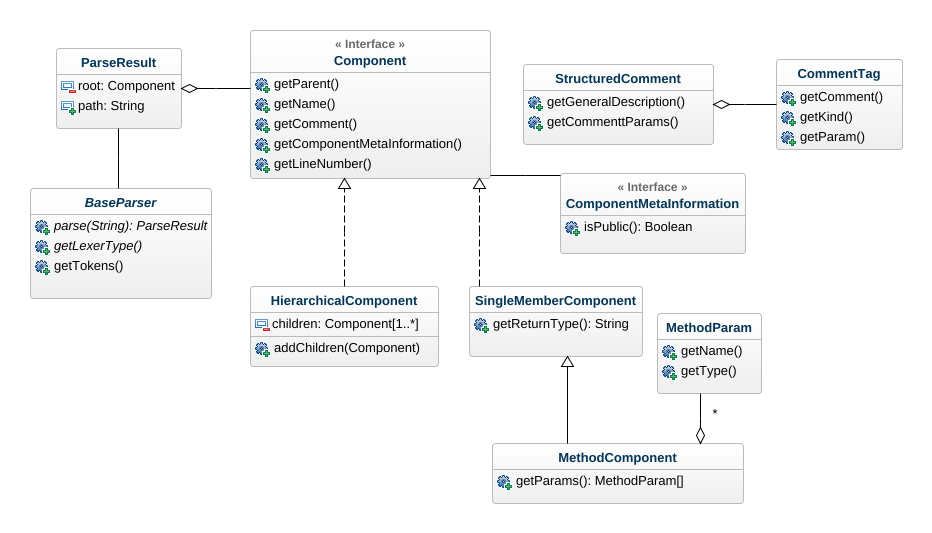
\includegraphics[height=9cm,keepaspectratio,angle=90]{figures/uml/parsing.png}
    \caption{UML-Diagramme aller Klassen, die relevant für das Parsen sind}
    \label{fig:uml_parsing}
\end{figure}
\chapter{UML-Diagramm: Metriken}\label{appendix_metrics_uml}
\begin{figure}[ht!]
\fontsize{5}{10}\selectfont
    \centering
    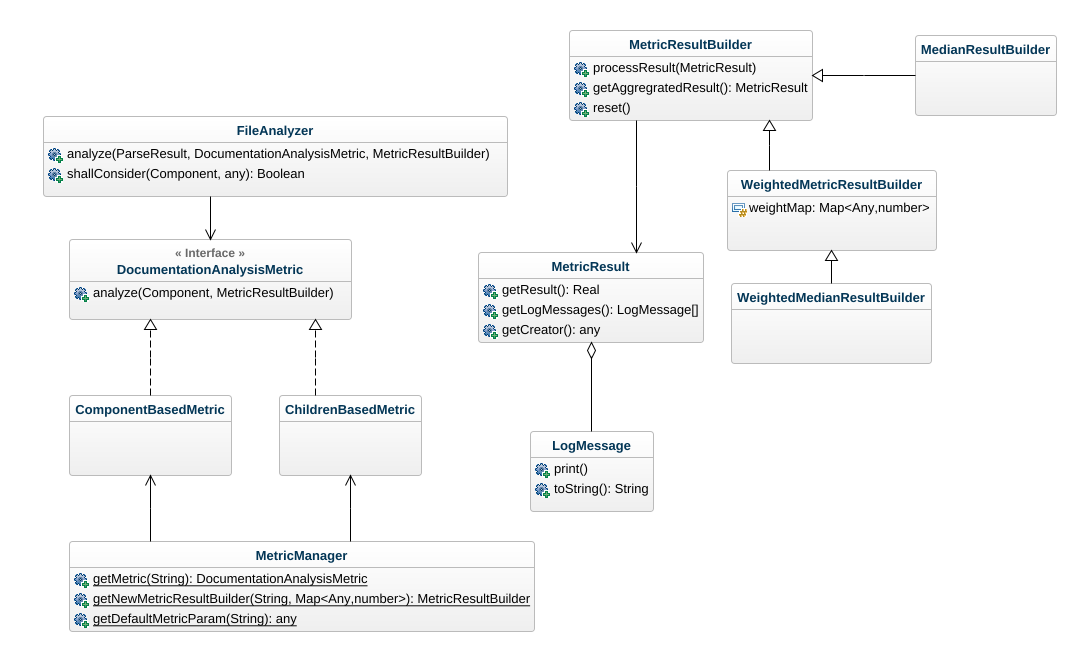
\includegraphics[height=10cm,keepaspectratio,angle=90]{figures/uml/metriken.png}
    \caption{UML-Diagramme aller Klassen, die relevant für die Metriken sind}
    \label{fig:uml_metrics}
\end{figure}
\chapter{Konfiguration des Tools}
\begin{description}
        \item[include]  Alle Dateien, die bei der Bewertung der Dokumentationsqualität berücksichtigt werden müssen
        \item[Exclude]  Teilmenge von include, enthält Dateien, die nicht weiter betrachtet werden müssen
        \item[metrics]  Alle Metriken, die das Tool verwenden soll. Dies ist ein Array von Objekten mit der Struktur \enquote{(name,weight, unique\_name, params)}, wobei \textit{weight} das Gewicht der jeweiligen Metrik ist (Bei Algorithmen ohne Relevanz des Gewichts wird es ignoriert), \textit{name} der Name der Metrik und \textit{params} ein Objekt mit den Parametern der Metrik
        \item[absolute\_threshold] Mindestwert der Bewertung, die erreicht werden muss, sonst wird die Dokumentationsqualität nicht akzeptiert
       
          \item[builder] Der Algorithmus/\textit{ResultBuilder}, der die einzelnen Ergebnisse verarbeitet.
        
        \item[parser]  Kann verwendet, um die zu parsende Programmiersprache zu wählen. Dazu muss \textit{ParserFactory} angepasst werden
        
        \item[path\_weights] Ein Array von Objekten der Struktur \enquote{(path,weight)}. Wird verwendet, um einzelne Pfade höher oder niedriger zu gewichtet
        
         \item[component\_weights] Ein Array von Objekten der Struktur \enquote{(name,weight)}. Wird verwendet, um einzelne Komponenten höher oder niedriger zu gewichtet
         
         \item[default\_path\_weight] Das Standardgewicht für eine Datei, wenn keine passende Gewichtung gefunden wurde
         
         \item[default\_component\_weight] Das Standardgewicht einer Komponente, wenn keine passende Gewichtung gefunden wurde
         
         \item[state\_manager] Kann verwendet werden, um festzulegen, wie das letzte Ergebnis der Dokumentationsqualität gespeichert werden soll. Weitere Möglichkeiten können durch Erweiterung der \textit{StateManagerFactory} hinzugefügt werden.
         
         \item[relative\_threshold] Der maximale  relative Abstand zur letzten Dokumentationsqualität bevor eine Fehlermeldung geworfen wird.
         \item[builder\_params] Parameter für die \textit{MetricResultBuilder}. Diese wird aktuell nur von dem Squale-Builder (Kapitel \ref{chapter:squale}) genutzt
        
        
        
    \label{enum:tool_javadoc_conf}
\end{description}
\chapter{Implementierte Metriken}\label{appendix_metrics}

\begin{description}

\item[Anteil dokumentierter Komponenten an allen Komponenten]
\begin{description}
\item[]
    \item [Metrikname]  simple\_comment
    \item [Klassenname] SimpleCommentPresentMetric
    \item[Beschreibung] Berechnet den Anteil der dokumentierten Komponenten an allen Komponenten, kann Getter und Setter ignorieren
    \item[Quellen] \cite[S. 5]{HowDocumentationEvolvesoverTime}
\end{description}

\item[Anteil öffentlicher dokumentierter Komponenten]
\begin{description}
\item[]
    \item [Metrikname]  public\_members\_only
    \item [Klassenname] SimplePublicMembersOnlyMetric
    \item[Beschreibung] Berechnet den Anteil der öffentlichen dokumentierten Komponenten an allen öffentlichen Komponenten, kann Getter und Setter ignorieren
     \item[Quellen] \cite[S. 253]{JavadocViolationsandTheirEvolutioninOpen-SourceSoftware}
\end{description}

\item[Bestrafung langer undokumentierter Methoden]
\begin{description}
\item[]
    \item [Metrikname]  large\_method\_commented
    \item [Klassenname] SimpleLargeMethodCommentedMetric
    \item[Beschreibung] Bestraft undokumentierte Methoden je nach ihrer Länge
    \item[Quellen] Eigene Idee
\end{description}

\item[Vollständigkeit der Dokumentation von Methoden]
\begin{description}
\item[]
    \item [Metrikname]  method\_fully\_documented
    \item [Klassenname] SimpleMethodDocumentationMetric
    \item[Beschreibung] Prüft, ob alle Methodenparameter und Rückgabewert dokumentiert sind
    \item[Quellen] \cite[S. 5]{HowDocumentationEvolvesoverTime}
\end{description}

\item[Anteil dokumentierter Methoden unter
Berücksichtigung der LOC]
\begin{description}
\item[]
    \item [Metrikname]  commented\_lines
    \item [Klassenname] CommentedLinesRatioMetric
    \item[Beschreibung]  Berechnet den Anteil der \ac{LOC} der dokumentierten Methoden an allen \ac{LOC} aller Methoden
    \item[Quellen] Eigene Idee
\end{description}

\item[Flesch-Score]
\begin{description}
\item[]
    \item [Metrikname]  flesch
    \item [Klassenname] FleschMetric
    \item[Beschreibung]   Berechnet den Flesch-Score des Kommentars und bewertet so, ob der Kommentar verständlich ist
    \item[Quellen] \cite[S. 72]{AutomaticQualityAssessmentofSourceCodeComments:TheJavadocMiner}
\end{description}

\item[Kohärenz zwischen Kommentar und
Komponentenname]
\begin{description}
\item[]
    \item [Metrikname]  comment\_name\_coherence
    \item [Klassenname] CommentNameCoherenceMetric
    \item[Beschreibung]  Prüft, ob der Kommentar und der Name der dokumentierten Komponente sehr ähnlich sind oder keine Ähnlichkeit haben, arbeitet nur mit Methoden
    \item[Quellen] \cite[S. 86ff ]{Qualityanalysisofsourcecodecomments}
\end{description}

\item[Verwendung bestimmter Wörter bestrafen]
\begin{description}
\item[]
    \item [Metrikname]  certain\_terms
    \item [Klassenname] CertainTermCountMetric
    \item[Beschreibung]  Bestraft das Vorkommen bestimmter Wörter (wie z.~B. Abkürzungen)
     \item[Quellen] Inspiriert von Verbot lateinischer Ausdrücke nach \cite{HowtoWriteDocCommentsfortheJavadocTool}
\end{description}

\item[Bewertung der Formatierung]
\begin{description}
\item[]
    \item [Metrikname]  formatting\_good
    \item [Klassenname] FormattingGoodMetric
    \item[Beschreibung] Überprüft, ob korrekte Tags verwendet wurde, HTML-Tags geschlossen wurden und bei langen Methoden überhaupt eine Formatierung verwendet wurden
     \item[Quellen] Inspiriert von Regel in Checkstyle \cite{checkstyle_doc_metrics}
\end{description}


\item[Rechtschreibfehler bestrafen] 

\begin{description}
\item[]
    \item [Metrikname]  spellling
    \item [Klassenname] SpellingMetric
    \item[Beschreibung]Sucht nach Rechtschreibfehlern und bestraft sie
    \item[Quellen] Eigene Idee
\end{description}

\item[Erwähnung von Randfällen bei Methodenparameter
und -rückgabewerte]
\begin{description}
\item[]
    \item [Metrikname]  edge\_case
    \item [Klassenname] EdgeCaseMetric
    \item[Beschreibung] Prüft, ob bei der Dokumentation von Parametern die Behandlung des Wertes \textit{null} erwähnt wird
       \item[Quellen] Inspiriert von Idee in  \cite{javadoc_coding_standards}. In \cite[S.~1ff.]{@tComment:TestingJavadocCommentstoDetectComment-CodeInconsistencies} wird ebenfalls auf einer ähnlichen Art und Weise die Erwähnung von Randfällen geprüft, dort aber auch, ob diese Angaben korrekt sind
\end{description}


\item[Gunning-Fog-Index]
\begin{description}
\item[]
    \item [Metrikname]  gunning\_fog
    \item [Klassenname] GunningFogMetric
    \item[Beschreibung] Berechnet den Gunning-Fog-Index des Kommentars und bewertet so, ob der Kommentar verständlich ist
     \item[Quellen] \cite[S. 71]{AutomaticQualityAssessmentofSourceCodeComments:TheJavadocMiner}
\end{description}
 \end{description}

\chapter{Bilder des Tools}\label{chapter:pictures_tool}
In diesem Kapitel sind zwei Bilder des \textit{DoxEvaluators} abgedruckt, welche die zwei möglichen Ausgaben des Programms zeigen (Dokumentationsqualität ausreichend und nicht ausreichend):
\begin{figure}[htbp!]
    \centering
    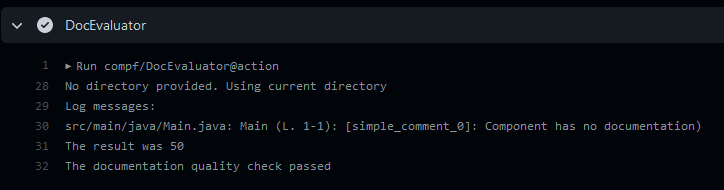
\includegraphics[width=\columnwidth]{figures/appendix/passed.png}
    \caption{Foto vom Tool: Dokumentationsqualität ausreichend}
    \label{fig:passed}
\end{figure}
\begin{figure}[htbp!]
    \centering
    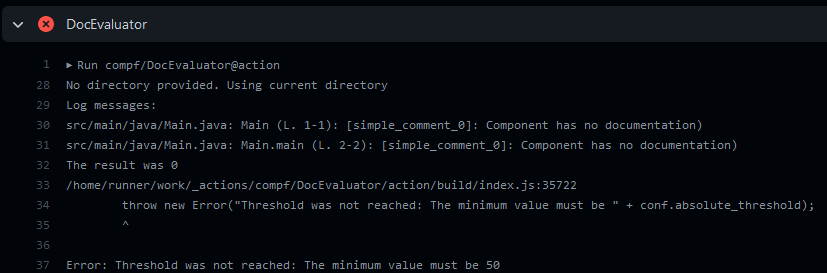
\includegraphics[width=\columnwidth]{figures/appendix/absolute_threshold.png}
    \caption{Foto vom Tool: Dokumentationsqualität zu schlecht}
    \label{fig:absolute}
\end{figure}

\end{appendices}
	



\chapter*{Erklärung zur selbstständigen Abfassung der Masterarbeit}

Ich versichere, dass ich die eingereichte Masterarbeit selbstständig und ohne unerlaubte Hilfe verfasst habe. Anderer als der von mir angegebenen Hilfsmittel und Schriften habe ich mich nicht bedient. Alle wörtlich oder sinngemäß den Schriften anderer Autoren entnommenen Stellen habe ich kenntlich gemacht. \\


\bigskip
\bigskip
\bigskip
\bigskip
\noindent
Osnabrück, 18. Oktober 2018 \\

\bigskip
\bigskip
\bigskip
\bigskip
\noindent
Vorname Nachname
\end{document}

